% $Id$
%\def\QM {{,\kern -0.9 pt ,}}
\setcounter{satz}{0}
\setcounter{definition}{0}

% ..........................................................................
% --------------------------------------------------------------------------
% ++++++++++++++++++++++++++++++++++++++++++++++++++++++++++++++++++++++++++
%              E l e m e n t a r e  Z a h l e n t h e o r i e
% /~~~~~~~~~~~~~~~~~~~~~~~~~~~~~~~~~~~~~~~~~~~~~~~~~~~~~~~~~~~~~~~~~~~~~~~~~

\newpage
\hypertarget{Chapter_ElementaryNT}{}

\section{Einf"uhrung in die elementare Zahlentheorie mit Beispielen}
\label{Chapter_ElementaryNT}
(Bernhard Esslinger, Juli 2001, Updates: Nov. 2001, Juni 2002, Mai 2003, Mai 2005) \\

Diese \glqq Einf"uhrung\grqq~ bietet einen Einstieg f"ur mathematisch Interessierte.
Erforderlich sind nicht mehr Vorkenntnisse als die, die im Grundkurs Mathematik am Gymnasium vermittelt werden.\par
Wir haben uns bewusst an \glqq Einsteigern\grqq~ und \glqq Interessenten\grqq~ orientiert, und nicht an den
Gepflogenheiten mathematischer Lehrb"ucher, die auch dann \glqq Einf"uhrung\grqq~ genannt werden,
wenn sie schon auf der 5. Seite nicht mehr auf Anhieb zu verstehen sind und sie eigentlich den Zweck haben, dass
man danach auch spezielle Monographien zu dem Thema lesen k"onnen soll.



% ++++++++++++++++++++++++++++++++++++++++++++++++++++++++++++++++++++++++++
\subsection{Mathematik und Kryptographie}
Ein gro"ser Teil der modernen, asymmetrischen Kryptographie beruht auf 
mathematischen Erkenntnissen -- auf den Eigenschaften (\glqq Gesetzen'')
ganzer Zahlen, die in der elementaren \index{Zahlentheorie!elementare}
Zahlentheorie untersucht werden. \glqq Elementar\grqq\ bedeutet hier, 
dass die zahlentheoretischen Fragestellungen im wesentlichen
in der Menge der nat"urlichen und der ganzen Zahlen durchgef"uhrt werden.

Weitere mathematische Disziplinen, die heute in der Kryptographie 
Verwendung finden, sind 
(vgl. \cite[S. 2]{Bauer1995}, \cite[Seite 3]{Bauer2000}) :
\begin{itemize}
    \item Gruppentheorie
    \item Kombinatorik
    \item Komplexit"atstheorie
    \item Ergodentheorie
    \item Informationstheorie.
\end{itemize}

Die Zahlentheorie oder Arithmetik (hier wird mehr der Aspekt des Rechnens
mit Zahlen betont) wurde von Carl Friedrich Gauss\footnote{%
  Carl Friedrich Gauss, deutscher Mathematiker und Astronom,
  30.4.1777$-$23.2.1855.
}
\index{Gauss, Carl Friedrich}
als besondere mathematische Disziplin begr"undet. Zu ihren elementaren
Gegenst"anden geh"oren: gr"o"ster gemeinsamer Teiler\footnote{%
Auf ggT\index{ggT}, englisch gcd (greatest common divisor), geht dieser
Artikel im \hyperlink{Appendix_A}{Anhang A zu diesem Kapitel} ein.
} (ggT), Kongruenzen (Restklassen), Faktorisierung, Satz von Euler-Fermat und
primitive Wurzeln. Kernbegriff sind jedoch die Primzahlen und ihre
multiplikative Verkn"upfung.

Lange Zeit galt gerade die Zahlentheorie als Forschung pur, als
Paradebeispiel f"ur die Forschung im Elfenbeinturm. Sie erforschte die
\glqq geheimnisvollen Gesetze im Reich der Zahlen'' und gab Anlass zu
philosophischen Er"orterungen, ob sie beschreibt, was "uberall in der Natur
schon da ist, oder ob sie ihre Elemente (Zahlen, Operatoren, Eigenschaften)
nicht k"unstlich konstruiert.

Inzwischen wei"s man, dass sich zahlentheoretische Muster "uberall in der Natur
finden. Zum Beispiel verhalten sich die Anzahl der links- und der
rechtsdrehenden Spiralen einer Sonnenblume zueinander wie zwei
aufeinanderfolgende\index{Fibonacci} Fibonacci-Zahlen\footnote{%
Die Folge der Fibonacci-Zahlen $(a_i)_{i \in \mathbb{N}}$ ist definiert durch die \glqq rekursive'' 
Vorschrift $a_1 := a_2 := 1$ und f"ur alle Zahlen  $n=1,2,3,\cdots$ definiert man 
$a_{n+2} := a_{n+1}+a_n$.  Zu dieser historischen Folge gibt es viele interessante 
Anwendungen in der Natur (siehe z.B. \cite[S. 290 ff]{Graham1994}\index{Graham 1994} oder die Web-Seite 
von \hyperlink{knott}{Ron Knott:} \index{Knott, Ron} hier dreht sich alles um Fibonacci-Zahlen). 
Die Fibonacci-Folge\index{Fibonacci} ist gut verstanden und wird heute als wichtiges Werkzeug in der 
Mathematik benutzt.
}, also z.B.  wie  $21 : 34$.

Au"serdem wurde sp"atestens mit den zahlentheoretischen Anwendungen der
modernen Kryptographie klar, dass eine jahrhundertelang als theoretisch
geltende Disziplin praktische Anwendung findet, nach deren Experten heute
eine hohe Nachfrage auf dem Arbeitsmarkt besteht.

Anwendungen der (Computer-)Sicherheit bedienen sich heute der Kryptographie,
weil Kryptographie als mathematische Disziplin einfach besser und
beweisbarer ist als alle im Laufe der Jahrhunderte erfundenen \glqq kreativen''
Verfahren der Substitution und besser als alle ausgefeilten physischen
Techniken wie beispielsweise beim Banknotendruck \cite[S. 4]{Beutelspacher1996}.

In diesem Artikel werden in einer leicht verst"andlichen Art die
grundlegenden Erkenntnisse der elementaren Zahlentheorie anhand vieler
Beispiele vorgestellt -- auf Beweise wird (fast) vollst"andig verzichtet
(diese finden sich in den mathematischen Lehrb"uchern).

Ziel ist nicht die umfassende Darstellung der zahlentheoretischen Erkenntnisse,
sondern das Aufzeigen der wesentlichen Vorgehensweisen. Der Umfang des Stoffes
orientiert sich daran, das RSA-Verfahren\index{RSA} verstehen und anwenden
zu k"onnen.

Dazu wird sowohl an Beispielen als auch in der Theorie erkl"art, wie man in
endlichen Mengen rechnet und wie dies in der Kryptographie Anwendung findet.
Insbesondere wird auf die klassischen Public Key-Verfahren Diffie-Hellman
\index{Diffie-Hellman} (DH) und RSA\index{RSA} eingegangen.

Au"serdem war es mir wichtig, fundierte Aussagen zur Sicherheit des RSA-Verfahrens zu machen.

\vskip +40 pt

\begin{center}
\fbox{\parbox{15cm}{{\em Carl Friedrich Gauss:\index{Gauss, Carl Friedrich}}\\
Die Mathematik ist die K"onigin der Wissenschaften, die Zahlentheorie aber
ist die K"onigin der Mathematik.}}
\end{center}


% ++++++++++++++++++++++++++++++++++++++++++++++++++++++++++++++++++++++++++
\subsection{Einf"uhrung in die Zahlentheorie}
\index{Zahlentheorie!Einf""uhrung} 

Die Zahlentheorie entstand aus Interesse an den positiven ganzen Zahlen $1,
2, 3, 4, \cdots ,$ die auch als die Menge der \index{Zahlen!nat""urliche}
{\em nat"urlichen Zahlen} $\mathbb{N}$ bezeichnet
werden. Sie sind die ersten mathematischen Konstrukte der menschlichen
Zivilisation. Nach Kronecker\footnote{%
Leopold Kronecker, deutscher Mathematiker, 7.12.1823$-$29.12.1891.
}
\index{Kronecker, Leopold} hat sie der liebe Gott geschaffen, 
nach Dedekind\footnote{Julius Wilhelm Richard Dedekind,
deutscher Mathematiker, 06.10.1831$-$12.02.1916.
}
\index{Dedekind, Julius} der menschliche Geist.
Das ist je nach Weltanschauung ein unl"osbarer Widerspruch oder
ein und dasselbe.

Im Altertum gab es keinen Unterschied zwischen Zahlentheorie und
Numerologie, die einzelnen Zahlen mystische Bedeutung zuma"s. So wie sich
w"ahrend der Renaissance (ab dem 14. Jahrhundert) die Astronomie allm"ahlich
von der Astrologie und die Chemie von der Alchemie l"oste, so lie"s auch die
Zahlentheorie die Numerologie hinter sich.

Die Zahlentheorie faszinierte schon immer Amateure wie auch professionelle
Mathematiker. Im Unterschied zu anderen Teilgebieten der Mathematik k"onnen
viele der Probleme und S"atze auch von Laien verstanden werden, andererseits
widersetzten sich die L"osungen zu den Problemen und die Beweise zu den S"atzen
oft sehr lange den Mathematikern. Es ist also leicht, gute Fragen zu stellen,
aber es ist ganz etwas anderes, die Antwort zu finden. Ein Beispiel daf"ur ist
der sogenannte letzte (oder gro"se) Satz von Fermat\footnote{Thema der
	Schul-Mathematik ist der Satz von Pythagoras\index{Pythagoras!Satz von},
	wo gelehrt wird, dass in einem
	rechtwinkligen Dreieck gilt: $a^2 + b^2 = c^2$, wobei $a, b$ die
	Schenkell"angen sind und c die L"ange der Hypothenuse ist. Fermats ber"uhmte
	Behauptung war, dass f"ur ganzzahlige Exponenten $n > 2$ immer die
	Ungleichheit $a^n + b^n \not= c^n$ gilt. Leider fand \index{Fermat!letzter
	Satz} Fermat auf dem Brief, wo er die Behauptung aufstellte, nicht gen"ugend
	Platz, um den Satz zu beweisen. Der Satz konnte erst "uber 300 Jahre sp"ater
	bewiesen werden \cite[S.  433-551]{Wiles1994}. \index{Wiles, Andrew}
}.

Bis zur Mitte des 20. Jahrhunderts wurde die Zahlentheorie als das reinste
Teilgebiet der Mathematik angesehen -- ohne Verwendung in der wirklichen Welt.
Mit dem Aufkommen der Computer und der digitalen Kommunikation "anderte sich
das: die Zahlentheorie konnte einige unerwartete Antworten f"ur reale
Aufgabenstellungen liefern. Gleichzeitig halfen die Fortschritte in der EDV,
dass die Zahlentheoretiker gro"se Fortschritte machten im Faktorisieren gro"ser
Zahlen, in der Bestimmung neuer Primzahlen, im Testen von (alten)
Vermutungen und beim L"osen bisher unl"osbarer numerischer Probleme.

Die moderne Zahlentheorie \index{Zahlentheorie!moderne} besteht aus Teilgebieten wie
\begin{itemize}
    \item Elementare Zahlentheorie
    \item Algebraische Zahlentheorie
    \item Analytische Zahlentheorie
    \item Geometrische Zahlentheorie
    \item Kombinatorische Zahlentheorie
    \item Numerische Zahlentheorie und
    \item Wahrscheinlichkeitstheorie.
\end{itemize}

Die verschiedenen Teilgebiete besch"aftigen sich alle mit Fragestellungen zu
den ganzen Zahlen (positive und negative ganze Zahlen und die Null), gehen
diese jedoch mit verschiedenen Methoden an.

Dieser Artikel besch"aftigt sich nur mit dem Teilgebiet der elementaren
Zahlentheorie.
\newpage


% --------------------------------------------------------------------------
\subsubsection{Konvention}
Wird nichts anderes gesagt, gilt: 
\begin{itemize}
\item Die Buchstaben $a, b, c, d, e, k, n, m, p, q$ stehen f"ur ganze Zahlen.
\item Die Buchstaben $i$ ~\mbox{und} ~$j$ stehen f"ur nat"urliche Zahlen. 
\item Der Buchstabe $p$ steht stets f"ur eine Primzahl.
\item Die Mengen $\mathbb{N} = \{ 1, 2, 3, \cdots \}$ und $\mathbb{Z} =\{ \cdots, -3, -2, -1, 0, 1, 2, 3, \cdots \}$ 
sind die {\em nat"urlichen} und die {\em ganzen} Zahlen.
\end{itemize}



%\vskip +40 pt
\newpage

\begin{center}
\fbox{\parbox{15cm}{{\em Joanne K. Rowling\index{Rowling, Joanne}\footnotemark:}\newline Das ist nicht Zauberei, das ist Logik, ein R"atsel.
Viele von den gr"o"sten Zauberern haben keine Unze Logik im Kopf.}}
\end{center}
\addtocounter{footnote}{0}\footnotetext{Joanne K. Rowling,~\glqq Harry Potter und der Stein der Weisen'', Carlsen, (c)
1997, Kapitel ~\glqq Durch die Fallt"ur'', S. 310, Hermine.}


% ++++++++++++++++++++++++++++++++++++++++++++++++++++++++++++++++++++++++++
\subsection{Primzahlen und der erste Hauptsatz der elementaren Zahlentheorie}
\index{Zahlentheorie!elementare} Viele der Probleme in der elementaren Zahlentheorie besch"aftigen sich mit
Primzahlen.

Jede ganze Zahl hat Teiler oder Faktoren. Die Zahl 1 hat nur einen, n"amlich
sich selbst. Die Zahl 12 hat die sechs Teiler 1, 2, 3, 4, 6 und 12\footnote{%
Aufgrund der gro"sen Teilerzahl von 12 findet sich diese Zahl -- und Vielfache dieser Zahl -- oft im allt"aglichen wieder:
Die 12 Stunden-Skala der Uhr, die 60 Minuten einer Stunde, die 360 Grad-Skala der Winkelmessung, usw. Teilt man 
diese Skalen in Bruchteile auf, so ergeben sich in vielen F"allen die Br"uche als ganze Zahlen. Mit diesen kann 
man im Kopf einfacher rechnen als mit gebrochenen Zahlen.
}. Viele Zahlen sind nur teilbar durch sich selbst und durch 1. Bez"uglich der
Multiplikation sind dies die \glqq Atome'' im Bereich der Zahlen.

\index{Primzahl}
\begin{definition}\label{def-zth-prime} 
{\bf Primzahlen} sind nat"urliche Zahlen gr"o"ser als $1$, die nur durch $1$ und sich
selbst teilbar sind.
\end{definition}

Per Definition ist $1$ keine Primzahl.

Schreibt man die Primzahlen in aufsteigender Folge (Primzahlenfolge), so
ergibt sich
$$2,~ 3,~ 5,~ 7,~ 11, ~13,~ 17,~ 19, ~23, ~29, ~31, ~37,~ 41,~ 43,~ 47,~ 53, ~59, ~61, ~67, ~71,
~73, ~79, ~83, ~89, ~97, \cdots.$$

Unter den ersten $100$ Zahlen gibt es genau $25$ Primzahlen. Danach nimmt ihr
prozentualer Anteil ab, wird aber nie Null.

Primzahlen treten als ganze Zahlen nicht selten auf. Allein im letzten
Jahrzehnt waren drei Jahre prim: $1993, 1997$ und $1999$. W"aren sie selten,
k"onnte die Kryptographie auch nicht so mit ihnen arbeiten, wie sie es tut.

Primzahlen k"onnen nur auf eine einzige (\glqq triviale'') Weise zerlegt werden:
\begin{eqnarray*}
5 & = & 1 * 5 \nonumber \\
17 & =  & 1 * 17 \nonumber \\
1.013 &  = & 1 * 1.013 \nonumber \\
1.296.409 & = & 1 * 1.296.409. \nonumber
\end{eqnarray*}

\index{Zahlen!zusammengesetzte}
\begin{definition}\label{def-zth-composite} 
Nat"urliche Zahlen gr"o"ser $1$, die keine Primzahlen sind, hei"sen
{\bf zusammengesetzte Zahlen}: diese haben mindestens zwei von $1$ verschiedene
Faktoren.
\end{definition}


Beispiele f"ur die Primfaktorzerlegung\index{Primfaktor!Zerlegung} solcher
Zahlen:
\begin{eqnarray*}
4 & = & 2*2  \nonumber \\
6 & = & 2*3  \nonumber \\
91 & = & 7*13  \nonumber \\
161 & = & 7*23  \nonumber \\
767 & = & 13*59  \nonumber \\
1.029 & = & 3 * 7^3  \nonumber \\
5.324 & = & 22 * 11^3.  \nonumber 
\end{eqnarray*}

\begin{satz}\label{thm-zth-cnum}
Jede zusammengesetzte Zahl $a$ besitzt einen kleinsten Teiler gr"o"ser
als $1$. Dieser Teiler ist eine Primzahl $p$ und kleiner oder gleich der Quadratwurzel
aus $a$.
\end{satz}

Aus den Primzahlen lassen sich alle ganzen Zahlen gr"o"ser als $1$
zusammensetzen -- und das sogar in einer {\em eindeutigen} Weise.

Dies besagt \index{Zahlentheorie!Hauptsatz} der 1. {\em Hauptsatz der Zahlentheorie} (= Hauptsatz der elementaren
Zahlentheorie = fundamental theorem of arithmetic = fundamental building
block of all positive integers). Er wurde das erste Mal pr"azise von Carl
Friedrich Gauss in seinen Disquisitiones Arithmeticae (1801) formuliert. 
\index{Zahlentheorie!Hauptsatz}  \index{Gauss, Carl Friedrich}

\begin{satz}{\bf Gauss 1801}\label{thm-zth-mthm}
Jede nat"urliche Zahl $a$ gr"o"ser als $1$ l"asst sich als Produkt von
Primzahlen schreiben. Sind zwei solche Zerlegungen $a = p_1*p_2*\cdots*p_n = q_1*q_2*\cdots*q_m$ gegeben, dann
gilt nach eventuellem Umsortieren $n = m$ und f"ur alle $i$: $p_i = q_i$.
\end{satz}

In anderen Worten: Jede nat"urliche Zahl au"ser der $1$ l"asst sich auf genau eine
Weise als Produkt von Primzahlen schreiben, wenn man von der Reihenfolge der
Faktoren absieht. Die Faktoren sind also eindeutig (die \glqq Expansion in
Faktoren'' ist eindeutig)!

Zum Beispiel ist $60 = 2*2*3*5 = 2^2*3*5$. Und das ist --- bis auf eine
ver"anderte Reihenfolge der Faktoren --- die einzige M"oglichkeit, die Zahl $60$
in Primfaktoren\index{Primfaktor} zu zerlegen.

Wenn man nicht nur Primzahlen als Faktoren zul"asst, gibt es mehrere
M"oglichkeiten der Zerlegung in Faktoren und die {\em Eindeutigkeit} (uniqueness)
geht verloren:
$$60 = 1*60 = 2*30 = 4*15 = 5*12 = 6*10 = 2*3*10 = 2*5*6 = 3*4*5 = \cdots$$
Der 1. Hauptsatz ist nur scheinbar selbstverst"andlich. Man kann viele andere
Zahlenmengen\footnote{%
Diese Mengen werden speziell aus der Menge der nat"urlichen Zahlen gebildet.
Ein Beispiel findet sich in diesem \hyperlink{uniqueness}{Skript}
auf Seite~\pageref{thm-pz-euklid} %eigentlich \pageref{remFundTheoOfArithm},
%aber hyperref ist buggy
am Ende von Kapitel~\ref{primesinmath}.
}
konstruieren, bei denen eine multiplikative Zerlegung in die Primfaktoren
dieser Mengen {\em nicht} eindeutig ist.

F"ur eine mathematische Aussage ist es deshalb nicht nur wichtig, f"ur welche
Operation sie definiert wird, sondern auch auf welcher Grundmenge diese
Operation definiert wird.

Weitere Details zu den Primzahlen (z.B. wie der \glqq Kleine Satz von 
Fermat'' zum Testen von sehr gro"sen Zahlen auf ihre Primzahleigenschaft
benutzt werden kann) finden sich in diesem Skript in dem Artikel "uber 
\hyperlink{Kapitel_2}{Primzahlen, Kapitel \ref{Label_Kapitel_2}}.


% ++++++++++++++++++++++++++++++++++++++++++++++++++++++++++++++++++++++++++
\subsection{Teilbarkeit, Modulus und Restklassen}
\index{Modulus} \index{Teilbarkeit} Werden ganze Zahlen addiert, subtrahiert oder multipliziert, ist das
Ergebnis stets wieder eine ganze Zahl.

Die Division zweier ganzer Zahlen ergibt nicht immer eine ganze Zahl. Wenn
man z.B. $158$ durch $10$ teilt, ist das Ergebnis die Dezimalzahl $15,8$. Dies ist
keine ganze Zahl!

Teilt man $158$ dagegen durch $2$, ist das Ergebnis $79$ eine ganze Zahl.
In der Zahlentheorie sagt man, $158$ ist {\em teilbar} durch $2$, aber nicht durch $10$.
Allgemein sagt man:

\begin{definition}\label{def-zth-divisibility} \index{Teilbarkeit} \index{teilbar}
Eine ganze Zahl $n$ ist {\bf teilbar} durch eine ganze Zahl $d$, wenn der Quotient $n/d$
eine ganze Zahl $c$ ist, so dass $n = c * d$.
\end{definition}

Die Zahl $n$ wird {\em Vielfaches} von $d$ genannt; $d$ wird {\em Teiler, Divisor} \index{Teiler} \index{Divisor} oder \index{Faktor} {\em Faktor} von $n$
genannt.

Mathematisch schreibt man das: $d | n$ (gelesen: \glqq  $d$ teilt $n$'').
Die Schreibweise $d \!\!\not| n$ bedeutet, dass $d$ die Zahl $n$ nicht teilt.

Also gilt in unserem obigen Beispiel: $10\!\!\not| 158$, aber $2 | 158$.


% --------------------------------------------------------------------------
\subsubsection{Die Modulo-Operation -- Rechnen mit Kongruenzen} \index{Kongruenz}

Bei Teilbarkeitsuntersuchungen kommt es nur auf die Reste der Division an:
Teilt man eine Zahl $n$ durch $m$, so benutzt man oft die folgende Schreibweise:
$$\frac{n}{m} = c + \frac{r}{m} ,$$
wobei $c$ eine ganze Zahl ist und $r$ eine Zahl mit den Werten $0,1,\cdots, m-1$.
Diese Schreibweise hei"st Division mit Rest. Dabei hei"st $c$ der ganzzahlige 
\glqq Quotient'' und $r$ der \glqq Rest'' der Division.

{\bf Beispiel:} \\
$$\frac{19}{7} = 2 + \frac{5}{7} \quad (m=7, c = 2, r = 5)$$

Was haben die Zahlen $5, 12, 19, 26, \cdots$ bei der Division durch $7$ gemeinsam?
Es ergibt sich immer der Rest $r = 5$.
Bei der Division durch $7$ sind nur die folgenden Reste m"oglich:
$$r = 0, 1, 2, \cdots, 6.$$

Wir fassen bei der Division durch $7$ die Zahlen, die den gleichen Rest $r$
ergeben, in die \glqq Restklasse $r$ modulo $7$'' zusammen. Zwei Zahlen $a$ und $b$, die
zur gleichen Restklasse modulo $7$ geh"oren, bezeichnen wir als \glqq kongruent
modulo 7''. Oder ganz allgemein:

\begin{definition}\label{def-zth-remainder} \index{Restklasse}
Als {\bf Restklasse $r$ modulo $m$} bezeichnet man alle ganzen Zahlen $a$, die bei der Division 
durch $m$ denselben Rest $r$ haben.
\end{definition}
\newpage
{\bf Beispiele:}
\begin{itemize}
\item[] Restklasse $0$ modulo $4 = \{ x | x = 4*n; \; n \in \mathbb{N} \} = \{ \dots, -16, -12, -8, -4, 0, 4, 8, 12, 16, \dots \}$
\item[] Restklasse $3$ modulo $4 = \{ x | x = 4*n + 3;\; n \in \mathbb{N} \} = \{ \dots, -13, -9, -5, -1, 3, 7, 11, 15, \dots \}$
\end{itemize}
Da modulo $m$ nur die Reste $0, 1, 2, \cdots, m-1$ m"oglich sind, rechnet die modulare Arithmetik in endlichen Mengen. 
Zu jedem Modul $m$ gibt es genau $m$ Restklassen.

\begin{definition}\label{def-zth-congruence} \index{Kongruenz}
Zwei Zahlen $a, b \in \mathbb{N}$  hei"sen \index{restgleich} \index{kongruent}
{\bf restgleich oder kongruent bez"uglich $m \in \mathbb{N}$}  genau dann, 
wenn beim Teilen durch $m$ der gleiche Rest bleibt.
\end{definition}

Man schreibt: $a \equiv b {\rm ~(mod~} m)$. Und sagt:  {\em $a$ ist kongruent $b$ modulo $m$}. Das bedeutet, 
dass $a$ und $b$ zur gleichen Restklasse geh"oren. Der Modul ist also der Teiler. Diese Schreibweise wurde von 
Gauss eingef"uhrt. Gew"ohnlich ist der Teiler positiv, aber $a$ und $b$ k"onnen auch beliebige ganze Zahlen sein.

{\bf Beispiele:}
\begin{itemize}
   \item[] $19 \equiv 12 {\rm ~(mod~} 7)$,         
           denn die Reste sind gleich:  $19 / 7 = 2$ Rest $5$  und  $12 / 7 = 1$ Rest $5$.
   \item[] $23103 \equiv 0 {\rm ~(mod~} 453)$, denn $23103 / 453 = 51$ Rest $0$  und  $0 / 453 = 0$ Rest $0$.
\end{itemize}

\begin{satz}\label{thm-zth-div}
$a \equiv b$ (mod $m$) gilt genau dann,  wenn die Differenz $(a - b)$ durch $m$ teilbar ist, also wenn 
ein $q\in \mathbf{Z}$ existiert mit $ (a-b)=q*m.$
\end{satz}
Diese beiden Aussagen sind also "aquivalent.

Daraus ergibt sich: Wenn $m$ die Differenz teilt, gibt es eine ganze Zahl $q$, so dass gilt: $a = b + q*m$.
Alternativ zur Kongruenzschreibweise kann man auch die Teilbarkeitsschreibweise verwenden: $m | (a - b)$.

{\bf Beispiel "aquivalenter Aussagen:} \\
$35 \equiv 11$ (mod $3) \Longleftrightarrow  35 - 11 \equiv 0$ (mod $3)$, 
wobei $35 - 11 = 24$ sich ohne Rest durch $3$ teilen l"asst, w"ahrend $35:3$ und $11:3$ beide den Rest $2$ ergeben.

{\bf Bemerkung:}\\
F"ur die Summe $(a + b)$ gilt die obige "Aquivalenz nicht!

{\bf Beispiel: }\\
$11 \equiv 2$ (mod $3$), also ist $11 - 2 \equiv 9 \equiv 0$ (mod $3$); aber $11 + 2 = 13$ ist nicht durch $3$ teilbar.
Die Aussage von Satz \ref{thm-zth-div} gilt f"ur Summen nicht einmal in eine
Richtung. Richtig ist sie bei Summen nur f"ur den Rest $0$ und nur in der
folgenden Richtung: Teilt ein Teiler beide Summanden ohne Rest, teilt er
auch die Summe ohne Rest.

Anwenden kann man die obige "Aquivalenz von Satz \ref{thm-zth-div}, wenn man schnell und
geschickt f"ur gro"se Zahlen entscheiden will, ob sie durch eine bestimmte
Zahl teilbar sind.

\newpage
{\bf Beispiel:} \\
Ist $69.993$ durch $7$ teilbar? \\
Da die Zahl in eine Differenz zerlegt werden kann, wo einfach zu ersehen
ist, dass jeder Operand durch $7$ teilbar ist, ist auch die Differenz durch $7$
teilbar: $69.993 = 70.000 - 7$.

Diese "Uberlegungen und Definitionen m"ogen recht theoretisch erscheinen, sind
uns im Alltag aber so vertraut, dass wir die formale Vorgehensweise gar nicht
mehr wahrnehmen: Bei der Uhr werden die $24$ h eines Tages durch die Zahlen $1$,
$2, \cdots, 12$ repr"asentiert. Die Stunden nach $12:00$ mittags erh"alt man als
Reste einer Division durch 12. Wir wissen sofort, dass $2$ Uhr nachmittags
dasselbe wie $14:00$ ist.

Diese \glqq modulare'', also auf die Divisionsreste bezogene Arithmetik ist die
Basis der asymmetrischen Verschl"usselungsverfahren.
Kryptographische Berechnungen spielen sich also nicht wie das Schulrechnen
unter den reellen Zahlen ab, sondern unter Zeichenketten begrenzter L"ange,
das hei"st unter positiven ganzen Zahlen, die einen gewissen Wert nicht
"uberschreiten d"urfen.
Aus diesem und anderen Gr"unden w"ahlt man sich eine gro"se Zahl $m$ und \glqq rechnet
modulo $m$'', das hei"st, man ignoriert ganzzahlige Vielfache von $m$ und rechnet
statt mit einer Zahl nur mit dem Rest bei Division dieser Zahl durch $m$.
Dadurch bleiben alle Ergebnisse im Bereich von $0$ bis $m-1$.


% ++++++++++++++++++++++++++++++++++++++++++++++++++++++++++++++++++++++++++
\subsection{Rechnen in endlichen Mengen}

% --------------------------------------------------------------------------
\subsubsection{Gesetze beim modularen Rechnen}

Aus S"atzen der Algebra folgt, dass wesentliche Teile der "ublichen
Rechenregeln beim "Ubergang zum modularen Rechnen "uber der Grundmenge $\mathbb{Z}$
erhalten bleiben: Die Addition ist nach wie vor kommutativ. Gleiches gilt f"ur die
Multiplikation modulo $m$. Das Ergebnis einer Division\footnote{%
\label{ftn-res-divmodn}Die Division modulo $m$\index{Division modulo $n$} ist nur f"ur Zahlen, die teilerfremd zu $m$ sind, definiert. 
Vergleiche Fu"ssnote \ref{ftn-mod6} in Kapitel \ref{addmult}.
} ist kein Bruch, sondern eine ganze Zahl zwischen $0$ und $m-1$.

Es gelten die bekannten Gesetze:
\begin{itemize}
\item[\bf 1.] {\bf Assoziativgesetz:}\index{Assoziativgesetz} \\ 
    $((a+b) + c) {\rm ~(mod~ } m) \equiv  (a + (b+c)) {\rm ~(mod~ } m).$ \\
    $((a*b) * c) {\rm ~(mod~ } m) \equiv  (a * (b*c)) {\rm ~(mod~ } m).$
\item[\bf 2.] {\bf Kommutativgesetz:} \index{Kommutativgesetz}\\
    $(a+b) {\rm ~(mod~ } m) \equiv  (b+a) {\rm ~(mod~ } m).$ \\
     $(a*b) {\rm ~(mod~ } m) \equiv  (b*a) {\rm ~(mod~ } m).$
\end{itemize}
Assoziativgesetz und Kommutativgesetz gelten sowohl f"ur die Addition als auch f"ur die Multiplikation.
\begin{itemize}
\item[\bf 3.] {\bf Distributivgesetz:} \index{Distributivgesetz}\\
    $ (a * (b+c)) {\rm ~(mod~ } m) \equiv  (a*b + a*c) {\rm ~(mod~ } m).$ 
\item[\bf 4.] {\bf Reduzierbarkeit:} \index{Reduzierbarkeit} \\
    $(a+b) {\rm ~(mod~} m) \equiv  (a {\rm ~(mod~ } m) + b {\rm ~(mod~ } m)) {\rm ~(mod~} m).$ \\  
    $(a*b) {\rm ~(mod~} m) \equiv  (a {\rm ~(mod~ } m) * b {\rm ~(mod~ } m)) {\rm ~(mod~} m).$
\end{itemize}
Es ist gleichg"ultig, in welcher Reihenfolge die Modulo-Operation durchgef"uhrt wird.
\begin{itemize}
\item[\bf 5.] {\bf Existenz einer Identit"at (neutrales Element):} \index{Identit""at}\\
    $(a + 0) {\rm ~(mod~ } m) \equiv  (0 + a) {\rm ~(mod~ } m) \equiv  a {\rm ~(mod~ } m).$  \\
    $(a * 1) {\rm ~(mod~ } m) \equiv  (1 * a) {\rm ~(mod~ } m) \equiv  a {\rm ~(mod~ } m).$
\item[\bf 6.] {\bf Existenz des inversen Elements:} \\
    F"ur jedes ganzzahlige $a$ und $m$ gibt es eine ganze Zahl $-a$, so dass gilt: \\
    $(a + (-a)) {\rm ~(mod~}m) \equiv  0 {\rm ~(mod~ } m)$ \quad (additive Inverse). \index{Inverse!additive}\\
    F"ur jedes $a$ ($a \not\equiv 0 {\rm ~(mod~ } p$) ) und $p$ prim gibt es eine ganze Zahl $a^{-1}$, so dass gilt: \\
    $(a * a^{-1}) {\rm ~(mod~ } p) \equiv 1 {\rm ~(mod~}p)$ \quad (multiplikative Inverse). \index{Inverse!multiplikative}
\item[\bf 7.] \index{Abgeschlossenheit} {\bf Abgeschlossenheit:}\footnote{%
\label{ftn-closed}Diese Eigenschaft wird innerhalb einer Menge immer bez"uglich einer Operation definiert. 
Siehe \hyperlink{Appendix_B}{Anhang B zu diesem Kapitel}.
} \\
$a, b \in G  \Longrightarrow  ( a + b ) \in G.$ \\
$a, b \in G  \Longrightarrow  ( a * b ) \in G.$
\item[\bf 8.] \index{Transitivit""at} {\bf Transitivit"at:}\\
$ [ a \equiv b {\rm ~mod~ } m, ~b \equiv c {\rm ~mod~ } m] \Longrightarrow [ a \equiv c {\rm ~mod~ } m].
$
\end{itemize}


% --------------------------------------------------------------------------
\subsubsection{Muster und Strukturen} \index{Struktur}
\hypertarget{Chapter_ElementaryNT_5_2}{}
\label{Label_Chapter_ElementaryNT_5_2}

Generell untersuchen die Mathematiker \glqq Strukturen\grqq. Sie fragen sich
z.B. bei $ a * x \equiv b {\rm ~mod~ } m, $ welche Werte $x$ f"ur gegebene 
Werte $a,b,m$ annehmen kann.

Insbesondere wird dies untersucht f"ur den Fall, dass das Ergebnis $b$ der 
Operation das neutrale Element ist. Dann ist $x$ die Inverse von $a$ 
bez"uglich dieser Operation.




\newpage
\begin{center}
\fbox{\parbox{15cm}{
    \emph{Seneca\index{Seneca}\footnotemark:}\\
    Lang ist der Weg durch Lehren, kurz und wirksam durch Beispiele.
}}
\end{center}
\addtocounter{footnote}{0}
\footnotetext{Lucius Annaeus Seneca, philosophischer Schriftsteller und
              Dichter, 4~v.~Chr. $-$ 65~n.~Chr.}

% ++++++++++++++++++++++++++++++++++++++++++++++++++++++++++++++++++++++++++
% \pagebreak
\subsection{Beispiele f"ur modulares Rechnen}

Wir haben bisher gesehen:

F"ur zwei nat"urliche Zahlen $a$ und $m$ bezeichnet  $a$ mod $m$  den Rest, den man erh"alt, 
wenn man $a$ durch $m$ teilt. Daher ist $a {\rm ~(mod~ } m$) stets eine Zahl zwischen $0$ und $m-1$.

Zum Beispiel gilt: $1 \equiv  6  \equiv  41 {\rm ~(mod~ } 5)$, denn der Rest ist jeweils $1$.

Ein anderes Beispiel ist: $2000  \equiv  0 {\rm ~(mod~ } 4)$, denn $4$ geht in $2000$ ohne Rest auf.

In der modularen Arithmetik gibt es nur eine eingeschr"ankte Menge
nicht-negativer Zahlen. Deren Anzahl wird durch einen Modul $m$ vorgegeben.
Ist der Modul $m = 5$, werden nur die 5 Zahlen der Menge $\{ 0, 1, 2, 3, 4\}$ benutzt.

Ein Rechenergebnis gr"o"ser als $4$ wird dann \glqq modulo'' $5$ umgeformt, d.h. es ist
der Rest, der sich bei der Division des Ergebnisses durch $5$ ergibt. So ist
etwa $2*4 \equiv 8 \equiv 3 {\rm ~(mod~ } 5)$, da $3$ der Rest ist, wenn man $8$ durch $5$ teilt.


% --------------------------------------------------------------------------
\subsubsection{Addition und Multiplikation} \index{Addition} \index{Multiplikation}\label{addmult}

Im folgenden werden 
\begin{itemize}
\item die Additionstabelle\footnote{%
Bemerkung zur Subtraktion modulo 5: \\
      $2 - 4 \equiv -2 \equiv 3{\rm ~mod~}5.$\\
      Es gilt modulo $5$ also nicht, dass $-2 = 2$ (siehe auch \hyperlink{Appendix_C}{Anhang C zu diesem Kapitel}). 
      } f"ur ${\rm mod~ } 5$ und
\item die Multiplikationstabellen\footnote{\label{ftn-mod6}%
Bemerkung zur Division modulo 6:\index{Division modulo $n$}

\noindent Bei der Division darf nicht durch die Null geteilt werden, dies liegt an
der besonderen Rolle der $0$ als Identit"at bei der Addition:\\
f"ur alle $a$ gilt $a*0=0, $ denn $a*0 = a*(0+0) =a*0 + a*0.$ Es ist
offensischtlich, dass $0$ keine Inverse bzgl. der Multiplikation besitzt,
denn sonst m"usste gelten $0 = 0 * 0^{-1} = 1.$ Vergleiche Fu"snote
\ref{ftn-res-divmodn}.  } f"ur mod $5$ und f"ur mod $6$
\end{itemize}
aufgestellt.

% --------------------------------------------------------------------------
\subsubsection*{Beispiel Additionstabelle:}
Das Ergebnis der Addition von $3$ und $4 {\rm ~(mod~ } 5)$ wird folgenderma"sen bestimmt:
berechne $3 + 4 = 7$ und ziehe solange die $5$ vom Ergebnis ab, bis sich ein
Ergebnis kleiner als der Modul ergibt: $7 - 5 = 2$. Also ist: $3 + 4 \equiv 2 {\rm ~(mod~ } 5)$.

\begin{table}[h]
\begin{center}
\begin{tabular}{r|ccccc}
Additionstabelle modulo 5: \quad + &  0 & 1 & 2 & 3 & 4  \\
\hline
0 &  0 & 1 & 2 & 3 & 4 \\  
1 & 1 &  2 & 3 & 4 & 0 \\
2 & 2 & 3 & 4 & 0 & 1 \\
3 & 3 & 4 & 0 & 1 & 2 \\
4 & 4 & 0 & 1 & 2 & 3 
\end{tabular} 
\end{center} 
\end{table}

% --------------------------------------------------------------------------
\subsubsection*{Beispiel Multiplikationstabelle:}
Das Ergebnis der Multiplikation $4 * 4 {\rm ~(mod~ } 5)$ wird folgenderma"sen berechnet: berechne $ 4*4=16$ und
ziehe solange die $5$ ab, bis sich ein Ergebnis kleiner als der Modul ergibt:
$$16 - 5 = 11;~ 11 - 5 = 6;~6- 5 = 1.$$
Direkt ergibt es sich auch aus der Tabelle: $4 * 4 \equiv 1 {\rm ~(mod~} 5)$, weil $16 : 5 = 3$ Rest $1$.
Die Multiplikation wird auf der Menge $\mathbb{Z}$ ohne $0$ definiert.

        
\begin{table}[h]
\begin{center}
\begin{tabular}{r|cccc}
Multiplikationstabelle modulo 5: \quad * & 1& 2 & 3 & 4  \\
\hline 
1 & 1 &    2    &    3    & 4 \\
2 & 2 & {\bf 4} & {\bf 1} & 3 \\ 
3 & 3 & {\bf 1} & {\bf 4} & 2  \\
4 & 4 &    3    &    2    & 1 
\end{tabular}
\end{center} 
\end{table}


% --------------------------------------------------------------------------
\newpage
\subsubsection{Additive und multiplikative Inversen} \label{multmodn} \index{Inverse!additive} \index{Inverse!multiplikative}

Aus den Tabellen kann man zu jeder Zahl die Inversen bez"uglich der Addition
und der Multiplikation ablesen.

Die Inverse einer Zahl ist diejenige Zahl, die bei Addition der beiden
Zahlen das Ergebnis $0$ und bei der Multiplikation das Ergebnis $1$ ergibt. So
ist die Inverse von $4$ f"ur die Addition mod $5$ die $1$ und f"ur die
Multiplikation mod $5$ die $4$ selbst, denn
\begin{alignat}{2}
4 + 1 &  =  & 5 & \equiv 0 {\rm ~(mod~ } 5); \nonumber \\
4 * 4 &  = & ~16 & \equiv 1 {\rm ~(mod~ } 5). \nonumber
\end{alignat}
Die Inverse von $1$ bei der Multiplikation mod $5$ ist $1$; die Inverse modulo $5$
von $2$ ist $3$ und weil die Multiplikation kommutativ ist, ist die Inverse von
$3$ wiederum die $2$.

Wenn man zu einer beliebigen Zahl (hier $2$) eine weitere beliebige Zahl (hier $4$) addiert bzw.
multipliziert und danach zum Zwischenergebnis ($1$ bzw. $3$)
die jeweilige Inverse der weiteren Zahl ($1$ bzw. $4$) 
addiert\footnote{%
Allgemein: $x + y + (-y) \equiv x{\rm ~(mod~}m)$ [$(-y)$ = additive Inverse zu $y{\rm ~(mod~}m)$]
} bzw. multipliziert,
ist das Gesamtergebnis gleich dem Ausgangswert.

{\bf Beispiele:}
\begin{eqnarray*}
2 + 4 \equiv 6 \equiv 1 {\rm ~(mod~ } 5) ; \quad 1 + 1 \equiv 2 \equiv 2 {\rm ~(mod~ } 5)  \nonumber \\
2 * 4 \equiv 8 \equiv 3 {\rm ~(mod~ } 5) ; \quad 3 * 4 \equiv 12 \equiv 2 {\rm ~(mod~ } 5) \nonumber
\end{eqnarray*}

In der Menge $\mathbb{Z}_5 = \{0, 1, 2, 3, 4\}$ f"ur die Addition und in der Menge $\mathbb{Z}_5 \setminus \{ 0\}$  f"ur
die Multiplikation haben alle Zahlen eine {\bf eindeutige} Inverse
bez"uglich modulo $5$.

Bei der modularen Addition ist das f"ur jeden Modul (also nicht nur f"ur $5$)
so.

Bei der modularen Multiplikation dagegen ist das nicht so:
\begin{satz}\label{thm-zth-multinv}
F"ur eine nat"urliche Zahl $a$ aus der Menge $\{1, \cdots, m-1\}$ gibt es genau dann eine\index{ggT}
multiplikative Inverse, wenn sie mit dem Modul $m$ \index{teilerfremd}
teilerfremd\footnote{%
Es gilt: Zwei ganze Zahlen $a$ und $b$ sind genau dann teilerfremd, wenn ${\rm ggT}(a, b) = 1$.\\
Desweiteren gilt: Ist $p$ prim und $a$ eine beliebige ganze Zahl, die kein
Vielfaches von $p$ ist, so sind beide Zahlen teilerfremd.\\
Weitere Bezeichnungen zum Thema Teilerfremdheit (mit $a_i \in \mathbb{Z}, i=1, \cdots, n$):
\begin{enumerate}
\item $a_1,a_2, \cdots, a_n$ hei"sen {\em relativ prim} \index{relativ prim}, wenn $ {\rm~ggT}(a_1, \cdots , a_n) =1.$
\item F"ur mehr als $2$ Zahlen  ist eine noch st"arkere Anforderung:\\
      $a_1, \cdots , a_n$ hei"sen {\em paarweise relativ prim}, wenn f"ur alle $i=1, \cdots, n$ und 
      $j=1, \cdots , n$ mit $ i \neq j $ gilt: $ {\rm~ggT} (a_i, a_j) =1. $
\end{enumerate}
Beispiel: $2,3,6 $ sind relativ prim, da $ {\rm~ggT} (2,3,6)=1.$ 
Sie sind nicht paarweise prim, da $ {\rm~ggT} (2,6)=2>1.$
} ist, d.h. wenn $a$ und $m$ keine gemeinsamen Primfaktoren haben.
\end{satz}

Da $m=5$ eine Primzahl ist, sind die Zahlen $1$ bis $4$ teilerfremd zu $5$, und es
gibt mod $5$ zu {\bf jeder} dieser Zahlen eine multiplikative Inverse.

Ein Gegenbeispiel zeigt die Multiplikationstabelle f"ur mod $6$ (da der Modul $6$
nicht prim ist, sind nicht alle Elemente aus $\mathbb{Z}_6\setminus \{0\}$ zu $6$ teilerfremd):

\begin{table}[h]
\begin{center}
\begin{tabular}{r|ccccc}
Multiplikationstabelle modulo $6$: \quad* &  1 & 2 & 3 & 4 & 5  \\
\hline 
1 &  1 & 2 & 3 & 4 & 5 \\  
2 &  2 & {\bf 4} & {\bf 0} & {\bf 2} & 4 \\
3 &  3 & {\bf 0} & {\bf 3} & {\bf 0} & 3 \\
4 &  4 & {\bf 2} & {\bf 0} & {\bf 4} & 2 \\
5 &  5 & 4 & 3 & 2 & 1 \\
\end{tabular}  
\end{center} 
\end{table}


Neben der $0$ haben hier auch die Zahlen $2, 3$ und $4$ keine eindeutige Inverse
(man sagt auch, sie haben {\bf keine} Inverse, weil es die elementare Eigenschaft
einer Inversen ist, eindeutig zu sein).

Die Zahlen $2, 3$ und $4$ haben mit dem Modul $6$ den Faktor $2$ oder $3$ gemeinsam.
Nur die zu $6$ teilerfremden Zahlen $1$ und $5$ haben multiplikative Inverse, n"amlich jeweils sich selbst.

Die Anzahl der zum Modul $m$ teilerfremden Zahlen ist auch die Anzahl
derjenigen Zahlen, die eine multiplikative Inverse haben (vgl. unten die
\hyperlink{EulerFunction}{Euler-Funktion} \index{Eulersche Phi-Funktion} $J(m)$).

F"ur die beiden in den Multiplikationstabellen verwendeten Moduli $5$ und $6$
bedeutet dies:
Der Modul $5$ ist bereits eine Primzahl. Also gibt es in mod $5$ genau $J(5) = 5 - 1 = 4$ 
mit dem Modul teilerfremde Zahlen, also alle von $1$ bis $4$.

Da $6$ keine Primzahl ist, zerlegen wir $6$ in seine Faktoren: $6 = 2 * 3$.
Daher gibt es in mod $6$ genau $J(6) = (2-1)*(3-1) = 1 * 2 = 2$ Zahlen, die eine
multiplikative Inverse haben, n"amlich die $1$ und die $5$.

F"ur gro"se Moduli scheint es nicht einfach, die Tabelle der multiplikativen
Inversen zu berechnen (das gilt nur f"ur die in den oberen 
Multiplikationstabellen fett markierten Zahlen). Mit Hilfe des kleinen Satzes
von Fermat\index{Fermat!kleiner Satz} kann man daf"ur einen einfachen 
Algorithmus aufstellen \cite[S. 80]{Pfleeger1997}. Schnellere Algorithmen
werden z.B. in \cite{Knuth1998} \index{Euklidscher Algorithmus!erweiterter}
beschrieben\footnote{%
Mit dem erweiterten Satz von Euklid \index{ggT}(erweiterter ggT) kann man die
multiplikative Inverse berechnen und die Invertierbarkeit bestimmen (Siehe \hyperlink{Appendix_A}{Anhang A zu diesem Kapitel}).
Alternativ kann auch die Primitivwurzel genutzt werden. 
}.

\vskip +10 pt
Kryptographisch ist nicht nur die Eindeutigkeit der Inversen, sondern auch das
Aussch"opfen des gesamten Wertebereiches\index{Wertebereich} eine wichtige
Eigenschaft.

\begin{satz}\label{thm-zth-exhperm}
Sei $a,i\in \{1, \cdots , m-1\}$ mit ${\rm~ggT} (a,m)=1, $ dann nimmt f"ur
eine bestimmte Zahl $a$ das Produkt $a*i {\rm ~mod~} m$  alle Werte aus
$ \{1, \cdots ,m-1\}$ an (ersch"opfende Permutation\index{Permutation} der
L"ange $m-1$)\footnote{%
Vergleiche auch Satz \ref{thm-zth-ordp} in \hyperlink{Chapter_ElementaryNT_9}
{Kapitel \ref{MultOrdPrimitveRoot}, Multiplikative Ordnung und Primitivwurzel}.
}.
\end{satz}


Die folgenden drei Beispiele\footnote{%
In \hyperlink{AppArith1}{Anhang E zu diesem Kapitel} finden Sie den Quellcode zur Berechnung der Tabellen mit Mathematica\index{Mathematica}
und Pari-GP.\index{Pari-GP}
} veranschaulichen Eigenschaften der multiplikativen Inversen (hier sind nicht mehr 
die vollst"andigen Multiplikationstabellen angegeben, sondern nur die Zeilen f"ur die Faktoren $5$ und $6$).

\pagebreak
In der Multiplikationstabelle mod $17$ wurde f"ur $i = 1, 2, \cdots, 18$ berechnet:
\begin{itemize}
   \item[] $(5*i)/17 = a$ Rest $r$ und hervorgehoben $5*i \equiv 1$ (mod $17$),
   \item[] $(6*i)/17 = a$ Rest $r$ und hervorgehoben $6*i \equiv 1$ (mod $17$).
\end{itemize}
{\bf Gesucht} ist das $i$, f"ur das der Produktrest $ a*i$ modulo $17$ mit $a=5$ bzw. $a=6$
den Wert $1$ hat. 

{
\begin{table}[h] \label{SrcArith1a}
\subsubsection*{Tabelle 1: Multiplikationstabelle modulo $17$ (f"ur $a=5$ und $a=6$)}
\begin{center}
\begin{tabular}{|l||c|c|c|c|c|c|c|c|c|c|c|c|c|c|c|c||c|c|}
\hline 
i                   & 1  & 2  & 3  & 4  & 5  & 6  & 7  & 8  & 9 & 10 & 11 & 12 & 13 & 14 & 15 & 16  & 17 & 18 \\
\hline
\hline  
$5*i$                 & 5 & 10 & 15 & 20 & 25 & 30 & 35 & 40 & 45 & 50 & 55 & 60 & 65 & 70 & 75 & 80  & 85 & 90   \\
Rest                & 5 & 10 & 15  & 3  & 8 & 13  & {\bf 1}  & 6 & 11 & 16  & 4  & 9 & 14  & 2  & 7 & 12   & 0  & 5   \\
\hline
$6*i$                 & 6 & 12 & 18 & 24 & 30 & 36 & 42 & 48 & 54 & 60 & 66 & 72 & 78 & 84 & 90 & 96 & 102 & 108   \\
Rest                & 6 & 12  & {\bf 1}  & 7 & 13  & 2  & 8 & 14  & 3  & 9 & 15  & 4 & 10 & 16  & 5 & 11   & 0  & 6   \\
\hline
\end{tabular}
\end{center} 
\end{table}
}
\vskip - 12 pt
Da sowohl $5$ als auch $6$ jeweils teilerfremd\index{teilerfremd} zum Modul $m=17$ sind, kommen zwischen
$i=1, \cdots, m$ f"ur die Reste alle Werte zwischen $0, \cdots, m-1$ vor (vollst"andige $m$-Permutation\index{Permutation}).
% \enlargethispage{0.5cm}

{
    {\bf Die multiplikative Inverse von $5$ (mod $17$) ist $7$, die Inverse von $6$ (mod $17$) ist $3$.}

    \vskip +20 pt

    \begin{table}[h] \label{SrcArith1b}
    \subsubsection*{Tabelle 2: Multiplikationstabelle modulo $13$ (f"ur $a=5$ und $a=6$)}
    \begin{center}                                                                          
    \begin{tabular}{|l||c|c|c|c|c|c|c|c|c|c|c|c||c|c|c|c|c|c|}
    \hline 
    i                    & 1  & 2  & 3  & 4  & 5  & 6  & 7  & 8  & 9 & 10 & 11 & 12 & 13 & 14 & 15 & 16  & 17  & 18 \\
    \hline 
    \hline 
    $5*i$                 & 5 & 10 & 15 & 20 & 25 & 30 & 35 & 40 & 45 & 50 & 55 & 60 & 65 & 70 & 75 & 80  & 85  & 90 \\
    Rest                 & 5 & 10  & 2  & 7  & 12  & 4 & 9  & {\bf 1}  & 6  & 11 & 3  & 8  & 0 & 5  & 10  & 2   & 7   & 12 \\
    \hline 
    $6*i$                  & 6 & 12 & 18 & 24 & 30 & 36 & 42 & 48 & 54 & 60 & 66 & 72 & 78 & 84 & 90 & 96 & 102 & 108 \\
    Rest                 & 6  & 12  & 5  & 11  & 4  & 10  & 3  & 9  & 2  & 8  & {\bf 1}  & 7  & 0  & 6  & 12  & 5   & 11   & 4 \\
    \hline 
    \end{tabular}
    \end{center} 
    \end{table}
}   

\vskip -12 pt
Da sowohl $5$ als auch $6$ auch zum Modul $m=13$ jeweils teilerfremd sind, kommen
zwischen $i=1, \cdots, m$ f"ur die Reste alle Werte zwischen $0, \cdots, m-1$ vor.


{\bf Die multiplikative Inverse von $5$ (mod $13$) ist $8$, die Inverse von $6$ (mod $13$) ist $11$.}
\vskip +15 pt
\pagebreak
Die folgende Tabelle enth"alt ein Beispiel daf"ur, wo der Modul $m$ und die Zahl $(a=6)$
{\em nicht} teilerfremd sind.
\vskip +15 pt

\begin{table}[h]
\subsubsection*{Tabelle 3: Multiplikationstabelle modulo $12$ (f"ur $a=5$ und $a=6$)}
\begin{center}                                                                          
\begin{tabular}{|l||c|c|c|c|c|c|c|c|c|c|c||c|c|c|c|c|c|c|}
\hline 
i                    & 1  & 2  & 3  & 4  & 5  & 6  & 7  & 8  & 9 & 10 & 11 & 12 & 13 & 14 & 15 & 16  & 17  & 18 \\
\hline 
\hline 
5*i                  & 5 & 10 & 15 & 20 & 25 & 30 & 35 & 40 & 45 & 50 & 55 & 60 & 65 & 70 & 75 & 80  & 85  & 90 \\
Rest                 & 5 & 10  & 3  & 8  & {\bf 1}  & 6 & 11  & 4  & 9  & 2  & 7  & 0  & 5 & 10  & 3  & 8   & 1   & 6 \\
\hline 
6*i                  & 6 & 12 & 18 & 24 & 30 & 36 & 42 & 48 & 54 & 60 & 66 & 72 & 78 & 84 & 90 & 96 & 102 & 108 \\
Rest                 & 6  & 0  & 6  & 0  & 6  & 0  & 6  & 0  & 6  & 0  & 6  & 0  & 6  & 0  & 6  & 0   & 6   & 0 \\
\hline 
\end{tabular}
\end{center} 
\end{table}

\vskip -12 pt
Berechnet wurde $(5 * i)$ (mod $12$) und $(6*i)$ (mod $12$).
Da $6$ und der Modul $m=12$ nicht teilerfremd\index{teilerfremd} sind, kommen zwischen $i=1, \cdots, m$
nicht alle Werte zwischen $0, \cdots, m-1$ vor und $6$ hat mod $12$ auch keine
Inverse!
\index{Inverse!additive} \index{Inverse!multiplikative}

{\bf Die multiplikative Inverse von $5$ (mod $12$) ist $5$. Die Zahl $6$ hat keine Inverse (mod $12$). }



% --------------------------------------------------------------------------
\subsubsection{Potenzieren}

\index{Potenzieren} Das Potenzieren ist in der modularen Arithmetik definiert als wiederholtes
Multiplizieren -- wie "ublich, nur dass jetzt Multiplizieren etwas anderes ist.
Es gelten mit kleinen Einschr"ankungen die "ublichen Rechenregeln wie
\begin{eqnarray*}
a^{b+c} & = & a^b * a^c,  \nonumber \\
(a^b)^c & = & a^{b*c} = a^{c*b} = (a^c)^b. \nonumber
\end{eqnarray*}


Analog der modularen Addition und der modularen Multiplikation funktioniert
das modulare Potenzieren:
$$ 3^2 \equiv 9 \equiv 4 {\rm ~(mod~} 5). $$
Auch aufeinanderfolgendes Potenzieren geht analog: 

{\bf Beispiel 1:}

\begin{quote}
$$ (4^3)^2 \equiv 64^2 \equiv 4096 \equiv 1 {\rm ~(mod~} 5). $$
(1) Reduziert man bereits {\bf Zwischenergebnisse} modulo $5$, kann man
schneller\footnote{%
Die Rechenzeit der Multiplikation zweier Zahlen h"angt normalerweise von der
L"ange der Zahlen ab. Dies sieht man, wenn man nach der Schulmethode z.B.
$474*228$ berechnet: Der Aufwand steigt quadratisch, da $3*3$ Ziffern
multipliziert werden m"ussen. Durch die Reduktion der Zwischenergebnisse
werden die Zahlen deutlich kleiner.
} rechnen, muss aber auch aufpassen, da sich dann nicht immer alles wie in der
gew"ohnlichen Arithmetik verh"alt.
\begin{eqnarray*}
(4^3)^2 & \equiv & (4^3{\rm ~(mod~}5))^2{\rm ~(mod~}5) \nonumber \\
            & \equiv & (64{\rm ~(mod~}5))^2\;{\rm ~(mod~}5) \nonumber \\
            & \equiv & 4^2{\rm ~(mod~}5) \nonumber \\
            & \equiv & 16 \equiv 1 {\rm ~(mod~}5). \nonumber
\end{eqnarray*}

(2) Aufeinanderfolgende Potenzierungen lassen sich in der gew"ohnlichen
Arithmetik auf eine einfache Potenzierung zur"uckf"uhren, indem man die
Exponenten miteinander multipliziert:
$$ (4^3)^2 = 4^{3*2} = 4^6 = 4096. $$
In der modularen Arithmetik geht das nicht ganz so einfach, denn man erhielte:
$$ (4^3)^2 \equiv 4^{3*2{\rm ~(mod~}5)} \equiv 4^{6{\rm ~(mod~}5)} \equiv 4^1 \equiv 4{\rm ~(mod~}5). $$
Wie wir oben sahen, ist das richtige Ergebnis aber $1$ !!

(3) Deshalb ist f"ur das fortgesetzte Potenzieren in der modularen Arithmetik
die Regel etwas anders: man multipliziert die Exponenten nicht in (mod $m$),
sondern in (mod $J(m)$).

Mit $J(5) = 4$ ergibt sich:
$$
(4^3)^2 \equiv 4^{3\:*\:2{\rm ~(mod~}J(5))} \equiv 4^{6{\rm ~mod~}4} \equiv 4^2 \equiv 16 \equiv 1 {\rm ~(mod~}5).
$$
Das liefert das richtige Ergebnis.
\end{quote}
\vskip + 10 pt

\begin{satz}\label{thm-zth-pot}
$(a^b)^c \equiv a^{b*c{\rm ~(mod~}J(m))}{\rm ~(mod~}m)$.
\end{satz}

{\bf Beispiel 2:}
$$
3^{28} \equiv 3^{4\:*\:7} \equiv 3^{4\:*\:7{\rm ~(mod~}10)} \equiv 3^8 \equiv 6561 \equiv 5 {\rm ~(mod~}11).
$$


% --------------------------------------------------------------------------
\vskip + 10pt
\subsubsection{Schnelles Berechnen hoher Potenzen} 
%\subsubsection*{3.6.3.1 ~~~Schnelles Berechnen hoher Potenzen} 
%\addcontentsline{toc}{subsubsection}{~~~~~~~~~~3.6.3.1 ~Schnelles Berechnen hoher Potenzen} 
\hypertarget{hohpot}{}\label{hohpot} \index{Potenz}
Bei RSA-Ver- und Entschl"usselungen\footnote{%
Siehe Kapitel \ref{rsabeweis} (Beweis des RSA-Verfahrens mit Euler-Fermat) und 
Kapitel \ref{rsakonkret} (Das RSA-Verfahren mit konkreten Zahlen).
} m"ussen hohe Potenzen modulo $m$ berechnet werden. Schon die Berechnung $(100^5)
{\rm ~mod~}3$ sprengt den $32$ Bit langen \index{Long-Integer}
Long-Integer-Zahlenbereich, sofern man zur Berechnung von $a^n$ getreu der
Definition $a$ tats"achlich $n$-mal mit sich selbst multipliziert. Bei sehr gro"sen Zahlen w"are selbst ein
schneller Computerchip mit einer einzigen Exponentiation l"anger besch"aftigt
als das Weltall existiert. Gl"ucklicherweise gibt es f"ur die Exponentiation
(nicht aber f"ur das Logarithmieren) eine sehr wirksame Abk"urzung.

Wird der Ausdruck anhand der Rechenregeln der modularen Arithmetik anders
aufgeteilt, sprengt die Berechnung nicht einmal den $16$ Bit langen
Short-Integer-Bereich:\index{Short-Integer}
$$
(a^5) \equiv (((a^2{\rm ~(mod~}m))^2 {\rm ~(mod~}m)) * a){\rm ~(mod~}m).
$$


Dies kann man verallgemeinern, indem man den Exponenten bin"ar darstellt.
Beispielsweise w"urde die Berechnung von $a^n$ f"ur $n = 37$ auf dem naiven Wege $36$
Multiplikationen erfordern.
Schreibt man jedoch $n$ in der Bin"ardarstellung als $100101 = 1*2^5 + 1*2^2 + 1*2^0$,
so kann man umformen: $a^{37} = a^{2^5 + 2^2 + 2^0} = a^{2^5} * a^{2^2} * a^1$.

{\bf Beispiel 3:} $87^{43}{\rm ~(mod~}103)$. \\
Da $43 = 32+8+2+1$, $103$ prim , $43<J(103)$ ist und

die Quadrate (mod $103$) vorab berechnet werden k"onnen \\
\begin{eqnarray*}
87^2 & \equiv & 50 {\rm ~(mod~}103),\\
87^4 & \equiv & 50^2 \equiv 28 {\rm ~(mod~}103), \\
87^8 & \equiv & 28^2 \equiv 63 {\rm ~(mod~}103), \\
87^{16} & \equiv & 63^2 \equiv 55 {\rm ~(mod~}103),\\
87^{32} & \equiv & 55^2 \equiv 38 {\rm ~(mod~}103),
\end{eqnarray*}
gilt\footnote{%
In \hyperlink{AppArith2}{Appendix D} finden Sie den Beispielcode zum Nachrechnen der Square-and-Multiply Methode
mit Mathematica und Pari-GP.
}: \label{SrcArith2}
\begin{eqnarray*}
87^{43} & \equiv & 87^{32+8+2+1}{\rm ~(mod~}103) \nonumber \\
        & \equiv & 87^{32} * 87^8 * 87^2 * 87 {\rm ~(mod~}103) \nonumber \\ 
    & \equiv & 38 * 63 * 50 * 87 \equiv 85 {\rm ~(mod~}103). \nonumber
\end{eqnarray*}
Die Potenzen $(a^2)^k$ sind durch fortgesetztes Quadrieren leicht zu bestimmen.
Solange sich $a$ nicht "andert, kann ein Computer sie vorab berechnen und --
bei ausreichend Speicherplatz -- abspeichern. Um dann im Einzelfall $a^n$ zu
finden, muss er nur noch genau diejenigen $(a^2)^k$ miteinander multiplizieren,
f"ur die an der $k$-ten Stelle der Bin"ardarstellung von n eine Eins steht. Der
typische Aufwand f"ur $n=600$ sinkt dadurch von $2^{600}$ auf $2*600$ Multiplikationen!
Dieser h"aufig verwendete Algorithmus hei"st \glqq Square and Multiply''. \index{Square and multiply}



% --------------------------------------------------------------------------
\vskip +40 pt
\subsubsection{Wurzeln und Logarithmen} \index{Wurzel}

Die Umkehrungen des Potenzierens sind ebenfalls definiert: Wurzeln und
Logarithmen sind abermals ganze Zahlen, aber im Gegensatz zur "ublichen
Situation sind sie nicht nur m"uhsam, sondern bei sehr gro"sen Zahlen in
\glqq ertr"aglicher\grqq~ Zeit "uberhaupt nicht zu berechnen.

Gegeben sei die Gleichung: $a \equiv b^c{\rm ~(mod~}m)$.

\begin{itemize}
\item [\bf a)] {\bf Logarithmieren\index{Logarithmieren} (Bestimmen von $c$) -- Diskretes Logarithmus Problem\index{Logarithmusproblem!diskret}:}

Wenn man von den drei Zahlen $a, b, c$, welche diese Gleichung erf"ullen, $a$ und
$b$ kennt, ist jede bekannte Methode, $c$ zu finden, ungef"ahr so aufwendig wie
das Durchprobieren aller $m$ denkbaren Werte f"ur $c$ -- bei einem typischen $m$ in
der Gr"o"senordnung von $10^{180}$ f"ur $600$-stellige Bin"arzahlen ein hoffnungsloses
Unterfangen. Genauer ist f"ur geeignet gro"se Zahlen $m$ der Aufwand nach heutigem
Wissensstand proportional zu ${\rm exp}\left( C*( \log m [\log \log m]^2)^{1/3}\right)$ mit einer
Konstanten $C > 1$.
\item[\bf b)] {\bf Wurzel-Berechnung (Bestimmen von $b$):}  

"Ahnliches gilt, wenn $b$ die Unbekannte ist und die Zahlen $a$ und $c$ bekannt sind. \\
Wenn die Eulerfunktion \index{Eulersche Phi-Funktion} $J(m)$ bekannt ist, findet man 
leicht\footnote{%
Siehe \hyperlink{Appendix_A}{Anhang A zu diesem Kapitel}: der gr"o"ste gemeinsame Teiler (ggT) von ganzen Zahlen.
} $d$ mit $c*d \equiv 1 {\rm ~(mod~} J(m))$ und erh"alt mit Satz \ref{thm-zth-pot} 
$$
        a^d \equiv (b^c)^d \equiv b^{c*d} \equiv b^{c*d~(mod~J(m))} \equiv b^1 \equiv b {\rm ~(mod~} m)
$$
die {\em $c$-te Wurzel} $b$ von $a$. \par

F"ur den Fall, dass $J(m)$ in der Praxis nicht bestimmt werden 
kann\footnote{%
Nach dem ersten Hauptsatz der Zahlentheorie und Satz \ref{thm-zth-phinum} kann man $J(m)$ mit Hilfe 
der Primfaktorzerlegung\index{Primfaktor!Zerlegung} von $m$ bestimmen.
}, ist die Berechnung der $c$-ten Wurzel schwierig. Hierauf beruhen die Sicherheitsannahmen f"ur das 
RSA-Kryptosystem (siehe Kapitel \ref{rsabeweis} oder Kapitel
\ref{rsaverfahren}).

\end{itemize}
Dagegen ist der Aufwand f"ur die Umkehrung von Addition und Multiplikation
nur proportional zu $\log m$ beziehungsweise $(\log m)^2$.
Potenzieren (zu einer Zahl $x$ berechne $x^a$ mit festem $a$) und Exponentiation
(zu einer Zahl $x$ berechne $a^x$ mit festem $a$) sind also typische Einwegfunktionen\index{Einwegfunktion}
(siehe "Ubersicht "uber Einwegfunktionen im \hyperlink{OneWayFunktion1}{Skript} oder in diesem \hyperlink{OneWayFunktion2}{Artikel}).


% ++++++++++++++++++++++++++++++++++++++++++++++++++++++++++++++++++++++++++
\subsection{Gruppen und modulare Arithmetik "uber $ \mathbb{Z}_n\; $ und $ \mathbb{Z}^*_n $}
\index{Gruppen}
In der Zahlentheorie und in der Kryptographie spielen mathematische 
\glqq {\em Gruppen}'' eine entscheidende Rolle. Von Gruppen spricht man nur, wenn f"ur
eine definierte Menge und eine definierte Relation (eine Operation wie
Addition oder Multiplikation) die folgenden Eigenschaften erf"ullt sind:
\begin{itemize}
\item Abgeschlossenheit \index{Abgeschlossenheit}
\item Existenz des neutralen Elements
\item Existenz eines inversen Elements zu jedem Element und
\item G"ultigkeit des Assoziativgesetzes.
\end{itemize}
Die abgek"urzte mathematische Schreibweise lautet: $(G, +)$ oder $(G,*)$.
\begin{definition}\label{def-zth-zn}
$\mathbb{Z}_n$ :\index{Z@$\mathbb{Z}_n$}
$$\mathbb{Z}_n \text{ umfasst alle ganzen Zahlen von } 0 \text{ bis } n-1: \mathbb{Z}_n = \{0, 1, 2,\cdots, n-2, n-1\}.$$
\end{definition}
$\mathbb{Z}_n$ ist eine h"aufig verwendete endliche Gruppe aus den nat"urlichen Zahlen. Sie 
wird manchmal auch als Restemenge $R$ modulo $n$ bezeichnet.

Beispielsweise rechnen 32 Bit-Computer ("ubliche PCs) mit ganzen Zahlen
direkt nur in einer endlichen Menge, n"amlich in dem Wertebereich $0, 1, 2,
\cdots, 2^{32}-1$.

Dieser Zahlenbereich ist "aquivalent zur Menge $\mathbb{Z}_{2^{32}}$.


% --------------------------------------------------------------------------
\subsubsection{Addition in einer Gruppe}\index{Addition} 

Definiert man auf einer solchen Menge die Operation mod+ mit
$$ a {\rm ~mod+~} b := (a + b){\rm ~(mod~}n) , $$
so ist die Menge $\mathbb{Z}_n$ zusammen mit der Relation mod+ eine Gruppe, denn es
gelten die folgenden Eigenschaften einer Gruppe f"ur alle Elemente von $\mathbb{Z}_n$:
\begin{itemize}
    \item   $ a {\rm ~mod+~} b$ ist ein Element von $\mathbb{Z}_n$  (Abgeschlossenheit),
    \item   $(a {\rm ~mod+~} b) {\rm ~mod+~} c \equiv a {\rm ~mod+~} (b {\rm ~mod+~} c)$  (mod+ ist assoziativ),
    \item   das neutrale Element ist die $0$.
  \item   jedes Element $a \in \mathbb{Z}_n$ besitzt bez"uglich dieser Operation ein Inverses, n"amlich $n-a$ \\ 
                (denn es gilt: $a {\rm ~mod+~} (n-a) \equiv a + (n-a){\rm ~(mod~}n) \equiv n \equiv 0 {\rm ~(mod~}n)$).
\end{itemize}
Da die Operation kommutativ ist, d.h. es gilt $(a {\rm ~mod+~} b) = (b {\rm ~mod+~} a)$, ist diese Struktur \index{Struktur} sogar 
eine \glqq kommutative Gruppe''.


% --------------------------------------------------------------------------
\subsubsection{Multiplikation in einer Gruppe}\index{Multiplikation}

Definiert man in der Menge $\mathbb{Z}_n$ die Operation mod* mit
$$ a {\rm ~mod*~} b := (a * b){\rm ~(mod~}n), $$
so ist $\mathbb{Z}_n$ zusammen mit dieser Operation {\bf normalerweise keine} Gruppe, weil
nicht f"ur jedes $n$ alle Eigenschaften erf"ullt sind.

{\bf Beispiele:}
\begin{itemize}
\item[a)] In $\mathbb{Z}_{15}$ besitzt z.B. das Element $5$ kein Inverses.
Es gibt n"amlich kein $a$ mit \\ $5 * a \equiv 1 ({\rm ~mod~}15).$
Jedes Modulo-Produkt mit $5$ ergibt auf dieser Menge $5, 10$ oder $0$.
\item[b)] In $\mathbb{Z}_{55} \setminus \{0\}$ besitzen z.B. die Elemente $5$ und $11$ 
keine multiplikativen Inversen. Es gibt n"amlich kein $a$ aus $\mathbb{Z}_{55}$ mit 
$5 * a \equiv 1 ({\rm ~mod~}55)$ und kein $a$ mit $11 *a \equiv 1 {\rm ~mod~}55$.
Das liegt daran, dass $5$ und $11$ nicht teilerfremd zu $55$ sind.
Jedes Modulo-Produkt mit $5$ ergibt auf dieser Menge $5, 10, 15, \cdots, 50$ oder $0$.
Jedes Modulo-Produkt mit $11$ ergibt auf dieser Menge $11, 22, 33, 44$ oder $0$.
\end{itemize}
Dagegen gibt es Teilmengen von $\mathbb{Z}_n$, die bez"uglich mod* eine Gruppe bilden.
W"ahlt man s"amtliche Elemente aus $\mathbb{Z}_n$ aus, die teilerfremd zu $n$ sind, so ist
diese Menge eine Gruppe bez"uglich mod*. Diese Menge bezeichnet man mit $\mathbb{Z}_n^*$ .

\begin{definition}\label{def-zth-znmult}
{\bf $\mathbb{Z}_n^*$} : \index{Z@$\mathbb{Z}_n^*$}
$$ \mathbb{Z}_n^* := \{ a \in \mathbb{Z}_n \big| {\rm ggT}(a,n) = 1 \}.$$
\end{definition}
$\mathbb{Z}_n^*$ wird manchmal auch als \index{Restmenge!reduzierte} {\em reduzierte Restemenge} $R'$ modulo $n$ bezeichnet.

{\bf Beispiel:}
F"ur $n = 10=2*5$ gilt: \index{Restmenge!vollst""andige}
\begin{itemize}
  \item[] vollst"andige Restmenge $R = \mathbb{Z}_n = \{ 0, 1, 2, 3, 4, 5, 6, 7, 8, 9 \}.$
  \item[] reduzierte Restemenge $R' = \mathbb{Z}_n^* = \{ 1, 3, 7, 9 \} \longrightarrow J(n)=4$.
\end{itemize}

{\bf Bemerkung:}
$R'$ bzw. $\mathbb{Z}_n^*$ ist immer eine echte Teilmenge von $R$ bzw. $\mathbb{Z}_n$, da $0$ immer
Element von $\mathbb{Z}_n$, aber nie Element von $\mathbb{Z}_n^*$ ist. Da $1$ (per Definition) und $n-1$ immer teilerfremd
zu $n$ sind, sind sie stets Elemente beider Mengen.

W"ahlt man irgendein Element aus $\mathbb{Z}_n^*$ und multipliziert es mit jedem anderen
Element von $\mathbb{Z}_n^*$, so sind die Produkte\footnote{%
Dies ergibt sich aus der Abgeschlossenheit von $\mathbb{Z}_n^*$ bez"uglich der Multiplikation und der 
ggT-Eigenschaft: \\
$[a, b \in \mathbb{Z}_n^* ] \Rightarrow [((a * b) {\rm ~(mod~} n)) \in \mathbb{Z}_n^*]$, genauer:\\
$[a, b \in \mathbb{Z}_n^* ] \Rightarrow  [{\rm ggT}(a, n) = 1, {\rm ggT}(b, n) = 1] 
\Rightarrow  [{\rm ggT}(a*b, n) = 1] \Rightarrow  [((a * b) {\rm ~(mod~} n)) \in \mathbb{Z}_n^*]$.
} alle wieder in $\mathbb{Z}_n^*$ und au"serdem 
sind die Ergebnisse eine eindeutige Permutation der Elemente von $\mathbb{Z}_n^*$ . Da die $1$ immer 
Element von $\mathbb{Z}_n^*$ ist, gibt es in dieser Menge eindeutig einen \glqq Partner'', so dass das 
Produkt $1$ ergibt. Mit anderen Worten:

\begin{satz}\label{thm-zth-znmult}
Jedes Element in $\mathbb{Z}_n^*$ hat eine multiplikative Inverse.
\end{satz}

Beispiel f"ur $a = 3$ modulo $10$ mit $\mathbb{Z}_n^* = \{ 1, 3, 7, 9 \}$ :
\begin{eqnarray*}
3 & \equiv & 3 * 1{\rm ~(mod~}10), \nonumber \\
9 & \equiv & 3 * 3{\rm ~(mod~}10), \nonumber \\
1 & \equiv & 3 * 7{\rm ~(mod~}10), \nonumber \\
7 & \equiv & 3 * 9{\rm ~(mod~}10). \nonumber 
\end{eqnarray*}
Die eindeutige Invertierung (Umkehrbarkeit)\index{Umkehrbarkeit} ist eine
notwendige Bedingung f"ur die Kryptographie (siehe Kapitel \ref{rsabeweis}: 
\hyperlink{RSABeweis}{Beweis des RSA-Verfahrens mit Euler-Fermat}).






%\newpage
\pagebreak

\begin{center}
\fbox{\parbox{15cm}{{\em \index{Berne, Eric} Eric Berne\footnotemark:}\newline
Die mathematische Spielanalyse postuliert Spieler, die rational reagieren.
Die transaktionale Spielanalyse dagegen befasst sich mit Spielen, die
unrational, ja sogar {\bf irrational und damit wirklichkeitsn"aher} sind.}}
\end{center}
\addtocounter{footnote}{0}\footnotetext{Eric Berne, \glqq Spiele der 
     Erwachsenen'', rororo, (c) 1964, S. 235.}
\vskip +4pt

% ++++++++++++++++++++++++++++++++++++++++++++++++++++++++++++++++++++++++++
\subsection{Euler-Funktion, kleiner Satz von Fermat und Satz von Euler-Fermat}
\hypertarget{Chapter_ElementaryNT_8}{} \index{Fermat!kleiner Satz}

% --------------------------------------------------------------------------
\subsubsection{Muster und Strukturen}\index{Struktur}
So wie Mathematiker die Struktur $a*x \equiv b {\rm ~mod~}m $ untersuchen 
(s. \hyperlink{Chapter_ElementaryNT_5_2}{Kapitel \ref{Label_Chapter_ElementaryNT_5_2}}),
so interessiert sie auch die Struktur $ x^{a}\equiv b {\rm ~mod~}m$. 

Auch hierbei ist insbesondere der Fall interessant, wenn $b=1$ ist 
(also den Werte der multiplikativen Einheit annimmt) und wenn $b=x$ ist 
(also die Abbildung einen Fixpunkt\index{Fixpunkt} hat).


% --------------------------------------------------------------------------
\subsubsection{Die Euler-Funktion}
Bei vorgegebenem $n$ ist die Anzahl der Zahlen aus der Menge $\{1, \cdots, n-1\}$,
die zu $n$ teilerfremd sind, gleich dem Wert der Euler\footnote{%
Leonhard Euler, schweizer Mathematiker, 15.4.1707 -- 18.9.1783\index{Euler, Leonhard} 
}-Funktion $J(n)$.
\index{Eulersche Phi-Funktion}
\begin{definition}\label{def-zth-phiofn} \hypertarget{EulerFunction}{}
Die Euler-Funktion\footnote{%
Wird oft auch als Eulersche Phi-Funktion $\Phi(n)$ geschrieben.
} $J(n)$ gibt die Anzahl der Elemente von $\mathbb{Z}_n^*$ an.
\end{definition}

$J(n)$ gibt auch an, wieviele ganze Zahlen in mod $n$ multiplikative Inverse
haben. $J(n)$ l"asst sich berechnen, wenn man die Primfaktorzerlegung\index{Primfaktor!Zerlegung} von $n$ kennt.

\begin{satz}\label{thm-zth-phiprime}
F"ur eine Primzahl gilt: $J(p) = p - 1.$
\end{satz}

\begin{satz}\label{thm-zth-phipq} \label{J_of_pq}
Ist $n$ das Produkt zweier verschiedenen Primzahlen $p$ und $q$, so gilt:
$$J(p*q) = (p - 1) * (q - 1) \quad {\rm oder} \quad J(p * q) = J(p) * J(q).$$
\end{satz}
Dieser Fall ist f"ur das RSA-Verfahren wichtig.

\begin{satz}\label{thm-zth-phimultprime} \label{J_of_p1..pk}
Ist $n = p_1 * p_2 * \cdots * p_k$, wobei $p_1$ bis $p_k$ verschiedene Primzahlen
sind (d.h. $p_i \not= p_j$ f"ur $i \not= j$), dann gilt (als Verallgemeinerung von Satz \ref{J_of_pq}):
$$J(n) = (p_1 - 1)*(p_2 - 1)* \cdots *(p_k - 1).$$
\end{satz} 
 

\begin{satz}\label{thm-zth-phinum} \label{J_of_n}
Verallgemeinert gilt f"ur jede Primzahl $p$ und jedes $n$ aus $\mathbb{N}$:
\begin{itemize}
 \item[1.] $J(p^n) = p^{n-1} * (p-1)$. 
 \item[2.] Ist $n = p_1^{e_1} * p_2^{e_2} * \cdots *p_k^{e_k}$,
           wobei $p_1$ bis $p_k$ verschiedene Primzahlen sind, dann gilt:
           $$J(n) = [(p_1^{e_1-1}) * (p_1-1)] * \cdots * [(p_k^{e_k-1})*(p_k - 1)] = n * ([(p_1-1) / p_1] * \cdots * [(p_k-1) / p_k]).$$
\end{itemize}      
\end{satz}

{\bf Beispiele:} 
\begin{itemize}
\item  $n=70=2*5*7 \Longrightarrow $ nach Satz \ref{J_of_p1..pk}: $ J(n)= 1\cdot 4 \cdot 6 =24.$ 
\item  $n=9=3^2 \Longrightarrow$ nach Satz \ref{J_of_n}: $ J(n)= 3^1\cdot 2 =6,$ weil  $\mathbb{Z}_9^* =\{ 1,2,4,5,7,8\}.$
\item $n = 2.701.125 = 3^2 * 5^3 * 7^4$ $\Longrightarrow$ nach Satz \ref{J_of_n}: 
$J(n) = [3^1 * 2] * [5^2 * 4] * [7^3 * 6] = 1.234.800.$
\end{itemize}


% --------------------------------------------------------------------------
\subsubsection{Der Satz von Euler-Fermat}\index{Euler, Leonhard}\index{RSA}
\label{Label_KleinerSatzFermat-chap3}
F"ur den Beweis des RSA-Verfahrens brauchen wir den Satz von Fermat und 
dessen Verallgemeinerung (Satz von Euler-Fermat) -- 
\hyperlink{KleinerSatzFermat-chap2}{vergleiche Kapitel \ref{primality_tests}}.

\hypertarget{KleinerSatzFermat-chap3}{}
\index{Fermat!kleiner Satz}
\begin{satz}\label{thm-zth-fermat1}{\bf Kleiner Satz von Fermat}\footnote{%
Pierre de Fermat, franz"osischer Mathematiker, 17.8.1601 -- 12.1.1665.
\index{Fermat, Pierre}
}
\hypertarget{kleiner-Fermat}Sei $p$ eine Primzahl und $a$ eine beliebige ganze Zahl, dann gilt
$$a^p \equiv a {\rm ~(mod~} p).$$
\end{satz}

Eine alternative Formulierung des kleinen Satzes von Fermat lautet:
Sei $p$ eine Primzahl und $a$ eine beliebige ganze Zahl, die teilerfremd zu $p$ ist, dann gilt:
$$a^{p-1} \equiv 1 {\rm ~(mod~} p).$$
\begin{satz}{\label{thm-zth-fermateuler}
\bf Satz von Euler-Fermat (Verallgemeinerung des kleines Satzes von Fermat)}\hypertarget{Euler-Fermnat}{}
F"ur alle Elemente $a$ aus der Gruppe $\mathbb{Z}_n^*$ gilt (d.h. $a$ und $n$ sind nat"urliche Zahlen, die
teilerfremd zueinander sind):
$$  a^{J(n)} \equiv 1  {\rm ~(mod~} n).$$
\end{satz}
\index{Euler, Leonhard} \index{Fermat, Pierre}

Dieser Satz besagt, dass wenn man ein Gruppenelement (hier $a$) mit der Ordnung der Gruppe (hier $J(n)$) potenziert, 
ergibt sich immer das neutrale Element der Multiplikation (die Zahl 1).

Die 2. Formulierung des kleinen Satzes von Fermat ergibt sich direkt aus dem
Satz von Euler, wenn $n$ eine Primzahl ist.

Falls $n$ das Produkt zweier verschiedenen Primzahlen ist, kann man mit dem Satz von Euler
in bestimmten F"allen sehr schnell das Ergebnis einer modularen Potenz
berechnen. Es gilt: $a^{(p-1)*(q-1)} \equiv 1 {\rm ~(mod~}pq)$.
\vskip +7 pt

{\bf Beispiele zur Berechnung einer modularen Potenz:} 
\vskip -4pt
\begin{itemize}
   \item Mit $2 = 1 * 2$ und $6 = 2*3$, wobei $2$ und $3$ jeweils prim; $J(6) = 2$, da nur $1$
         und $5$ zu $6$ teilerfremd sind folgt $5^2 \equiv 5^{J(6)} \equiv 1 {\rm ~(mod~}6)$,
         ohne dass man die Potenz berechnen musste.
   \item Mit $792 = 22 * 36$ und $23*37 = 851$, wobei $23$ und $37$ jeweils prim folgt \\
         $31^{792} \equiv 31^{J(23*37)} \equiv 31^{J(851)} \equiv 1 {\rm ~(mod~}851)$.
\end{itemize}


% --------------------------------------------------------------------------
\subsubsection{Bestimmung der multiplikativen Inversen}

Eine weitere interessante Anwendung ist ein Sonderfall der Bestimmung der
multiplikativen Inverse mit Hilfe des Satzes von Euler-Fermat
(multiplikative Inverse werden ansonsten mit dem \index{Euklidscher Algorithmus!erweiterter} erweiterten Euklid'schen
Algorithmus ermittelt).

{\bf Beispiel:} \\
Finde die multiplikative Inverse von $1579$ modulo $7351$.

Nach Euler-Fermat gilt: $a^{J(n)}= 1$ mod $n$ f"ur alle $a$ aus $\mathbb{Z}_n^*$.
Teilt man beide Seiten durch $a$, ergibt sich: $a^{J(n) - 1} \equiv a^{-1}$ (mod $n$).
F"ur den Spezialfall, dass der Modul prim ist, gilt $J(n) = p - 1$.
Also gilt f"ur die modulare Inverse $ a^{-1}$ von a: 
$$a^{-1} \equiv a^{J(n) - 1} \equiv a^{(p-1)-1} \equiv a^{p-2} {\rm ~(mod~} p). $$
F"ur unser Beispiel bedeutet das:
\begin{itemize}
   \item[]  Da der Modul $7351$ prim ist, ist $p-2 = 7349$. \\
        $1579^{-1} \equiv 1579^{7349}$ (mod $p$).
\end{itemize}       
Durch geschicktes Zerlegen des Exponenten kann man diese Potenz relativ einfach berechnen 
(siehe \hyperlink{hohpot}{Kapitel~\ref{hohpot} Schnelles Berechnen hoher Potenzen)}:

\begin{itemize}
   \item[] $7349 = 4096 + 2048 + 1024 + 128 + 32 + 16 + 4 + 1$ \\
       $1579^{-1} \equiv 4716$ (mod $7351$).
\end{itemize}


% --------------------------------------------------------------------------
\subsubsection{Fixpunkte\index{Fixpunkt} modulo 26}

Laut Satz \ref{thm-zth-pot} werden die arithmetischen Operationen von modularen Ausdr"ucken in den Exponenten modulo $J(n)$ 
und nicht modulo $n$ durchgef"uhrt\footnote{%
F"ur das folgende Beispiel wird der Modul wie beim RSA-Verfahren "ublich mit 
\glqq $n$'' statt mit \glqq $m$'' bezeichnet.
}.

Wenn man in $a^{e*d} \equiv a^1$ (mod $n$) die Inverse z.B. f"ur den Faktor $e$ 
im Exponenten bestimmen will, muss man modulo $J(n)$ rechnen.

{\bf Beispiel (mit Bezug zum RSA-Algorithmus):}\index{RSA}

Wenn man modulo $26$ rechnet, aus welcher Menge k"onnen $e$ und $d$ kommen?

L"osung: Es gilt $e*d \equiv 1$ (mod $J(26)$).
\begin{itemize}
   \item[] Die reduzierte Restemenge $R' = \mathbb{Z}_{26}^* = \{ 1, 3, 5, 7, 9, 11, 15, 17, 19, 21, 23, 25 \}$ sind die 
Elemente in $\mathbb{Z}_{26}, $ die eine multiplikative Inverse haben, also teilerfremd\index{teilerfremd} zu $26$ sind.
   \item[] Die reduzierte Restemenge $R''$ enth"alt nur die Elemente aus $R'$, die
           teilerfremd zu $J(26) = 12$ sind: $R'' = \{ 1, 5, 7, 11 \}$.
   \item[] F"ur jedes $e$ aus $R''$ gibt es ein $d$ aus $R''$, so dass $a \equiv (a^e)^d{\rm ~(mod~}n)$.
\end{itemize}
Somit gibt es also zu jedem $e$ in $R''$ genau ein (nicht unbedingt von $e$ verschiedenes) Element, so dass 
gilt: $e*d \equiv 1$ (mod $J(26)$).

F"ur alle $e$, die teilerfremd zu $J(n)$ sind, k"onnte man nach dem Satz von Euler-Fermat das $d$ 
folgenderma"sen berechnen:
\begin{eqnarray*}
 d & \equiv & e^{-1}      {\rm ~(mod~} J(n)) \nonumber \\
   & \equiv & e^{J(J(n))-1}  {\rm ~(mod~} J(n)), \quad  {\rm denn~}  a^{J(n)} \equiv 1 {\rm ~(mod~} n)
      \quad {\rm ~entspricht~~} a^{J(n)-1} \equiv a^{-1} {\rm ~(mod~} n). \nonumber
\end{eqnarray*}


Besteht die Zahl $n$ aus zwei verschiedenen Primfaktoren, so ist die Faktorisierung\index{Faktorisierung!Faktorisierungsproblem} von $n$ und das Finden von $J(n)$ 
"ahnlich schwierig\footnote{%
F"ur $n=pq$  mit $p\neq q$ gilt $ J(n) = (p-1)*(q-1)
= n -(p+q)+1.$ Ferner sind die Zahlen $p$ und $q$ L"osungen der quadratischen Gleichung
$x^2-(p+q)x+pq=0. $\\
Sind nur 
$n$ und $J(n)$ bekannt, so gilt $pq=n$ und $p+q= n +1 -J(n).$  Man erh"alt somit die Faktoren $p$ und $q$ von $n$, indem man die quadratische Gleichung
$$ x^2 +(J(n)-n-1)x +n=0 $$ l"ost.
} (vergleiche Forderung 3 in \hyperlink{Chapter_ElementaryNT_10_1}
{Kapitel \ref{Label_Chapter_ElementaryNT_10_1}}).



% ++++++++++++++++++++++++++++++++++++++++++++++++++++++++++++++++++++++++++
\subsection{Multiplikative Ordnung und Primitivwurzel}
\hypertarget{Chapter_ElementaryNT_9}{} \label{MultOrdPrimitveRoot} 

Mathematiker stellen sich die Frage, unter welchen Bedingungen ergibt die
wiederholte Anwendung einer Operation das neutrale Element (vergleiche Strukturen und Muster\index{Struktur}).

F"ur die $i$-fach aufeinander folgende modulare Multiplikation einer Zahl $a$ mit 
$i=1, \cdots , m-1$ ergibt sich als Produkt das neutrale Element der Multiplikation $(1)$ nur dann, wenn
$a$ und $m$ teilerfremd sind. Der Wert von $i, $ f"ur den das Produkt $a^{i}= 1$ ist, hei"st 
multiplikative Ordnung von $a.$

Die Multiplikative Ordnung (order) und die Primitivwurzel (primitive root) sind zwei n"utzliche Konstrukte 
(Konzepte) der elementaren Zahlentheorie.

\begin{definition}\label{def-zth-ordn}
Die {\bf multiplikative Ordnung} \index{Ordnung!multiplikative} $ord_m(a)$ einer ganzen Zahl $a {\rm ~(mod~} m)$ (wobei $a$ und $m$ teilerfremd sind) ist die 
kleinste ganze Zahl $e$, f"ur die gilt:  $a^e \equiv 1 {\rm ~(mod~} m)$. 
\end{definition}

Die folgende Tabelle zeigt, dass in einer multiplikativen Gruppe (hier $\mathbb{Z}_{11}^*$) nicht notwendig alle Zahlen die 
gleiche Ordnung haben: Die Ordnungen sind $1, 2, 5$ und $10$. Dabei bemerkt man:
\begin{enumerate}
  \item Die Ordnungen sind alle Teiler von 10. 
  \item Die Zahlen $a = 2, 6, 7$ und $8$ haben die Ordnung $10$. Man sagt diese Zahlen haben in $\mathbb{Z}_{11}^*$ 
        {\bf maximale Ordnung} \index{Ordnung!maximale}.
\end{enumerate}

{\bf Beispiel 1:}\\
Die folgende Tabelle\footnote{%
In \hyperlink{AppArith3a}{Anhang E zu diesem Kapitel} finden Sie den Quelltext
zur Bestimmung der Tabelle mit Mathematica und Pari-GP.
} zeigt die Werte $a^i{\rm ~mod~}11$ f"ur die Exponenten $i = 1, 2, \cdots, 10$ und f"ur 
die Basen $a = 1, 2, \cdots, 10$ sowie den sich f"ur jedes a daraus ergebenden Wert $ord_{11}(a)$:

%\newpage
{
\subsubsection*{Tabelle 4: Werte von $a^i{\rm ~mod~}11, 1\leq a,i<11$ und zugeh"orige Ordnung von $a$ modulo $m.$}
\begin{center} \label{SrcArith3a}
%\begin{table}[h]
\begin{tabular}{|l||c|c|c|c|c|c|c|c|c|c|c|c|c|c|}
\hline
              & i=1 & i=2 & i=3 & i=4 & i=5 & i=6 & i=7 & i=8 & i=9 & i=10  & $ord_{11}(a)$\\
\hline
\hline
a=1           & 1  & 1    & 1  & 1    & 1    & 1    & 1  & 1    & 1  & 1     & 1   \\
\hline
a=2           & 2  & 4    & 8  & 5   & 10    & 9    & 7  & 3    & 6  & 1    & 10  \\
\hline
a=3           & 3  & 9    & 5  & 4 & {\bf 1} & 3    & 9  & 5    & 4  & 1     & 5   \\
\hline
a=4           & 4  & 5    & 9  & 3 & {\bf 1} & 4    & 5  & 9    & 3  & 1    & 5 \\
\hline
a=5           & 5  & 3    & 4  & 9 & {\bf 1} & 5    & 3  & 4    & 9  & 1    & 5   \\
\hline
a=6           & 6  & 3    & 7  & 9   & 10    & 5    & 8  & 4    & 2  & 1    & 10  \\
\hline
a=7           & 7  & 5    & 2  & 3   & 10    & 4    & 6  & 9    & 8  & 1    & 10  \\
\hline
a=8           & 8  & 9    & 6  & 4   & 10    & 3    & 2  & 5    & 7  & 1    & 10  \\
\hline
a=9           & 9  & 4    & 3  & 5 & {\bf 1} & 9    & 4  & 3    & 5  & 1    & 5   \\
\hline
a=10         & 10  & 1   & 10  & 1   & 10    & 1   & 10  & 1   & 10  & 1    & 2   \\
\hline
\end{tabular}
%\end{table}
\end{center}
}
Aus der Tabelle kann man ersehen, dass z.B. die Ordnung von $3$ modulo $11$ den Wert $5$ hat.

\begin{definition}\label{def-zth-primitiveroot}
Sind $a$ und $m$ teilerfremd und gilt $ord_m(a) = J(m)$, (d.h. $a$ hat maximale Ordnung), dann nennt man 
$a$ eine {\bf Primitivwurzel} \index{Primitivwurzel} von $m$.
\end{definition}

Nicht zu jedem Modul $m$ gibt es  eine Zahl $a,$ die eine Primitivwurzel ist. In der obigen Tabelle ist nur $a = 2, 6, 7$
und $8$ bez"uglich mod $11$ eine Primitivwurzel ($J(11) = 10$).

Mit Hilfe der Primitivwurzel kann man die Bedingungen klar herausarbeiten,
wann Potenzen modulo $m$ {\em eindeutig invertierbar}\index{invertierbar} und die Berechnung in den
Exponenten handhabbar sind.


\newpage
Die folgenden beiden Tabellen zeigen multiplikative Ordnung und Primitivwurzel
modulo $45$ und modulo $46$.

{\bf Beispiel 2:} \\
Die folgende Tabelle\footnote{%
In \hyperlink{AppArith3b}{Anhang E zu diesem Kapitel} finden Sie den Quelltext zur Berechnung der 
Tabelle mit Mathematica und Pari-GP.
} zeigt die Werte $a^i{\rm ~mod~}45$
f"ur die Exponenten $i = 1, 2, \cdots, 12$ und f"ur die Basen $a = 1, 2, \cdots, 12$
sowie den sich f"ur jedes $a$ daraus ergebenden Wert $ord_{45}(a)$.

%\newpage
{ % \small
\subsubsection*{Tabelle 5: Werte von $a^i{\rm ~mod~}45, 1\leq a,i<13$:}
\begin{center} \label{SrcArith3b}
%\begin{table}[h]
\begin{tabular}{|l||c|c|c|c|c|c|c|c|c|c|c|c|c|c|c|c|c|c|c|c|c|c|c|c|c|}
\hline
 $a\setminus i$ & 1            & 2            & 3 & 4 & 5 & 6 & 7 & 8 & 9 & 10 & 11 & 12     & $ord_{45}(a)$       & $J(45)$ \\
\hline
\hline                                                       
1             & 1              & 1   & 1   & 1   & 1   & 1   & 1   & 1   & 1    & 1    & 1    & 1 & 1              & 24  \\
\hline
2             & 2              & 4   & 8  & 16  & 32  & 19  & 38  & 31  & 17   & 34   & 23    & 1 & 12             & 24 \\
\hline
3             & 3              & 9  & 27  & 36  & 18   & 9  & 27  & 36  & 18    & 9   & 27   & 36  & ---            & 24 \\
\hline
4             & 4             & 16  & 19  & 31  & 34   & 1   & 4  & 16  & 19   & 31   & 34    & 1  & 6              & 24 \\
\hline
5             & 5             & 25  & 35  & 40  & 20  & 10   & 5  & 25  & 35   & 40   & 20   & 10  & ---            & 24 \\
\hline
6             & 6             & 36  & 36  & 36  & 36  & 36  & 36  & 36  & 36   & 36   & 36   & 36  & ---            & 24 \\
\hline
7             & 7              & 4  & 28  & 16  & 22  & 19  & 43  & 31  & 37   & 34   & 13    & 1  & 12             & 24 \\
\hline
8             & 8             & 19  & 17   & 1   & 8  & 19  & 17   & 1   & 8   & 19   & 17    & 1  & 4              & 24 \\
\hline
9             & 9             & 36   & 9  & 36   & 9  & 36   & 9  & 36   & 9   & 36    & 9   & 36  & ---            & 24 \\
\hline
10           & 10             & 10  & 10  & 10  & 10  & 10  & 10  & 10  & 10   & 10   & 10   & 10  & ---            & 24 \\
\hline
11           & 11             & 31  & 26  & 16  & 41   & 1  & 11  & 31  & 26   & 16   & 41    & 1  & 6              & 24 \\
\hline
12           & 12              & 9  & 18  & 36  & 27   & 9  & 18  & 36  & 27    & 9   & 18   & 36  & ---            & 24 \\
\hline
\end{tabular}
%\end{table}
\end{center}
} % \small

\vskip +10 pt

$J(45)$ berechnet sich nach Satz \ref{J_of_n}: $J(45) = J(3^2*5) = [3^1*2] * [1*4] = 24$.

\vskip +20 pt

Da $45$ keine Primzahl ist, gibt es nicht f"ur alle Werte von $a$ eine
''Multiplikative Ordnung'' (z.B. f"ur die nicht zu $45$ teilerfremden Zahlen 
$3, 5, 6, 9, 10, 12, \cdots,$ da $45 = 3^2*5$).\vskip +1em

{\bf Beispiel 3:} \\
Hat $7$ eine Primitivwurzel modulo $45$?\par

Die Voraussetzung/Bedingung ggT$(7,45)=1$ ist erf"ullt.
Aus der Tabelle (Werte von $a^{i}$ mod $45$) kann man ersehen, dass die Zahl $7$ keine Primitivwurzel von $45$ ist,
denn $ord_{45}(7) = 12 \not= 24 = J(45)$.\vskip + 1em

\newpage
{\bf Beispiel 4:} \\
Die folgende Tabelle\footnote{%
In \hyperlink{AppArith3c}{Anhang E zu diesem Kapitel} finden Sie den Quelltext zur Berechnung der Tabelle mit Mathematica und Pari-GP.
} beantwortet die Frage, ob die Zahl $7$ eine Primitivwurzel von $46$ ist.
Die Voraussetzung/Bedingung ggT$(7,46)=1$ ist erf"ullt.

%\newpage                                                                       
{
\subsubsection*{Tabelle 6: Werte von $a^i{\rm ~mod~}46, 1\leq a,i<23$:}
\textmd \small \label{SrcArith3c}
\begin{center}
\vspace{-5ex}
\begin{tabular}{|p{16 pt}||@{\:}r@{\:}|@{\:}r@{\:}|@{\:}r@{\:}|@{\:}r@{\:}|@{\:}r@{\:}|@{\:}r@{\:}|@{\:}r@{\:}|@{\:}r@{\:}|@{\:}r@{\:}|@{\:}r@{\:}|@{\:}r@{\:}|@{\:}r@{\:}|@{\:}r@{\:}|@{\:}r@{\:}|@{\:}r@{\:}|@{\:}r@{\:}|@{\:}r@{\:}|@{\:}r@{\:}|@{\:}r@{\:}|@{\:}r@{\:}|@{\:}r@{\:}|@{\:}r@{\:}|@{\:}r@{\:}|c|}
\hline
$a \setminus i$   & 1 & 2 & 3 & 4 & 5 & 6 & 7 & 8 & 9 & 10 & 11 & 12 & 13 & 14 & 15 & 16 & 17 & 18 & 19 & 20 & 21 & 22 & 23 & ord \\
\hline
\hline
1    & 1  & 1  & 1  & 1  & 1  & 1  & 1  & 1  & 1  & 1  & 1  & 1  & 1  & 1  & 1  & 1  & 1  & 1  & 1  & 1  & 1  & 1  & 1 & 1    \\
\hline
2 & 2  & 4  & 8 & 16 & 32 & 18 & 36 & 26  & 6 & 12 & 24  & 2  & 4  & 8 & 16 & 32 & 18 & 36 & 26  & 6 & 12 & 24  & 2 & --    \\
\hline
3 & 3  & 9 & 27 & 35 & 13 & 39 & 25 & 29 & 41 & 31  & 1  & 3  & 9 & 27 & 35 & 13 & 39 & 25 & 29 & 41 & 31  & 1  & 3 & 11   \\
\hline
4  & 4 & 16 & 18 & 26 & 12  & 2  & 8 & 32 & 36  & 6 & 24  & 4 & 16 & 18 & 26 & 12  & 2  & 8 & 32 & 36  & 6 & 24  & 4 & --  \\
\hline
5 & 5 & 25 & 33 & 27 & 43 & 31 & 17 & 39 & 11  & 9 & 45 & 41 & 21 & 13 & 19  & 3 & 15 & 29  & 7 & 35 & 37  & 1  & 5 & 22  \\
\hline
6 & 6 & 36 & 32  & 8  & 2 & 12 & 26 & 18 & 16  & 4 & 24  & 6 & 36 & 32  & 8  & 2 & 12 & 26 & 18 & 16  & 4 & 24  & 6 & -- \\
\hline
7 & 7  & 3 & 21  & 9 & 17 & 27  & 5 & 35 & 15 & 13 & 45 & 39 & 43 & 25 & 37 & 29 & 19 & 41 & 11 & 31 & 33  & \textbf{1}  & 7 & 22 \\
\hline
8 & 8 & 18  & 6  & 2 & 16 & 36 & 12  & 4 & 32 & 26 & 24  & 8 & 18  & 6  & 2 & 16 & 36 & 12  & 4 & 32 & 26 & 24  & 8 & --  \\
\hline
9 & 9 & 35 & 39 & 29 & 31  & 3 & 27 & 13 & 25 & 41  & 1  & 9 & 35 & 39 & 29 & 31  & 3 & 27 & 13 & 25 & 41  & 1  & 9 & 11  \\
\hline
10 & 10  & 8 & 34 & 18 & 42  & 6 & 14  & 2 & 20 & 16 & 22 & 36 & 38 & 12 & 28  & 4 & 40 & 32 & 44 & 26 & 30 & 24 & 10 & --  \\
\hline 
11 & 11 & 29 & 43 & 13  & 5  & 9  & 7 & 31 & 19 & 25 & 45 & 35 & 17  & 3 & 33 & 41 & 37 & 39 & 15 & 27 & 21  & 1 & 11 & 22 \\
\hline
12 & 12  & 6 & 26 & 36 & 18 & 32 & 16  & 8  & 4  & 2 & 24 & 12  & 6 & 26 & 36 & 18 & 32 & 16  & 8  & 4  & 2 & 24 & 12 & -- \\
\hline
13 & 13 & 31 & 35 & 41 & 27 & 29  & 9 & 25  & 3 & 39  & 1 & 13 & 31 & 35 & 41 & 27 & 29  & 9 & 25  & 3 & 39  & 1 & 13 & 11  \\
\hline
14 & 14 & 12 & 30  & 6 & 38 & 26 & 42 & 36 & 44 & 18 & 22 & 32 & 34 & 16 & 40  & 8 & 20  & 4 & 10  & 2 & 28 & 24 & 14 & -- \\
\hline
15 & 15 & 41 & 17 & 25  & 7 & 13 & 11 & 27 & 37  & 3 & 45 & 31  & 5 & 29 & 21 & 39 & 33 & 35 & 19  & 9 & 43  & 1 & 15 & 22 \\
\hline
16 & 16 & 26  & 2 & 32  & 6  & 4 & 18 & 12  & 8 & 36 & 24 & 16 & 26  & 2 & 32  & 6  & 4 & 18 & 12  & 8 & 36 & 24 & 16 & -- \\
\hline
17 & 17 & 13 & 37 & 31 & 21 & 35 & 43 & 41  & 7 & 27 & 45 & 29 & 33  & 9 & 15 & 25 & 11  & 3  & 5 & 39 & 19  & 1 & 17 & 22 \\
\hline
18 & 18  & 2 & 36  & 4 & 26  & 8  & 6 & 16 & 12 & 32 & 24 & 18  & 2 & 36  & 4 & 26  & 8  & 6 & 16 & 12 & 32 & 24 & 18 & -- \\
\hline
19  & 19 & 39  & 5  & 3 & 11 & 25 & 15  & 9 & 33 & 29 & 45 & 27  & 7 & 41 & 43 & 35 & 21 & 31 & 37 & 13 & 17  & 1 & 19 & 22 \\
\hline
20  & 20 & 32 & 42 & 12 & 10 & 16 & 44  & 6 & 28  & 8 & 22 & 26 & 14  & 4 & 34 & 36 & 30  & 2 & 40 & 18 & 38 & 24 & 20 & --  \\
\hline
21 & 21 & 27 & 15 & 39 & 37 & 41 & 33  & 3 & 17 & 35 & 45 & 25 & 19 & 31  & 7  & 9  & 5 & 13 & 43 & 29 & 11  & 1 & 21 & 22  \\
\hline
22 & 22 & 24 & 22 & 24 & 22 & 24 & 22 & 24 & 22 & 24 & 22 & 24 & 22 & 24 & 22 & 24 & 22 & 24 & 22 & 24 & 22 & 24 & 22 & -- \\
\hline
23 & 23 & 23 & 23 & 23 & 23 & 23 & 23 & 23 & 23 & 23 & 23 & 23 & 23 & 23 & 23 & 23 & 23 & 23 & 23 & 23 & 23 & 23 & 23 & -- \\
\hline 
\end{tabular}
\end{center}
}

\vskip +10 pt
$J(46)$ berechnet sich nach Satz \ref{J_of_pq}: $J(46) = J(2*23) = 1*22 = 22$.
Die Zahl $7$ ist eine Primitivwurzel von $46$, denn $ord_{46}(7) = 22 = J(46)$.

\begin{satz}\label{thm-zth-ordp}\footnote{%
    F"ur Primmoduli $p$ haben alle $a$ mit $0 < a < p$ die Ordnung $J(p) = p
    - 1$.  Vergleiche dazu Tabelle~5. In diesem Fall nimmt $a^i (\mbox{mod
    }n)$ alle Werte $1,\dots,p-1$ an. Dieses Aussch"opfen des
    Wertebereiches\index{Wertebereich} ist eine wichtige kryptographische
    Eigenschaft (vergleiche Satz \ref{thm-zth-exhperm}). Hiermit wird eine
    Permutation\index{Permutation} $\pi(p-1)$ festgelegt.
}${}^,$\footnote{%
Tabelle~6 zeigt, dass bei zusammengesetzten Moduli $n$ nicht alle $a$ die
maximale Ordnung $J(n)$ haben. In diesem Beispiel haben nur $5,7,11,15,17,19
\mbox{ und } 21$
die Ordnung 22.
} F"ur einen Modul $n$ und $a$ teilerfremd zu $n$ gilt: $\{ a^i (\mbox{mod }n) | i =
1,\dots,J(n)\}$ ist gleich der multiplikativen Gruppe $Z_n^*$ genau dann, wenn  $ord_n(a) = J(n)$.
\end{satz}



% ++++++++++++++++++++++++++++++++++++++++++++++++++++++++++++++++++++++++++
\subsection{Beweis des RSA-Verfahrens mit Euler-Fermat}\label{rsabeweis}
\hypertarget{RSABeweis}{} Mit dem Satz von Euler-Fermat kann man in der Gruppe $\mathbb{Z}_n^*$ das 
RSA\footnote{%
Das RSA-Verfahren\index{RSA} ist das verbreitetste asymmetrische \index{Verschl""usselung!asymmetrisch} Kryptoverfahren. Es
wurde 1978 von Ronald Rivest, Adi Shamir und Leonard Adleman entwickelt und
kann sowohl zum Signieren wie zum Verschl"usseln eingesetzt werden.
Kryptographen assoziieren mit der Abk"urzung \glqq RSA'' immer dieses
Verfahren $-$ die folgende Anmerkung soll eher humorvoll zeigen, dass man jede
Buchstabenkombination mehrfach belegen kann: in Deutschland gibt es sehr
Interessen-lastige Diskussionen im Gesundheitswesen. Dabei wird mit \glqq RSA''
der vom Gesundheitsministerium geregelte \glqq {\bf R}isiko{\bf S}truktur{\bf A}usgleich'' in der
gesetzlichen Krankenversicherung mit einem j"ahrlichen Volumen von "uber 24
Milliarden DM bezeichnet.
}$^,$\footnote{%
In Literatur\index{Literatur} und in Filmen\index{Filme} sind sowohl klassische
als auch moderne Kryptographie-Verfahren verarbeitet worden 
(\hyperlink{appendix-movies}{siehe Anhang C: Filme und Literatur mit Bezug 
zur Kryptographie}).
% hier die items NICHT einr�cken!
% \begin{list}{\textbullet}{\leftmargin10pt}
%   \item dem Film "`Das Kartenhaus"', 1992
%   \item der Geschichte "`Der Dialog der Schwestern"' von Dr.~C.~Elsner, 
% \end{list}
} %end footnote
-Verfahren \glqq beweisen''.


% --------------------------------------------------------------------------
\subsubsection{Grundidee der Public Key-Kryptographie}
\index{Kryptographie!Public Key}
\hypertarget{Chapter_ElementaryNT_10_1}{}
\label{Label_Chapter_ElementaryNT_10_1}

Die Grundidee bei der Public Key-Kryptographie besteht darin, dass alle
Teilnehmer ein unterschiedliches Paar von Schl"usseln ($P$ und $S$) besitzen und
man f"ur alle Empf"anger die "offentlichen Schl"ussel publiziert. So wie man die
Telefonnummer einer Person aus dem Telefonbuch nachschl"agt, kann man den
"offentlichen Schl"ussel $P$ (public) des Empf"angers aus einem Verzeichnis
entnehmen. Au"serdem hat jeder Empf"anger einen geheimen Schl"ussel $S$ (secret),
der zum Entschl"usseln ben"otigt wird und den niemand sonst kennt. M"ochte der
Sender eine Nachricht $M$ (message) schicken, verschl"usselt er diese Nachricht
mit dem "offentlichen Schl"ussel $P$ des Empf"angers, bevor er sie abschickt:

der Chiffretext $C$ (ciphertext) ergibt sich mit $C = E (P; M)$, wobei $E$
(encryption) die Verschl"usselungsvorschrift ist.
Der Empf"anger benutzt seinen privaten Schl"ussel $S$, um die Nachricht wieder
mit der Entschl"usselungsvorschrift $D$ (decryption) zu entschl"usseln: 
$M = D(S; C)$.

Damit dieses System mit jeder Nachricht $M$ funktioniert, m"ussen folgende 4
{\bf Forderungen} erf"ullt sein:
\begin{itemize}
    \item[\bf 1.] $D ( S; E (P; M) ) = M$ f"ur jedes $M$ (Umkehrbarkeit) und $M$ nimmt
\glqq sehr viele\grqq~ verschiedene Werte an.
    \item[\bf 2.] Alle $(S, P)$-Paare aller Teilnehmer sind verschieden (d.h. es muss viele davon geben).
    \item[\bf 3.] Der Aufwand, $S$ aus $P$ herzuleiten, ist mindestens so hoch, wie das Entschl"usseln
                               von $M$ ohne Kenntnis von $S$.
    \item[\bf 4.] Sowohl $C$ als auch $M$ lassen sich relativ einfach berechnen.
\end{itemize}

Die 1. Forderung ist eine generelle Bedingung f"ur alle kryptographischen
Verschl"usselungsalgorithmen.

Die 2. Forderung kann leicht sichergestellt werden, weil es \glqq sehr'' viele \index{Primzahl!Anzahl}
Primzahlen gibt\footnote{%
Nach dem Primzahlsatz (prime number theorem) von 
Legendre\index{Legendre, Adrien-Marie} und Gauss\index{Gauss, Carl Friedrich}
gibt es bis zur Zahl $n$ asymptotisch $n/{\rm ln}(n)$ Primzahlen. Dies bedeutet
beispielsweise: es gibt $6,5*10^{74}$ Primzahlen unterhalb von $n=2^{256}$
$(1,1*10^{77})$ und $3,2*10^{74}$ Primzahlen unterhalb von $n=2^{255}$. 
Zwischen $2^{256}$ und $2^{255}$ gibt es also allein $3,3*10^{74}$ Primzahlen
mit genau $256$ Bits. Diese hohe Zahl ist auch der Grund, warum man sie nicht
einfach alle abspeichern kann.
} 
und weil dies durch eine zentrale Stelle, die Zertifikate ausgibt,
sichergestellt werden kann.

Die letzte Forderung macht das Verfahren "uberhaupt erst anwendbar. Dies
geht, weil die modulare Potenzierung in linearer Zeit m"oglich ist (da die
Zahlen l"angenbeschr"ankt sind).

W"ahrend Whitfield Diffie und Martin Hellman schon 1976 das generelle Schema
formulierten, fanden erst Rivest, Shamir und Adleman ein konkretes
Verfahren, das alle vier Bedingungen erf"ullte.


% --------------------------------------------------------------------------
\subsubsection{Funktionsweise des RSA-Verfahrens} \hypertarget{RSA}{}
Man kann die Einzelschritte zur Durchf"uhrung \index{RSA} des RSA-Verfahren
folgenderma"sen beschreiben (s. \cite[S. 213 ff]{Eckert2003} \index{Eckert 2003} und 
\cite[S. 338 ff]{Sedgewick1990}). \index{Sedgewick 1990}
Schritt 1 bis 3 sind die Schl"usselerzeugung, 
Schritt 4 und 5 sind die Verschl"usselung, 6 und 7 die Entschl"usselung:
\begin{itemize}
\item[{\bf 1.}] W"ahle zuf"allig $2$ verschiedene Primzahlen\footnote{%
Compaq hatte in 2000 mit hohem Marketingaufwand das sogenannte Multiprime-Verfahren eingef"uhrt.
$n$ war dabei das Produkt von zwei gro"sen und einer relativ dazu kleinen Primzahl:
$n=o*p*q.$ Nach Satz \ref{J_of_p1..pk} ist dann $ J(n)= (o-1)*(p-1)*(q-1).$ Das
Verfahren hat sich bisher nicht durchgesetzt.\\
Mit ein Grund daf"ur d"urfte sein, dass Compaq ein Patent\index{Patent} 
daf"ur angemeldet hat. Generell gibt es in Europa und in der Open Source 
Bewegung \index{Open Source} wenig Verst"andnis f"ur Patente auf Algorithmen.
"Uberhaupt kein Verst"andnis herscht au"serhalb der USA, dass man auf den 
Sonderfall (3 Faktoren) eines Algorithmus (RSA) ein Patent beantragen kann, 
obwohl das Patent f"ur den allgemeinen Fall schon fast abgelaufen ist.
}$^,$\footnote{%
F"ur Primzahlen $p$ und $q$ mit $p=q$, und $e,d$ mit $ed\equiv 1 \mod J(n)$
gilt i.a. nicht $ (m^{e})^d \equiv m \mod n \text{ f"ur alle } m <n.$
Sei z.B. $n=5^2$, berechnet sich $J(n)$ nach Satz \ref{thm-zth-phinum}:
$~J(n)=5*4=20,~e=3,~d=7,~ed\equiv 21\equiv 1\mod~J(n).$ Dann gilt $ (5^3)^7 \equiv 0 \mod 25.$
} $p$ und $q$ und berechne $n = p*q$\footnote{%
Das BSI \index{BSI} (Bundesamt f"ur Sicherheit in der Informationstechnik) empfiehlt, die Primfaktoren $p$ 
und $q$ ungef"ahr gleich gro"s zu w"ahlen, aber nicht zu dicht beieinander, d.h. konkret etwa
$$ 0.5 < |\log_2 (p) - \log_2 (q) | <30. $$ Die Primfaktoren werden unter Beachtung der genannten 
Nebenbedingung zuf"allig und unabh"angig voneinander erzeugt 
(Siehe 
\href{http://www.bsi.bund.de/esig/basics/techbas/krypto/bund02v7.pdf}
     {\tt http://www.bsi.bund.de/esig/basics/techbas/krypto/bund02v7.pdf}).
}.\\ 
Der Wert $n$ wird als RSA-Modul bezeichnet\footnote{%
In CrypTool\index{CrypTool} wird der RSA-Modul mit einem gro"sen \glqq N'' 
bezeichnet.
}. 

\item[{\bf 2.}] W"ahle ein beliebiges $e \in \{2, \cdots, n-1\}$, so dass 
                gilt\footnote{%
                Empfehlenswert aus kryptoanalytischen Gr�nden, aber nicht notwendig
                f�r das Funktionieren des Verfahrens ist, $e$ so zu w"ahlen, dass gilt: 
                $\max(p,q) < e < J(n) - 1$.}: \\
                $e$ ist teilerfremd zu $J(n) = (p-1)*(q-1)$. \\
                Danach kann man $p$ und $q$ \glqq wegwerfen''.\footnote{%
                Das Verfahren erlaubt es auch, $d$ frei zu w"ahlen und dann $e$ 
                zu berechnen.
                Dies hat aber praktische Nachteile.
                Normalerweise will man \glqq schnell'' verschl"usseln k"onnen und 
                w"ahlt deshalb einen "offentlichen Exponenten $e$ so, dass er 
                im Vergleich zum Modul $n$ sehr kleine Bitl"angen und
                m"oglichst wenige bin"are Einsen hat (z.B. $2^{16} + 1$). 
                Damit ist eine schnelle Exponentiation bei der Verschl"usselung
                m"oglich.
                Als besonders praktisch haben sich hierf"ur die 
                Primzahlen $3, 17$ und $65537$ erwiesen.
                Am h"aufigsten verwendet wird die Zahl
                $65537 = 2^{16}+1$, also bin"ar: $10\cdots 0\cdots 01$ (diese
                Zahl ist prim und deshalb zu sehr vielen Zahlen teilerfremd).
                }
\item[{\bf 3.}] W"ahle $d \in \{1, \cdots, n-1\}$  mit  $e*d = 1$  mod $J(n)$,
      d.h. $d$ ist die multiplikative Inverse zu $e$ modulo $J(n)$\footnote{%
      Aus Sicherheitsgr"unden darf $d$ nicht zu klein sein.
      }$^,$\footnote{%
      Je nach Implementierung wird zuerst $d$ oder zuerst $e$ bestimmt.
      }. Danach kann man $J(n)$ \glqq wegwerfen''.
  \begin{itemize}
      \item[$\rightarrow$] $(n, e)$ ist der "offentliche Schl"ussel $P$.
      \item[$\rightarrow$] $(n, d)$ ist der geheime Schl"ussel $S$ (es 
            ist nur $d$ geheim zu halten).
  \end{itemize}
\item[{\bf 4.}] Zum Verschl"usseln wird die als (bin"are) Zahl dargestellte Nachricht in Teile 
                aufgebrochen, so dass jede Teilzahl kleiner als $n$ ist.
\item[{\bf 5.}] Verschl"usselung des Klartextes (bzw. seiner Teilst"ucke) $M \in \{1, \cdots, n-1\}$:
                $$C = E ((n, e); M ) := M^e {\rm ~mod~} n.$$
\item[{\bf 6.}] Zum Entschl"usseln wird das bin"ar als Zahl dargestellte Chiffrat in Teile 
                aufgebrochen, so dass jede Teilzahl kleiner als $n$ ist.
\item[{\bf 7.}] Entschl"usselung des Chiffretextes (bzw. seiner Teilst"ucke) $C \in \{1, \cdots, n-1\}$:
                $$M = D ( (n, d); C ) := C^d {\rm ~mod~} n.$$
\end{itemize}
Die Zahlen $d, e, n$ sind normalerweise sehr gro"s (z.B. $d$ und $e$ $300$ Bit, $n$ $600$ Bit).

{\bf Bemerkung:}\par
Die Sicherheit des RSA-Verfahrens h"angt wie bei allen Public Key-Verfahren davon ab,
dass man den privaten Key $d$ nicht aus  dem "offentlichen Key $(n,e)$ berechnen kann.

Beim RSA-Verfahren bedeutet dies, dass
\begin{enumerate}
  \item $J(n)$ f"ur gro"se zusammengesetzte $n$ schwer zu berechnen ist, und
  \item  $n$ f"ur gro"se $n$ nur schwer in seine Primfaktoren zerlegt werden kann (Faktorisierungsproblem).
\index{Faktorisierung!Faktorisierungsproblem}
\end{enumerate}


% --------------------------------------------------------------------------
\subsubsection{Beweis der Forderung 1 (Umkehrbarkeit)} \hypertarget{RSAproof}{}\label{RSAproof}

F"ur Schl"usselpaare $(n, e)$ und $(n, d)$, die die in den Schritten 1 bis 3 des RSA-Verfahrens 
festgelegten Eigenschaften besitzen, muss f"ur alle $M < n$ gelten:
$$M  \equiv  (M^e)^d  {\rm ~(mod~} n) \quad {\rm wobei} \quad  (M^e)^d  =  M^{e * d}.$$
Das hei"st, der oben angegebene Dechiffrieralgorithmus arbeitet korrekt.

Zu zeigen ist also:   $M^{e * d}  = M$  (mod $n$):

Wir zeigen das in 3 Schritten (s. \cite[S. 131ff]{Beutelspacher1996}).

{\bf Schritt 1:} 

Im ersten Schritt zeigen wir: 
$$M^{e * d} \equiv M{\rm ~(mod~}p).$$
Dies ergibt sich aus den Voraussetzungen und dem Satz von Euler-Fermat (Satz \ref{thm-zth-fermateuler}).
Da $n=p*q$ und $J(p*q)=(p-1)*(q-1)$ und da $e$ und $d$ so gew"ahlt sind, dass $e*d \equiv 1 {\rm ~(mod~}J(n))$,
gibt es eine ganze Zahl $k$, so dass gilt: $e*d = 1 + k*(p-1)*(q-1)$.
\begin{eqnarray*}
M^{e * d}  & \equiv & M^{1+k*J(n)} \equiv M * M^{k*J(n)} \equiv M * M^{k*(p-1)*(q-1)}{\rm ~(mod~}p) \nonumber \\
           & \equiv & M * (M^{p-1})^{k*(q-1)}{\rm ~(mod~}p) \quad {\rm ~aufgrund~des~kleinen~Fermat:~} 
                  M^{p-1} \equiv 1 {\rm~(mod~}p) \nonumber \\ 
           & \equiv & M * (1)^{k*(q-1)} {\rm~(mod~}p) \nonumber \\
       & \equiv & M {\rm ~(mod~}p). \nonumber
\end{eqnarray*}
Die Voraussetzung f"ur die Anwendung des vereinfachten Satzes von Euler-Fermat 
(kleiner-Fermat Satz \ref{thm-zth-fermat1}) war, dass $M$ und $p$ teilerfremd sind.

Da das im allgemeinen nicht gilt, m"ussen wir noch betrachten, was ist, wenn
$M$ und $p$ nicht teilerfremd sind: da $p$ eine Primzahl ist, muss dann
notwendigerweise $p$ ein Teiler von $M$ sein. Das hei"st aber: 
$$  M \equiv 0 {\rm ~(mod~}p) $$
Wenn $p$ die Zahl $M$ teilt, so teilt $p$ erst recht $M^{e * d}$. Also ist auch:
$$M^{e * d} \equiv 0 {\rm ~(mod~}p).$$
Da $p$ sowohl $M$ als auch $M^{e * d}$ teilt, teilt er auch ihre Differenz:
$$ (M^{e * d} - M ) \equiv 0 {\rm ~(mod~}p).$$
Und damit gilt auch in diesem Spezialfall unsere zu beweisende Behauptung.

{\bf Schritt 2:} 

V"ollig analog beweist man:  $M^{e * d} \equiv M{\rm ~(mod~}q)$.

{\bf Schritt 3:} 

Nun f"uhren wir die Behauptungen aus (a) und (b) zusammen f"ur $n=p*q$, um
zu zeigen:
$$ M^{e * d} \equiv M{\rm ~(mod~}n) {\rm ~f"ur~alle~} M < n. $$
Nach (a) und (b) gilt $(M^{e * d} - M) \equiv 0 {\rm ~(mod~} p)$ und $(M^{e * d} - M) \equiv 0 {\rm ~(mod~} q)$,
also teilen $p$ und $q$ jeweils dieselbe Zahl $z = (M^{e * d} - M)$.
Da $p$ und $q$ {\bf verschiedenen} Primzahlen sind, muss dann auch ihr Produkt diese Zahl $z$ teilen. Also gilt:
$$
(M^{e * d} - M) \equiv 0 {\rm ~(mod~}p*q) {\rm ~~oder~~ } M^{e * d} \equiv M {\rm ~(mod~}p*q) {\rm ~~oder~~} 
 M^{e * d} \equiv M {\rm ~(mod~}n).
$$
\hfill$\Box$

{\bf 1. Bemerkung:} \\
Man kann die 3 Schritte auch k"urzer zusammenfassen, wenn man Satz \ref{thm-zth-fermateuler} 
(Euler-Fermat) benutzt (also nicht den vereinfachten Satz, wo $n = p$ gilt und
der dem kleinen Satz von Fermat entspricht):
$$
(M^e)^d \equiv M^{e*d} \equiv M^{(p-1)(q-1)*k + 1} \equiv 
        (\underbrace{M^{(p-1)(q-1)}}_{\equiv M^{J(n)} \equiv 1 {\rm ~(mod~}n)})^k * M
    \equiv 1^k * M \equiv M {\rm ~(mod~}n).
$$

{\bf 2. Bemerkung:} \\
Beim Signieren werden die gleichen Operationen durchgef"uhrt, aber zuerst mit
dem geheimen Schl"ussel $d$, und dann mit dem "offentlichen Schl"ussel $e$. Das
RSA-Verfahren ist auch f"ur die Erstellung von digitalen
Signaturen\index{Signatur!digitale}\index{Signatur!RSA}\index{RSA!Signatur}
einsetzbar, weil gilt:
$$
M \equiv (M^d)^e{\rm ~(mod~}n).
$$
\vspace{0ex}


% ++++++++++++++++++++++++++++++++++++++++++++++++++++++++++++++++++++++++++
\subsection[Zur Sicherheit des RSA-Verfahrens]
{Zur Sicherheit des RSA-Verfahrens\footnotemark}
    \footnotetext{%
    Gro"se Teile der Kapitel \ref{complexity} und \ref{chptSecurityParam}
    sind angelehnt an den Artikel \glqq Vorz"uge und Grenzen des
    RSA-Verfahrens\grqq von F. Bourseau, D. Fox und C. Thiel 
    \cite{Bourseau2002}.
             }
    \label{SecurityRSA}

Die Eignung des RSA-Verfahrens f"ur digitale Signaturen und Verschl"usselung ger"at immer wieder in die Diskussion, 
z.B. im Zusammenhang mit der Ver"offentlichung aktueller Faktorisierungserfolge. Ungeachtet dessen ist das RSA-Verfahren 
seit seiner Ver"offentlichung vor mehr als 20 Jahren unangefochtener
De-facto-Standard (vgl.~\ref{ECAlternative}).

Die Sicherheit des RSA-Verfahrens basiert - wie die aller kryptographischen Verfahren - auf den folgenden 4 zentralen
S"aulen:
\begin{itemize}
\item der Komplexit"at des dem Problem zugrunde liegenden zahlentheoretischen Problems (hier der Faktorisierung
      \index{Faktorisierung!Faktorisierungsproblem} gro"ser Zahlen),
\item der Wahl geeigneter Sicherheitsparameter (hier der L"ange des Moduls $n$),
\item der geeigneten Anwendung des Verfahrens sowie der Schl"usselerzeugung und
\item der korrekten Implementierung des Algorithmus.
\end{itemize}
Die Anwendung und Schl"usselerzeugung wird heute gut beherrscht. 
Die Implementierung ist auf Basis einer Langzahlarithmetik sehr einfach.

%Grunds"atzliche Kenngr"o"sen eines bestimmten Verfahrens sind die ersten beiden Punkte.
In den folgenden Abschnitten werden die ersten beiden Punkte n"aher untersucht.


% --------------------------------------------------------------------------
\subsubsection{Komplexit"at}\label{complexity}\index{Komplexit""at}

\begin{sloppypar}
  Ein erfolgreiches Entschl"usseln oder eine Signaturf"alschung --- ohne
  Kenntnis des geheimen Schl"us"-sels --- erfordert, die $e$-te Wurzel mod
  $n$ zu ziehen.  Der geheime Schl"ussel, n"amlich die multiplikative
  Inverse zu $e$ mod $J(n)$, kann leicht bestimmt werden, wenn die
  Eulersche Funktion $J(n)$ bekannt ist. $J(n)$ wiederum l"asst sich aus
  den Primfaktoren von $n$ berechnen.  Das Brechen des RSA-Verfahrens kann
  daher nicht schwieriger sein als das Faktorisieren des Moduls $n$.
\end{sloppypar}
Das beste heute bekannte Verfahren ist eine Weiterentwicklung des urspr"unglich f"ur Zahlen mit einer bestimmten 
Darstellung (z.B. Fermatzahlen) entwickelten General Number Field Sieve (GNFS). \index{General Number Field Sieve (GNFS)}
Die L"osungskomplexit"at des Faktorisierungsproblems liegt damit asymptotisch bei 
$$
O(l) = e^{c \cdot (l \cdot \ln 2)^{1/3} \cdot  (\ln(l \cdot \ln(2))^{2/3} + o(l)}
$$
Siehe: 
% {\em The development of the Number Field Sieve} \cite{Lenstra1993} und \\ 
% {\em A Cost-Based Security Analysis of Symmetric and Asymmetric 
%     Key Lengths} \cite{Silverman2000} 
\vspace{-10pt}
\begin{itemize}
  \item[] A. Lenstra, H. Lenstra:  
          {\em The development of the Number Field Sieve} 
          \cite{Lenstra1993}.\\
          Robert D. Silverman:  
          {\em A Cost-Based Security Analysis of Symmetric and Asymmetric
          Key Lengths} 
          \cite{Silverman2000}.
\end{itemize}

     
\vskip +12pt

Die Formel zeigt, dass das Faktorisierungsproblem zur
Komplexit"atsklasse\index{Komplexit""at!Komplexit""atsklasse} der 
% WARUM zweimal " bei Umlauten hier im Index ??????????? (be 20.4.03)
Probleme mit subexponentieller 
Berechnungskomplexit"at\index{Komplexit""at!subexponentielle} geh"ort (d.h. der L"osungsaufwand w"achst
asymptotisch nicht so stark wie $e^l$ oder $2^l$, sondern echt schw"acher,
z.~B. wie $e^{\sqrt{l}}$). Diese Einordnung entspricht dem heutigen Kenntnisstand, sie bedeutet 
jedoch nicht, dass das Faktorisierungsproblem m"oglicherweise nicht auch
mit (asymptotisch) 
polynominellem\index{Polynom} Aufwand gel"ost werden kann (s. \ref{RSABernstein}).

$O(l)$ gibt die Zahl der durchschnittlich erforderlichen Prozessor-Operationen abh"angig von der Bitl"ange $l$ der zu 
faktorisierenden Zahl $n$ an. F"ur den besten allgemeinen Faktorisierungsalgorithmus ist die Konstante 
$c = (64/9)^{1/173} = 1,923$.

Die umgekehrte Aussage, dass das RSA-Verfahren ausschlie"slich durch eine Faktorisierung von $n$ gebrochen werden kann, 
ist bis heute nicht bewiesen. Zahlentheoretiker halten das ``RSA-Problem'' und das Faktorisierungsproblem f"ur 
komplexit"atstheoretisch "aquivalent.

% \noindent   Wird das gebraucht ? (2003-03-02)
Siehe: {\em Handbook of Applied Cryptography} \cite{Menezes2001}.



% --------------------------------------------------------------------------
\vskip +40pt
\subsubsection{Sicherheitsparameter aufgrund neuer Algorithmen}\label{chptSecurityParam}

%\vskip +15 pt
\paragraph{Faktorisierungsalgorithmen} \mbox{}

Die Komplexit"at wird im wesentlichen von der L"ange $l$ des Moduls $n$ 
bestimmt. H"ohere Werte f"ur diesen wesentlichen Parameter orientieren 
sich an den M"oglichkeiten der aktuellen Faktorisierungsalgorithmen:

\begin{itemize}
\item 1994 wurde mit einer verteilten Implementierung des 1982 von Pomerance 
      entwickelten Quadratic Sieve-Algorithmus (QS) 
      \index{Quadratic Sieve-Algorithmus (QS)} nach knapp 8 Monaten der 1977
      ver"offentlichte 129-stellige RSA-Modul (428 Bit)
      faktorisiert.
      
%     \noindent  - ist das noetig - im Englischen auch nicht ? 2003-03-02
      Siehe:
      \begin{list}{}{\setlength{\topsep}{-7 pt}}
        \item[] C. Pomerance:  
                {\em The quadratic sieve factoring algorithm} 
                \cite{Pomerance1984}.
      \end{list}
      \vskip +12pt

\item 1999 wurde mit dem von Buhler, Lenstra und Pomerance entwickelten 
      General Number Field Sieve-Algorithmus (GNFS), der ab ca. 116 
      Dezimalstellen effizienter ist als QS, nach knapp 5 Monaten ein 
      155-stelliger Modul (512 Bit) faktorisiert.
\index{General Number Field Sieve (GNFS)}

%      \noindent  - ist das noetig - im Englischen auch nicht ? 2003-03-02
      Siehe: 
      \begin{list}{}{\setlength{\topsep}{-7 pt}}
        \item[] J.P. Buhler, H.W. Lenstra, C. Pomerance:  
                {\em Factoring integers with the number field sieve} 
                \cite{Buhler1993}.
      \end{list}
      \vskip +12 pt

\end{itemize}

Damit wurde klar, dass eine Modull"ange von $512$ Bit keinen Schutz mehr
vor Angreifern darstellt. 

Und auch nach 1999 gab es weitere Fortschritte bei der Faktorisierung 
(siehe RSA-200 in Kapitel \ref{RSA-200}).



\vskip +15 pt
\paragraph{Algorithmen zur Gitterbasenreduktion} \mbox{}

Die Modull"ange ist aber nicht der einzige Sicherheits-relevante Parameter.
Neben Implementierungsanforderungen kommt es auch auf die Gr"o"sen und die
Gr"o"senverh"altnisse der Parameter e, d und N an.

Entsprechende Angriffe, die auf Gitterbasenreduktion\index{Gitterbasenreduktion} 
beruhen, stellen f"ur einfache RSA-Implemen"-tierungen eine reale Bedrohung 
dar. Diese Angriffe lassen sich in die folgenden vier Kategorien unterteilen:
\begin{itemize}
   \item Angriffe auf sehr kleine "offentliche Schl"ussel e (z.B. $e = 3$). 
   \item Angriffe auf relativ kurze geheime Exponenten d (z.B. $d < N ^ {0,5}$).
   \item Faktorisierung des Moduls N, wenn einer der Faktoren p oder q {\em teilweise} bekannt ist.
   \item Angriffe, die voraussetzen, dass ein {\em Teil} des geheimen Schl"ussels d bekannt ist.
\end{itemize}

Eine gute "Ubersicht "uber den aktuellen Stand der Ver"offentlichungen zu 
diesen Angriffen findet sich in der Diplomarbeit {\em Analyse der Sicherheit
des RSA-Algorithmus. M"ogliche Angriffe, deren Einfluss auf sichere 
Implementierungen und "okonomische Konsequenzen} von Matthias Schneider \cite{SchneiderM2004}.





% --------------------------------------------------------------------------
\vskip +40pt
\subsubsection{Vorhersagen zur Faktorisierung gro"ser Zahlen}
\index{Faktorisierung!Prognose}

In den letzten 20 Jahren wurden also erhebliche Fortschritte gemacht. 
Absch"atzungen "uber die zuk"unftige Entwicklung der Sicherheit 
unterschiedlicher RSA-Modull"angen differieren und h"angen von 
verschiedenen Annahmen ab:
\begin{itemize}
   \item Entwicklung der Rechnergeschwindigkeit (Gesetz von Moore: 
         Verdopplung der Rechnerleistung alle 18 Monate) 
         und des Grid-Computing. 
         \index{Gesetz von Moore}\index{Moore, Gordon E.}\index{Grid-Computing}
   \item Entwicklung neuer Algorithmen.
\end{itemize}
Selbst ohne neue Algorithmen wurden in den letzten Jahren durchschnittlich
ca. 10 Bit mehr pro Jahr berechenbar.  Gr"o"sere Zahlen erfordern mit den
heute bekannten Verfahren einen immer gr"o"seren Arbeitsspeicher f"ur die
L"osungsmatrix. Dieser Speicherbedarf w"achst mit der Wurzel des
Rechenzeitbedarfs, also ebenfalls subexponentiell. Da in den letzten Jahren
der verf"ugbare Hauptspeicher ebenso wie die Rechengeschwindigkeit exponentiell
gewachsen ist, d"urfte hierdurch kein zus"atzlicher Engpass entstehen.


Eine Absch"atzung f"ur die Entwicklung sicherer Schl"ussell"angen trafen 
Lenstra/Verheul\cite{Lenstra1999} (vergleiche Abbildung~\ref{RSAKeylength}
in Kapitel ~\ref{ECAlternative}).


\begin{sloppypar}  %xxxxxx Was bedeutet das? Im Englischen nicht drin? 2003-03-02
  In dem Artikel \cite{Bourseau2002} ver"offentlichte Dirk Fox\footnote{%
  Seine Firma Secorvo GmbH hat auch eine Stellungnahme zur
  Schl"ussell"angenempfehlung des BSI\index{BSI} f"ur den Bundesanzeiger  
  abgegeben. Kapitel 2.3.1 dieser Stellungnahme geht kompetent 
  und verst"andlich auf RSA-Sicherheit ein (existiert nur in Deutsch): \\  
  \href{http://www.secorvo.de/publikat/stellungnahme-algorithmenempfehlung-020307.pdf}
  {\texttt{http://www.secorvo.de/publikat/stellungnahme-algorithmenempfehlung-020307.pdf}}
  }
  seine Prognose "uber einen ann"ahernd linearen Verlauf der Faktorisierungserfolge
  unter Einbeziehung aller Einflussfaktoren: Pro Jahr kommen durchschnittlich 20
  Bit dazu. Damit liegt er unter den optimistischeren Sch"atzungen von BSI und NIST.
\end{sloppypar}
\noindent

Diese Prognose von Dirk Fox\index{Fox, Dirk} aus dem Jahr 2001 scheint sich
anhand des neuesten Faktorisierungsrekordes von RSA-200 (siehe Kapitel \ref{RSA-200})
zu best"atigen: Seine Sch"atzung f"ur das Jahr 2005 mit 660 Bit hat die Bitl"ange
von RSA-200 nahezu auf den Punkt getroffen (vergleiche
Abbildung~\ref{secorvo-factorisation-forecast}). \\
H"alt die Prognose, dann ist die Faktorisierung eines RSA-Moduls der L"ange
1024 Bit in 15 Jahren zu erwarten.


\begin{figure}[!hb]
\begin{center}
\frame{
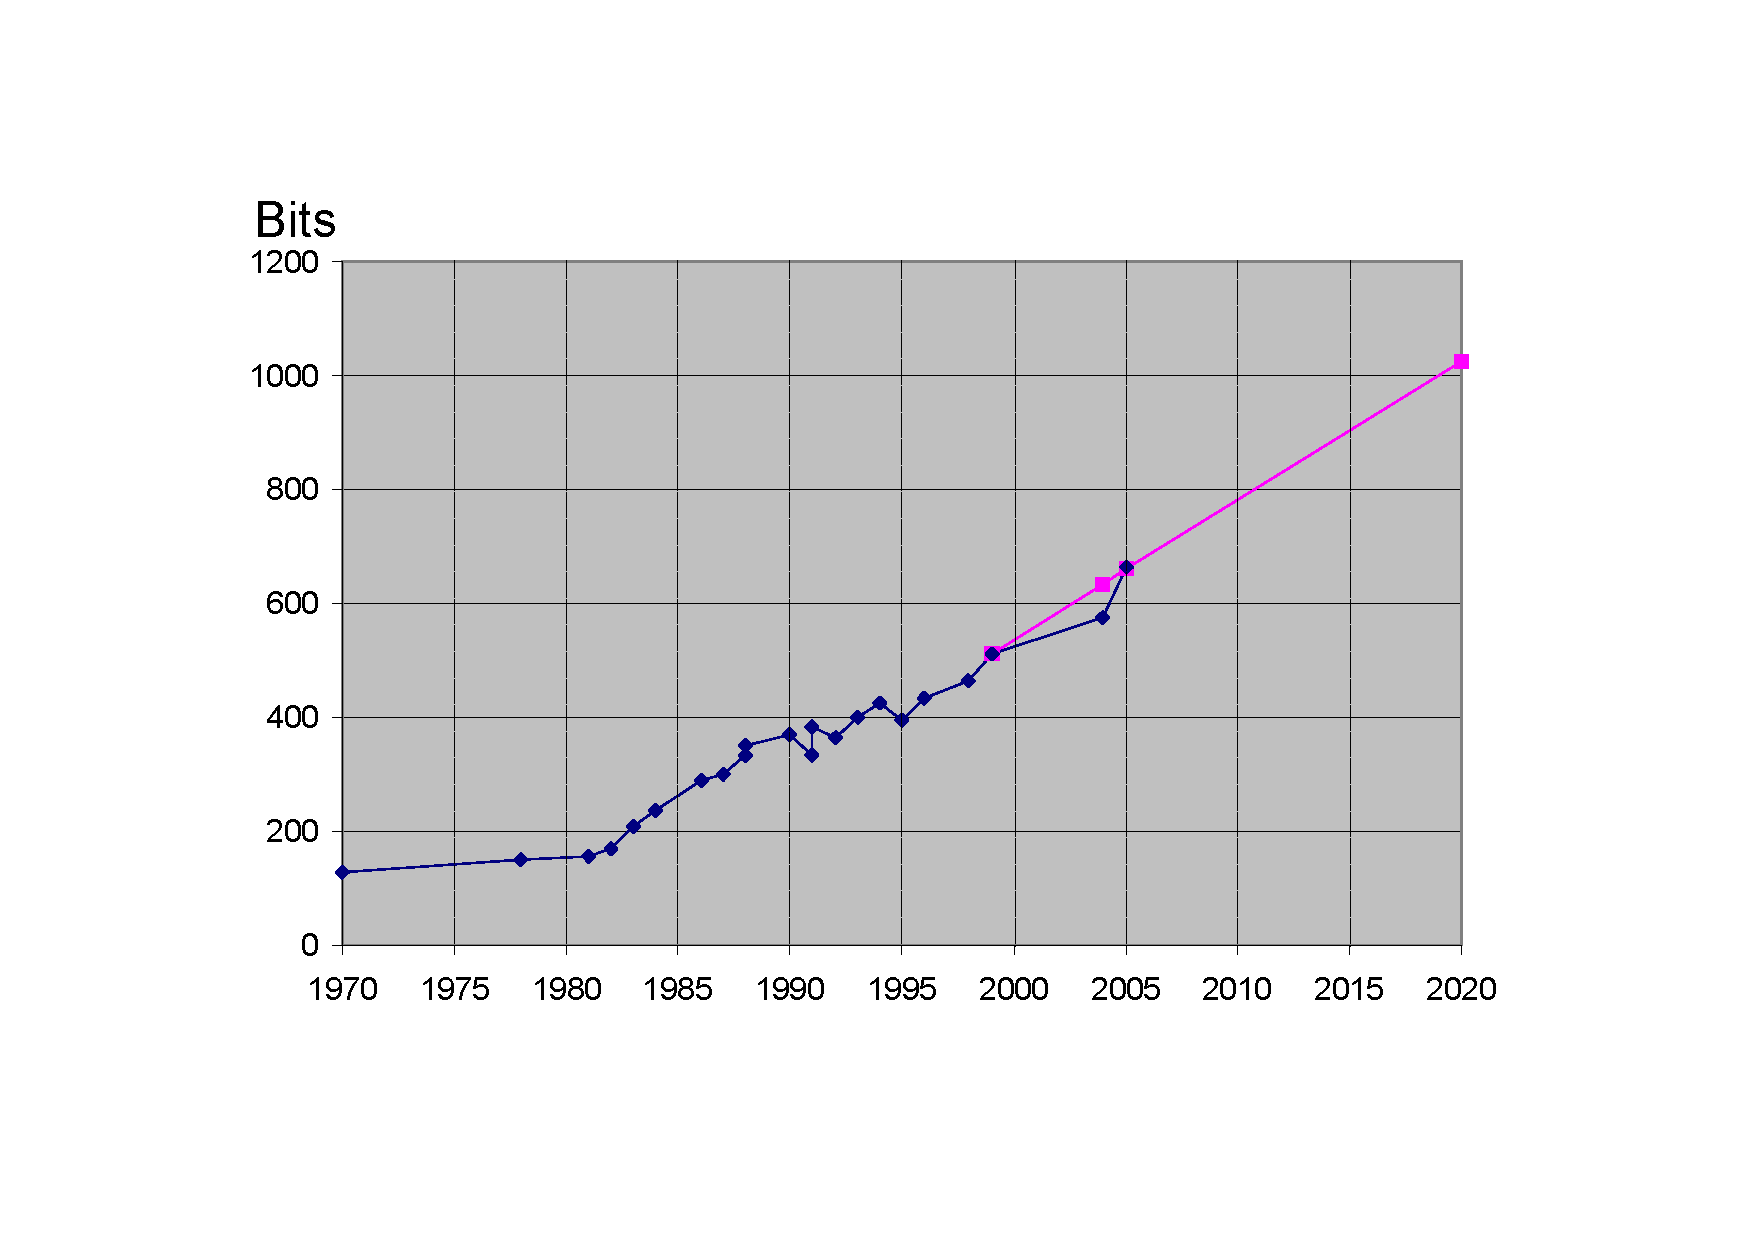
\includegraphics[scale=0.70, clip, viewport=50 20 700 430]{figures/PrognoseRSAFaktorisierungSecorvo.pdf}
%                                           links unten rechts oben
}
\caption{Vorhersage "uber die zuk"unftigen Faktorisierungsrekorde verglichen
mit aktuellen Resultaten (Quelle Secorvo)}
\label{secorvo-factorisation-forecast}
\end{center}
\end{figure}

%be_2005: Erzwingen, dass die Abb. noch in diesem Kapitel !





% ++++++++++++++++++++++++++++++++++++++++++++++++++++++++++++++++++++++++++
\vspace{6ex}
\begin{center}
\fbox{\parbox{15cm}{
    \emph{Hermann Hesse\footnotemark:}\\
    Damit das M"ogliche entsteht, muss immer wieder das Unm"ogliche 
    versucht werden.
}}
\end{center}
\addtocounter{footnote}{0}\footnotetext{%
    Hermann Hesse, deutsch-schweizerischer Schriftsteller und Nobelpreistr"ager, 
    02.07.1877$-$09.08.1962.}
% ++++++++++++++++++++++++++++++++++++++++++++++++++++++++++++++++++++++++++

\subsubsection{Status der Faktorisierung von konkreten gro"sen Zahlen}
\label{NoteFactorisation}

Ausf"uhrliche "Ubersichten "uber die Rekorde im Faktorisieren
zusammengesetzter Zahlen \index{Faktorisierung!Faktorisierungsrekorde}
mit unterschiedlichen Methoden finden sich auf den Webseiten 
\href{http://www.crypto-world.com}{\texttt{http://www.crypto-world.com}}
und
\href{http://www.tutorgig.com/ed/RSA\_number}{\texttt{http://www.tutorgig.com/ed/RSA\_number}}\footnote{%
Diese Seite war Ende Mai 2005 nicht ganz auf dem aktuellen Stand: RSA-200 fehlte.}. 

\vskip +10pt
Der aktuelle Rekord (Stand Mai 2005) mit der GNFS-Methode (General Number
Field Sieve) \index{General Number Field Sieve (GNFS)} liegt in der Zerlegung
einer $200$-stelligen Dezimalzahl in ihre beiden Primfaktoren.

\vskip +10pt
Die letzten Rekorde\footnote{%
Die  "`RSA-Zahlen"' sind gro"se semiprime Zahlen (d.h. Zahlen, die genau aus
2 Primfaktoren bestehen). Sie wurden von der Firma RSA Security generiert und 
ver"offentlicht, und sie bilden die "`RSA Factoring Challenge"': In diesem 
Wettbewerb werden die Primfaktoren dieser Zahlen gesucht.
Siehe \href{http://www.rsasecurity.com/rsalabs/challenges/factoring/numbers.html}
   {\texttt{http://www.rsasecurity.com/rsalabs/challenges/factoring/numbers.html}}.

In der ersten RSA-Factoring-Challenge wurden die Zahlen, von RSA-100 bis RSA-500, 
gem"a"s der Anzahl ihrer Dezimalstellen benannt; die zweite RSA-Factoring-Challenge 
benannte die Zahlen anhand der Anzahl ihrer Bin"arstellen. Innerhalb des zweiten 
Wettbewerbs sind Geldpreise f"ur die erfolgreiche Faktorisierung 
von RSA576 bis RSA2048 ausgelobt (RSA576, RSA640 etc. in 64-er Schritten).
Die Zahl RSA617 bildet eine Ausnahme, da sie vor der "Anderung des 
Namensschemas erzeugt wurde.

Die Forscher um Prof. Jens Franke (von der Universit"at Bonn, dem BSI und dem CWI) 
sind nicht auf die Geldpreise aus, sondern wollen die Grenzen der Forschung 
ausdehnen. Dadurch werden Aussagen "uber notwendige Minimall"angen f"ur 
sichere RSA-Moduli fundierter. 

Die "`C-Zahlen"' stammen aus dem Cunningham-Projekt:
\href{http://www.cerias.purdue.edu/homes/ssw/cun/}
     {\texttt{http://www.cerias.purdue.edu/homes/ssw/cun/}}
                                                               } 
mit Faktorisierungsverfahren f"ur zusammengesetzte Zahlen
sind in der folgenden Tabelle aufgef"uhrt:

\begin{table}[h]
\begin{center}
\begin{tabular}{|c|ccccc|}
\hline
   & {\bf Dezimalstellen} & {\bf Bin"arstellen} & & {\bf Faktorisiert am} & {\bf Faktorisiert von} \\
\hline
	RSA-155	&	155 & 512 & & August, 1999 & Herman te Riele et al. \\
	C158 & 		158 & 523 & & Januar, 2002 & Jens Franke et al. \\
	RSA-160 & 	160 & 530 & & April, 2003 & Jens Franke et al. \\
	RSA576 & 	174 & 576 & & Dezember, 2003 & Jens Franke et al. \\
	C176 & 		176 & 583 & & Mai, 2005 & Kazumaro Aoki et al. \\
	RSA-200 & 	200 & 663 & & Mai, 2005 & Jens Franke et al. \\
\hline
\end{tabular}
\caption{Die derzeitigen Faktorisierungsrekorde f"ur allgemeine Zahlen (Stand Mai 2005)}
\end{center}
\end{table}

%be_2005: Erzwingen, dass die Abb. noch in diesem Kapitel !


Im Folgenden werden diese letzten Rekorde etwas ausf"uhrlicher erl"autert.


% --------------------------------------------------------------------------
\vskip +20pt
\paragraph{RSA-155} \label{RSA-155} \index{RSA-155} 
\mbox{} % f"ur Zeilenumbruch, da er // allein nicht mag ! xxxxxxxxx

Am 22. Oktober 1999 fanden niederl"andische Forscher die L"osung dieser 
RSA-Challenge. Sie zerlegten eine $155$-stellige Zahl in ihre beiden $78$-stelligen
Primfaktoren (vergleiche Kapitel \ref{chptSecurityParam}).
Mit der $512$ Bit-Zahl RSA-155 war eine {\em magische} Grenze erreicht.



% --------------------------------------------------------------------------
\vskip +20pt
\paragraph{C158} \label{C158} \index{C158} 
\mbox{} % f"ur Zeilenumbruch, da er \\ allein nicht mag ! xxxxxxxxx
\hypertarget{C158-chap3}{}

Am 18. Januar 2002 zerlegten Forscher der Universit"at Bonn\footnote{%
\href{http://www.uni-bonn.de/Aktuelles/Pressemitteilungen/pm02/pm035-02.html}
{\texttt{http://www.uni-bonn.de/Aktuelles/Pressemitteilungen/pm02/pm035-02.html}}} 
mit der GNFS-Methode (General Number Field Sieve) \index{General Number
Field Sieve (GNFS)} eine $158$-stellige Dezimalzahl in ihre beiden Primfaktoren 
(diese haben 73 und 86 Dezimalstellen).

Dieser Rekord fand deutlich weniger Aufmerksamkeit in der Presse als die
L"osung von RSA-155.

Die Aufgabe der Bonner Wissenschaftler entsprang auch nicht einer Challenge,
sondern die Aufgabe war, die letzten Primfaktoren der Zahl $2^{953}+1$ 
zu finden (siehe~ ``Wanted List'' des Cunningham-Projekts\index{%
Cunningham-Projekt}\footnote{%
Cunningham-Projekt: \href{http://www.cerias.purdue.edu/homes/ssw/cun/}
                 {\texttt{http://www.cerias.purdue.edu/homes/ssw/cun/}}}). 

Die 6 kleineren, schon vorher gefundenen Primfaktoren dieser Zahl waren:
$$
\begin{array}{c}
        3, 1907, 425796183929, \\ 
        1624700279478894385598779655842584377, \\
        3802306738549441324432139091271828121 \quad{\rm und} \\ 
        128064886830166671444802576129115872060027.
\end{array}
$$
\begin{sloppypar}
Die drei kleinsten Faktoren k"onnen leicht\footnote{%
Z.B. mit CrypTool\index{CrypTool} "uber das Men"u 
{\bf Einzelverfahren \textbackslash{} RSA-Kryptosystem \textbackslash{} 
Faktorisieren einer Zahl}. \\
In sinnvoller Zeit zerlegt CrypTool Zahlen bis 250 Bit L"ange.
Zahlen gr"o"ser als 1024 Bit werden zur Zeit von CrypTool nicht angenommen.
}
bestimmt werden.
Die n"achsten drei Primfaktoren wurden von P.~Zimmerman%
\footnote{\href{http://www.loria.fr/zimmerma/ecmnet}{\tt http://www.loria.fr/\~{}zimmerma/ecmnet}}, 
T.~Grandlund%
\footnote{\href{http://www.swox.se/gmp/}{\tt http://www.swox.se/gmp/}}
und R. Harley in den Jahren 1999 und 2000 mit der Methode der Elliptischen
Kurven gefunden.
\end{sloppypar}

Als letzter Faktor blieb der sogenannte Teiler  "`C158"',
von dem man bis dahin wusste, dass er zusammengesetzt ist, aber man kannte
seine Primfaktoren nicht (die folgenden drei Zeilen sind eine einzige Zahl):
$$
\begin{array}{c}
39505874583265144526419767800614481996020776460304936 \\
45413937605157935562652945068360972784246821953509354 \\
4305870490251995655335710209799226484977949442955603
\end{array}
$$
Die Faktorisierung von C158 ergab die beiden 73- und 86-stelligen Primfaktoren:
$$
\begin{array}{c}
3388495837466721394368393204672181522815830368604993048084925840555281177
\end{array}
$$
und
$$
\begin{array}{c}
1165882340667125990314837655838327081813101 \\
2258146392600439520994131344334162924536139.
\end{array}
$$
Damit wurde die Zahl $2^{953}+1$ vollst"andig in ihre 8 Primfaktoren zerlegt.

\begin{minipage}{\textwidth}
\vspace{3ex}
Verweise:
\vspace{-10pt}
\begin{itemize}
\item[]   \href{http://www.loria.fr/\~{}zimmerma/records/gnfs158}
       {\texttt{http://www.loria.fr/\~{}zimmerma/records/gnfs158}} \\
          \href{http://www.crypto-world.com/FactorRecords.html}
       {\texttt{http://www.crypto-world.com/FactorRecords.html}} \\
          \href{http://www.crypto-world.com/announcements/c158.txt}
       {\texttt{http://www.crypto-world.com/announcements/c158.txt}}
\end{itemize}
\end{minipage}



% --------------------------------------------------------------------------
\vskip +20pt
\paragraph{RSA-160} \label{RSA-160} \index{RSA-160}\mbox{}
\hypertarget{RSA-160-chap3}{}

Am 1. April 2003 zerlegten Forscher der Universit"at Bonn\footnote{%
          \href{http://www.loria.fr/~zimmerma/records/rsa160}
       {\texttt{http://www.loria.fr/\~{}zimmerma/records/rsa160}} \\
          \href{http://www.loria.fr/~zimmerma/records/factor.html}
       {\texttt{http://www.loria.fr/\~{}zimmerma/records/factor.html}} \\
          \href{http://www.crypto-world.com/FactorWorld.html}
       {\texttt{http://www.crypto-world.com/FactorWorld.html}}
} 
mit der GNFS-Methode (General Number Field Sieve) \index{General Number
Field Sieve (GNFS)} eine $160$-stellige Zahl in ihre beiden Primfaktoren 
(diese haben jeweils 80 Dezimalstellen).

Die Berechnungen dazu fanden auch im Bundesamt f"ur Sicherheit in der 
Informationstechnik (BSI) in Bonn statt\footnote{%
Das BSI \index{BSI} erstellt jedes Jahr ein Papier "uber die Eignung von
Kryptoalgorithmen, mit denen Signaturen erzeugt werden k"onnen,         
die den Vorgaben des deutschen Signaturgesetzes gen"ugen.
Bei dieser Erstellung werden Experten aus Wirtschaft und Wissenschaft
beteiligt. Um die Eignung von Signaturverfahren zu beurteilen, deren
Schwierigkeit auf dem Faktorisierungsproblem beruht,
kooperiert das BSI auch mit Forschern der Universit"at Bonn.
Weitere Informationen zu Kryptoalgorithmen finden Sie auf den BSI-Internetseiten unter:
   \href{http://www.bsi.bund.de/esig/basics/techbas/krypto/index.htm}
{\texttt{http://www.bsi.bund.de/esig/basics/techbas/krypto/index.htm}}
}.

Die 160-stellige Dezimalzahl stammt von der alten Challenge-Liste von RSADSI.
Diese wurde nach der Faktorisierung von RSA-155 (RSA512) zur"uckgezogen.
Die Primfaktoren von RSA-160 waren aber nicht bekannt.
Deshalb ist dieser Rekord von Prof.\ Frankes Team immer noch die L"osung 
einer alten Challenge, f"ur die es aber von RSADSI kein Geld gibt.

Die zusammengesetzte Zahl "`RSA-160"' lautet (die folgenden drei Zeilen 
sind eine einzige Zahl):
$$
\begin{array}{c}
215274110271888970189601520131282542925777358884567598017049 \\
767677813314521885913567301105977349105960249790711158521430 \\
2079314665202840140619946994927570407753
\end{array}
$$
Die Faktorisierung von RSA-160 ergab die beiden Primfaktoren:
$$
\begin{array}{c}
p = 45427892858481394071686190649738831 \\         
    656137145778469793250959984709250004157335359
\end{array}
$$
und
$$
\begin{array}{c}
q = 47388090603832016196633832303788951 \\
    973268922921040957944741354648812028493909367
\end{array}
$$

Die Berechnungen erfolgten zwischen Dezember 2002 und April 2003.
\vspace{24pt}



% ammmmmmmmmmma
% 
% RSA-576 faktorisiert 
% Am 27.04.2004 ging die Nachricht durch
% die Ticker, dass die 576-bit-Challenge der
% Firma RSA gel�st sei. Tats�chlich wurde
% die 174 Dezimalstellen lange Zahl bereits
% am 03.12.2003 zerlegt. Die Faktorisierung
% gelang einem Team der Universit�t Bonn
% um Professor Franke mit Unterst�tzung
% durch das Institut f�r Experimentelle Mathematik
% in Essen und das BSI. Die verteilte
% Berechung erfolge auf einem Linux-
% Cluster mit 144 PCs (400 MHz, Pentium II)
% und verwendete den General Number Field
% Sieve-Algorithmus ? mit einem Aufwand
% von umgerechnet 13.200 MIPS-Jahren.
% Interessant dabei: Dieser Faktorisierungserfolg
% best�tigt die Prognose, die Secorvo
% vor drei Jahren auf der Basis der Faktorisierungserfolge
% der vergangenen 30 Jahre
% gestellt hat (siehe Bild), und die weit weniger
% dramatisch ausfiel als viele Expertenwarnungen
% und die Erwartung des BSI.
% Danach w�re 2004 erstmals die Faktorisierung
% einer 630 bit langen Zahl zu erwarten
% gewesen ? was nun eher unwahrscheinlich
% erscheint. Selbst die fr�hestens f�r das
% Jahr 2020 vorausgesagte Faktorisierung
% eines 1024 bit langen RSA-Schl�ssels
% k�nnte sich daher noch als zu pessimistische
% Bef�rchtung erweisen ? allen Warnern
% zum Trotz, die seit Jahren Schl�ssell
% �ngen von 2048 bit und mehr empfehlen
% oder gar das baldige Ende von RSA prophezeihen.
% 
% ammmmmmmmmmmz




% --------------------------------------------------------------------------
\vskip +20pt
\paragraph{RSA-200} \label{RSA-200} \index{RSA-200}\mbox{}
\hypertarget{RSA-200-chap3}{}

Am 9. Mai 2005 meldete die Forschergruppe von Prof. Jens Franke der Universit"at Bonn\footnote{%
   \href{http://www.loria.fr/~zimmerma/records/rsa200}
{\texttt{http://www.loria.fr/\~{}zimmerma/records/rsa200}}}, dass sie
gemeinsam mit Kollegen des Amsterdam Centrum voor Wiskunde en Informatica
einen neuen Weltrekord im Faktorisieren aufstellten. 

Sie zerlegten mit der GNFS-Methode (General Number Field Sieve) \index{General Number
Field Sieve (GNFS)} eine $200$-stellige Zahl in ihre beiden Primfaktoren 
(diese haben jeweils 100 Dezimalstellen).

Die zusammengesetzte Zahl "`RSA-200"' lautet (die folgenden drei Zeilen 
sind eine einzige Zahl):
$$
\begin{array}{c}
2799783391122132787082946763872260162107044678695542853756000992932 \\
6128400107609345671052955360856061822351910951365788637105954482006 \\
576775098580557613579098734950144178863178946295187237869221823983
\end{array}
$$
Die Faktorisierung von RSA-200 ergab die beiden Primfaktoren:
$$
\begin{array}{c}
p = 35324619344027701212726049781984643686711974001976 \\         
    25023649303468776121253679423200058547956528088349
\end{array}
$$
und
$$
\begin{array}{c}
q = 79258699544783330333470858414800596877379758573642 \\
    19960734330341455767872818152135381409304740185467
\end{array}
$$

Die Berechnungen erfolgten zwischen Dezember 2003 und Mai 2005.
Die Faktorisierung durch die Gruppe um Bahr, B"ohm, Franke, Kleinjung, 
Montgomery und te Riele hatte also knapp 17 Monate gedauert.
Der Rechenaufwand lag bei umgerechnet etwa 120.000 MIPS-Jahren\footnote{%
Ein MIPS-Jahr (MY) ist die Anzahl von Operationen, die eine Maschine, 
welche eine Million Integeroperationen pro Sekunde (MIPS)
ausf"uhrt, in einem Jahr bew"altigt. Zur Illustration: ein INTEL 
Pentium 100 Prozessor hat etwa 50 MIPS.
F"ur die Zerlegung eines 2048-Bit-Moduls br"auchte man ca. {$8,5 \cdot 
10^{40}$ MY}.}.




% --------------------------------------------------------------------------
\vskip +50pt
\paragraph{Gr"o"senordnung faktorisierter Zahlen im Vergleich zu auf Primalit"at getesteter Zahlen}
\mbox{}

Wie man sieht, sind die gr"o"sten (aus 2 Primfaktoren) zusammengesetzten Zahlen,
die man faktorisieren kann, deutlich kleiner als die Zahlen mit einer 
speziellen Struktur, f"ur die Primzahltests\index{Primzahltest} in der Lage
sind, Aussagen "uber ihre Primalit"at zu treffen (siehe Kapitel 
\ref{search_for_very_big_primes}, \ref{primality_tests} und
\ref{spezialzahlentypen}).


% be_2005_UPDATEN_if-new-mersenne-prime-appears

L"ange in Bit der derzeitigen Weltrekorde (RSA-200 $\longleftrightarrow{}$ M-42):
  ~  $663 \longleftrightarrow{} 25.964.951$.

%be_2005 - erzwungenes Blank und $$ um Pfeilzeichen, sonst setzt er Blanks an 
%          die falschen Stellen.
%        - Wenn man hier \~ statt nur ~ (au�erhalb der $$) schreibt, kommen
%          nachher Fussnoten mit {\bf Einzelverfahren \textbackslash{} Protokolle}
%          nur noch mit kaputten Schriftzeichen raus !



% --------------------------------------------------------------------------
\vskip +60pt
\subsubsection{Weitere aktuelle Forschungsergebnisse zu Primzahlen und Faktorisierung}
Primzahlen sind Teil vieler hochaktueller Forschungsgebiete der Zahlentheorie. 
Die Fortschritte bei der Faktorisierung sind gr"o"s als noch vor 5 Jahren
gesch"atzt -- sie gehen nicht nur auf das Konto schnellerer Rechner, 
sondern sie sind auch in neuen Erkenntnissen begr"undet.

Die Sicherheit des RSA-Algorithmus basiert auf der empirischen Beobachtung, dass die Faktorisierung gro"ser ganzer 
Zahlen ein schwieriges Problem ist. Besteht wie beim RSA-Algorithmus der zugrunde liegende Modul $n$ aus dem Produkt 
zweier gro"ser Primzahlen $p, q$ (typische L"angen: $p, q$  $500-600$ bit, $n$ $1024$ bit), so l"asst sich 
$n=pq$ aus $p$ und $q$ leicht bestimmen, jedoch ist es mit den bisher bekannten Faktorisierungsalgorithmen nicht
m"oglich, $p, q$ aus $n$ zu gewinnen. Nur mit Kenntnis von $p$ und $q$ l"asst sich jedoch der private aus dem 
"offentlichen Schl"ussel ermitteln.

Die Entdeckung eines Algorithmus zur effizienten Faktorisierung von Produkten $n=pq$ gro"ser Primzahlen w"urde daher 
den RSA-Algorithmus wesentlich beeintr"achtigen. Je nach Effizienz der Faktorisierung im Vergleich zur Erzeugung von 
$p, q, n$ m"usste der verwendete Modul $n$ (z.Zt. 1024 bit) erheblich vergr"o"sert oder --- im Extremfall --- auf den 
Einsatz des RSA ganz verzichtet werden.


% --------------------------------------------------------------------------
\vskip +20pt
\paragraph{Das Papier von Bernstein und seine Auswirkungen auf die Sicherheit
des RSA-Algorithmus} \label{RSABernstein} \index{Faktorisierung!Faktorisierungsproblem}
\mbox{} % f"ur Zeilenumbruch, da er \\ allein nicht mag ! 
        % Braucht die Leerzeile danach auch noch !! bebebe ?

Die im November 2001 ver"offentlichte Arbeit ``Circuits for integer
factorization: a proposal'' (siehe
\href{http://cr.yp.to/djb.html}{\texttt{http://cr.yp.to/djb.html}}) von
D.J. Bernstein \cite{Bernstein2001} behandelt das Problem der 
Faktorisierung gro"ser Zahlen.
Die Kernaussage des Papers besteht darin, dass es m"oglich ist, die
Implementierung des General Number Field Sieve-Algorithmus (GNFS)
\index{General Number Field Sieve (GNFS)} so zu
verbessern, dass mit gleichem Aufwand wie bisher Zahlen mit 3-mal
gr"o"serer Stellenzahl (Bit-L"ange) faktorisiert werden k"onnen.

Wesentlich bei der Interpretation des Resultats ist die Definition des
Aufwandes: Als Aufwand wird das Produkt von ben"otigter Rechenzeit und
Kosten der Maschine (insbesondere des verwendeten Speicherplatzes)
angesetzt. Zentral f"ur das Ergebnis des Papiers ist die Beobachtung, dass
ein wesentlicher Teil der Faktorisierung auf Sortierung zur"uckgef"uhrt
werden kann und mit dem Schimmlerschen Sortierschema ein Algorithmus zur
Verf"ugung steht, der sich besonders gut f"ur den Einsatz von
Parallelrechnern eignet. Am Ende des Abschnittes 3 gibt Bernstein konkret
an, dass die Verwendung von $m^2$ Parallelrechnern mit jeweils gleicher
Menge an Speicherplatz mit Kosten in der Gr"o"senordnung von $m^2$
einhergeht --- genau so wie ein einzelner Rechner mit $m^2$ Speicherzellen.
Der Parallelrechner bew"altigt die Sortierung von $m^2$ Zahlen jedoch
(unter Verwendung der o.~g.\ Sortierverfahrens) in Zeit proportional zu m,
wohingegen der Einprozessorrechner Zeit proportional $m^2$ ben"otigt.
Verringert man daher den verwendeten Speicherplatz und erh"oht --- bei
insgesamt gleich bleibenden Kosten --- die Anzahl der Prozessoren
entsprechend, verringert sich die ben"otigte Zeit um die Gr"o"senordnung
$1/m$. In Abschnitt 5 wird ferner angef"uhrt, dass der massive Einsatz der
parallelisierten Elliptic Curve-Methode von Lenstra die Kosten der
Faktorisierung ebenfalls um eine Gr"o"senordnung verringert (ein
Suchalgorithmus hat dann quadratische statt kubische Kosten).  Alle
Ergebnisse von Bernstein gelten nur asymptotisch f"ur gro"se Zahlen $n$.
Leider liegen keine Absch"atzungen "uber den Fehlerterm, d.h.  die
Abweichung der tats"achlichen Zeit von dem asymptotischen Wert, vor --- ein
Mangel, den auch Bernstein in seinem Papier erw"ahnt. Daher kann zur Zeit
keine Aussage getroffen werden, ob die Kosten (im Sinne der Bernsteinschen
Definition) bei der Faktorisierung z.~Zt.\ verwendeter RSA-Zahlen
(1024$-$2048 bit) bereits signifikant sinken w"urden.

Zusammenfassend l"asst sich sagen, dass der Ansatz von Bernstein durchaus 
innovativ ist. Da die Verbesserung der 
Rechenzeit unter gleichbleibenden Kosten durch einen massiven Einsatz von 
Parallelrechnern erkauft wird, stellt sich die 
Frage nach der praktischen Relevanz. Auch wenn formal der Einsatz von einem 
Rechner "uber 1 sec  und  1.000.000 Rechnern 
f"ur je 1/1.000.000 sec dieselben Kosten erzeugen mag, ist die 
Parallelschaltung von 1.000.000 Rechnern praktisch nicht 
(oder nur unter immensen Fixkosten, insbesondere f"ur die Vernetzung der
Prozessoren) zu realisieren. Solche Fixkosten 
werden aber nicht in Ansatz gebracht.
Die Verwendung verteilter Ans"atze (distributed computing) "uber ein 
gro"ses Netzwerk k"onnte einen Ausweg bieten. Auch hier m"ussten  
Zeiten und Kosten f"ur Daten"ubertragung einkalkuliert werden.

Solange noch keine (kosteng"unstige) Hardware oder verteilte Ans"atze 
entwickelt wurden, die auf 
dem Bernsteinschen Prinzip basieren, besteht noch keine akute Gef"ahrdung
des RSA. Es bleibt zu kl"aren, ab welchen 
Gr"o"senordnungen von n die Asymptotik greift. 

Arjen Lenstra, Adi Shamir et.~al.\ haben das Bernstein-Paper analysiert 
\cite{Lenstra2002}.
Als Ergebnis kommen Sie zu einer Bitl"angen-Verbesserung der 
Faktorisierung um den Faktor 1.17 
(anstatt Faktor 3 wie von Bernstein erwartet).

Die Zusammenfassung ihres Papers ``Analysis of Bernstein's Factorization 
Circuit'' lautet:

``... Bernstein proposed a circuit-based implementation of
the matrix step of the number field sieve factorization algorithm. We
show that under the non-standard cost function used in [1], these circuits
indeed offer an asymptotic improvement over other methods but
to a lesser degree than previously claimed: for a given cost, the new
method can factor integers that are 1.17 times larger (rather than 3.01).
We also propose an improved circuit design based on a new mesh routing
algorithm, and show that for factorization of 1024-bit integers the
matrix step can, under an optimistic assumption about the matrix size,
be completed within a day by a device that costs a few thousand dollars.
We conclude that from a practical standpoint, the security of RSA relies
exclusively on the hardness of the relation collection step of the number
field sieve.''

Auch \href{http://www.rsasecurity.com/}{RSA Security} kommt in ihrer Analyse der Bernstein-Arbeit \cite{RSA Security 2002} vom 8. April 2002 erwartungsgem"a"s
zu dem Ergebnis, dass RSA weiterhin als ungebrochen betrachtet werden kann.

Die Diskussion ist weiterhin im Gang.

Zum Zeitpunkt der Erstellung dieses Absatzes (Juni 2002) war nichts
dar"uber bekannt, inwieweit die im Bernstein-Papier vorgeschlagenen
theoretischen Ans"atze realisiert wurden oder wieweit die Finanzierung
seines Forschungsprojektes ist.

\begin{minipage}{\textwidth}
\vspace{3ex}
Verweise:
\vspace{-10pt}
\begin{itemize}
  \item[] \href{http://cr.yp.to/djb.html}
               {\texttt{http://cr.yp.to/djb.html}} \\
          \href{http://www.counterpane.com/crypto-gram-0203.html\#6}
               {\texttt{http://www.counterpane.com/crypto-gram-0203.html\#6}} \\
          \href{http://www.math.uic.edu}
               {\texttt{http://www.math.uic.edu}} 
\end{itemize}
\end{minipage}



% --------------------------------------------------------------------------
\vskip +20pt
\paragraph{Das TWIRL-Device} \label{TWIRLDevice} \index{TWIRL-Device}
\mbox{} % f"ur Zeilenumbruch, da er // allein nicht mag ! xxxxxxxxx

Im Januar 2003 ver"offentlichten Adi Shamir und Eran Tromer vom Weizmann Institute of Science den vorl"aufigen Draft {\em ``Factoring Large Numbers with the TWIRL Device''}, in dem deutliche Bedenken gegen RSA-Schl"ussell"angen unter 1024 begr"undet werden \cite{Shamir2003}.

Das Abstract fasst ihre Ergebnisse folgenderma"sen zusammen: ``The security of the RSA cryptosystem depends on the difficulty of factoring large integers. The best current factoring algorithm is the Number Field Sieve (NFS), and its most difficult part is the sieving step. In 1999 a large distributed computation involving thousands of workstations working for many months managed to factor a 512-bit RSA key, but 1024-bit keys were believed to be safe for the next 15-20 years. In this paper we describe a new hardware implementation of the NFS sieving step ... which is 3-4 orders of magnitude more cost effective than the best previously published designs ... . Based on a detailed analysis of all the critical components (but without an actual implementation), we believe that the NFS sieving step for 1024-bit RSA keys can be completed in less than a year by a \$10M device, and that the NFS sieving step for 512-bit RSA keys can be completed in less than ten minutes by a \$10K device. Coupled with recent results about the difficulty of the NFS matrix step ... this raises some concerns about the security of these key sizes.''

Eine sehr gute Erl"auterung, wie der Angriff mit dem Generalized Number Field
Sieve (GNFS) \index{General Number Field Sieve (GNFS)} funktioniert und
welche Fortschritte sich ergaben, findet sich
in dem 3-seitigen Artikel in der DuD-Ausgabe Juni/2003 \cite{Weis2003}.
Beim GNFS k"onnen 2 grundlegende Schritte unterschieden werden: 
der Siebungsschritt (Relationen sammeln) und die Matrix-Reduktion.
Auch wenn der Siebungsschritt hochgradig parallelisierbar ist, so dominiert
er doch den Gesamtrechenaufwand. Bisher haben Shamir und Tromer noch kein 
TWIRL-Device gebaut, jedoch ist der daf"ur gesch"atzte Aufwand von 10 bis
50 Millionen Euro, um eine 1024-Bit Zahl in einem Jahr zu faktorisieren
f"ur Geheimdienste oder gro"se kriminelle Organisationen keineswegs prohibitiv,
denn die \glqq Kosten f"ur einen einzigen Spionagesatelliten sch"atzt man
z.B. auf mehrere Milliarden USD\grqq. Die Autoren empfehlen deshalb konkret,
m"oglichst rasch sensible, bisher benutzte RSA-, Diffie-Hellman- oder 
ElGamal-Schl"ussel von bis zu 1024 Bit zu wechseln und Schl"ussel von 
mindestens 2048 Bit L"ange einzusetzen.
Auch f"ur die geplante TCPA/Palladium-Hardware \index{Palladium} werden
2048-Bit RSA-Schl"ussel verwendet!

Damit erscheinen die aktuellen Empfehlungen des BSI, auf l"angere RSA-Schl"ussell"angen umzustellen, mehr als gerechtfertigt.



% --------------------------------------------------------------------------
\vskip +20pt
\paragraph{``Primes in P'': Testen auf Primalit"at ist polynominal} \label{PrimesinP} \index{Primzahltest} 
\mbox{} % f"ur Zeilenumbruch, da er // allein nicht mag ! xxxxxxxxx

Im August 2002 ver"offentlichten die drei indischen Forscher M. Agrawal, N. Kayal und N. Saxena ihr Paper {\em ``PRIMES in P''} "uber einen neuen Primzahltest-Algorithmus, genannt AKS\index{AKS} \cite{Agrawal2002}. 
Sie entdeckten einen polynominalen\index{Polynom} deterministischen Algorithmus, um zu entscheiden, ob eine gegebene Zahl prim ist oder nicht.

Die Bedeutung dieser Entdeckung liegt darin, dass sie Zahlentheoretiker mit neuen Einsichten und M"oglichkeiten f"ur die weitere Forschung versorgt. Viele Menschen haben im Lauf der Jahrhunderte nach einem polynominalen Primzahltest gesucht, so dass dieses Ergebnis einen theoretischen Durchbruch darstellt. Es zeigt sich immer wieder, dass aus schon lange bekannten Fakten neue Ergebnisse generiert werden k"onnen.

Aber selbst die Autoren merken an, dass andere bekannte Algorithmen (z.B. ECPP) schneller sein k"onnen. Der neue Algorithmus funktioniert f"ur alle positiven ganzen Zahlen. Dagegen verwendet das GIMPS-Projekt den Lucas-Lehmer-Primzahltest, der besondere Eigenschaften der Mersennezahlen ausnutzt. Dadurch ist der Lucas-Lehmer-Test viel schneller und erlaubt, Zahlen mit Millionen von Stellen zu testen, w"ahrend generische Algorithmen auf Zahlen mit einigen tausend Stellen beschr"ankt sind. Nachteil der bisherigen schnellen Verfahren ist, dass sie probabilistisch sind, also ihr Ergebnis h"ochstwahrscheinlich, aber nicht ganz sicher ist.

\enlargethispage{20pt}
Aktuelle Forschungsergebnisse dazu finden sich z.B. auf: 
\vspace{-10pt}
\begin{itemize}
  \item[] \href{http://www.mersenne.org/}
               {\texttt{http://www.mersenne.org/}} \\
          \href{http://fatphil.org/maths/AKS/}
               {\texttt{http://fatphil.org/maths/AKS/}} Originaltext in Englisch\\
          \href{http://ls2-www.cs.uni-dortmund.de/lehre/winter200203/kt/material/primes.ps}
               {\texttt{http://ls2-www.cs.uni-dortmund.de/lehre/winter200203/kt/material/primes.ps}}\\\hspace*{2em}Gute Erl"auterung in Deutsch von Thomas Hofmeister.
\end{itemize}

\vskip +10 pt




% ++++++++++++++++++++++++++++++++++++++++++++++++++++++++++++++++++++++++++
\newpage
\begin{center}
\fbox{\parbox{15cm}{{\em Joanne K.\index{Rowling, Joanne} Rowling\footnotemark:}\newline
Viel mehr als unsere F"ahigkeiten sind es 
unsere Entscheidungen ..., die zeigen, wer wir wirklich sind.}}
\end{center}

\addtocounter{footnote}{0}\footnotetext{Joanne K. Rowling, \glqq Harry Potter und die Kammer des Schreckens'', Carlsen,
(c) 1998, letztes Kapitel \glqq Dobbys Belohnung'', S. 343, Dumbledore.}
% ++++++++++++++++++++++++++++++++++++++++++++++++++++++++++++++++++++++++++
\subsection{Anwendungen der asymmetrischen Kryptographie mit Zahlenbeispielen}

In der modernen Kryptographie \index{Kryptographie!moderne} werden die Ergebnisse der modularen Arithmetik
extensiv angewandt. Hier werden exemplarisch einige wenige Beispiele aus der
Kryptographie mit kleinen\footnote{%
\glqq Klein'' bedeutet beim RSA-Verfahren, dass die 
Bitl"angen der Zahlen sehr viel kleiner sind als $1024$ Bit (das sind $308$ Dezimalstellen). 
$1024$ Bit gilt im Moment in der Praxis als Mindestl"ange f"ur einen sicheren Certification
Authority-RSA-Modul.
} Zahlen vorgestellt.

Die Chiffrierung eines Textes besteht darin, dass man aus einer Zeichenkette
(Zahl) durch Anwenden einer Funktion (mathematische Operationen) eine andere
Zahl erzeugt. Dechiffrieren hei"st, diese Funktion umzukehren: aus dem
Zerrbild, das die Funktion aus dem Klartext gemacht hat, das Urbild
wiederherzustellen. Beispielsweise k"onnte der Absender einer vertraulichen
Nachricht zum Klartext $M$ eine geheimzuhaltende Zahl, den Schl"ussel $S$,
addieren und dadurch den Chiffretext $C$ erhalten:
$$ C = M + S. $$
Durch Umkehren dieser Operation, das hei"st durch Subtrahieren von $S$, kann
der Empf"anger den Klartext rekonstruieren:
$$ M = C - S. $$
Das Addieren von $S$ macht den Klartext zuverl"assig unkenntlich. Gleichwohl
ist diese Verschl"usselung sehr schwach; denn wenn ein Abh"orer auch nur ein
zusammengeh"origes Paar von Klar- und Chiffretext in die H"ande bekommt, kann
er den Schl"ussel berechnen
$$ S = C - M, $$
und alle folgenden mit $S$ verschl"usselten Nachrichten mitlesen. \\
Der wesentliche Grund ist, dass Subtrahieren eine ebenso einfache Operation
ist wie Addieren. 



% --------------------------------------------------------------------------
\subsubsection{Einwegfunktionen}
\hypertarget{OneWayFunktion2}{}%    %%% be_24.5.03 Ohne das % bg. die ff. Zeile ("Wenn der ...") mit einem Blank
Wenn der Schl"ussel auch bei gleichzeitiger Kenntnis von
Klar- und Chiffretext nicht ermittelbar sein soll, braucht man eine
Funktion, die einerseits relativ einfach berechenbar ist - man will ja
chiffrieren k"onnen. Andererseits soll ihre Umkehrung zwar existieren (sonst
w"urde beim Chiffrieren Information verlorengehen), aber de facto
unberechenbar sein.

Was sind denkbare Kandidaten f"ur eine solche\index{Einwegfunktion} {\bf Einwegfunktion}?
Man k"onnte an
die Stelle der Addition die Multiplikation setzen; aber schon Grundsch"uler
wissen, dass deren Umkehrung, die Division, nur geringf"ugig m"uhsamer ist als
die Multiplikation selbst. Man muss noch eine Stufe h"oher in der Hierarchie
der Rechenarten gehen: Potenzieren ist immer noch eine relativ einfache
Operation; aber ihre beiden Umkehrungen {\em Wurzelziehen} (finde $b$ in der
Gleichung $a = b^c$ , wenn $a$ und $c$ bekannt sind) und {\em Logarithmieren} (in
derselben Gleichung finde $c$, wenn $a$ und $b$ bekannt sind) sind so kompliziert,
dass ihre Ausf"uhrung in der Schule normalerweise nicht mehr gelehrt wird.

W"ahrend bei Addition und Multiplikation noch eine gewisse Struktur
wiedererkennbar ist, wirbeln Potenzierung und Exponentiation alle Zahlen
wild durcheinander: Wenn man einige wenige Funktionswerte kennt, wei"s man
(anders als bei Addition und Multiplikation) noch kaum etwas "uber die
Funktion im ganzen.



% --------------------------------------------------------------------------
\subsubsection{Das Diffie-Hellman Schl"usselaustausch-Protokoll 
               (Key Exchange Protocol)} 
\index{Diffie, Whitfield} 
\index{Hellman, Martin} 
\index{Schl""usselaustausch!Diffie-Hellman}
\index{Diffie-Hellman}

Das DH-Schl"usselaustauschprotokoll wurde 1976 in Stanford von Whitfield
Diffie, Martin E. Hellman und Ralph Merkle erdacht\footnote{%
  In CrypTool\index{CrypTool} ist dieses Austauschprotokoll visualisiert:
  Sie k"onnen die einzelnen Schritte mit konkreten Zahlen nachvollziehen 
  per Men"u {\bf Einzelverfahren \textbackslash{} Protokolle
           \textbackslash{} Diffie-Hellman-Demo}.
}. 

Eine Einwegfunktion dient Alice und Bob\footnote{%
Alice und Bob werden standardm"a"sig als die beiden berechtigten Teilnehmer
eines Protokolls bezeichnet (siehe \cite[Seite 23]{Schneier1996nt}).
} dazu, sich einen Schl"ussel $S$, den Sessionkey, f"ur die nachfolgende
Verst"andigung zu verschaffen. Dieser ist dann ein Geheimnis, das nur diesen
beiden bekannt ist. Alice w"ahlt sich eine Zufallszahl $a$ und h"alt sie geheim.
Aus $a$ berechnet sie mit der Einwegfunktion die Zahl $A = g^a$ und schickt sie
an Bob. Der verf"ahrt ebenso, indem er eine geheime Zufallszahl $b$ w"ahlt,
daraus $B = g^b$ berechnet und an Alice schickt. Die Zahl $g$ ist beliebig und
darf "offentlich bekannt sein. Alice wendet die Einwegfunktion mit ihrer
Geheimzahl $a$ auf $B$ an, Bob tut gleiches mit seiner Geheimzahl $b$ und der
empfangenen Zahl $A$.

Das Ergebnis $S$ ist in beiden F"allen dasselbe, weil die Einwegfunktion
kommutativ ist: $g^{a*b} = g^{b*a}$. Aber selbst Bob kann Alices Geheimnis $a$ nicht aus
den ihm vorliegenden Daten rekonstruieren, Alice wiederum Bobs Geheimnis $b$
nicht ermitteln, und ein Lauscher, der $g$ kennt und sowohl $A$ als auch $B$
mitgelesen hat, vermag daraus weder $a$ noch $b$ noch $S$ zu berechnen.

\vskip +10 pt
\input{figures/DH-de.latex}
\vskip +10 pt

{\bf Ablauf:}\par
Alice und Bob wollen also einen geheimen Sessionkey $S$ "uber einen
abh"orbaren Kanal aushandeln.
\begin{itemize}
   \item[\bf 1.] Sie w"ahlen eine Primzahl $p$ und eine Zufallszahl $g$, und tauschen diese
                 Information offen aus.
   \item[\bf 2.] Alice w"ahlt nun $a$, eine Zufallszahl kleiner $p$ und h"alt diese geheim.

                 Bob w"ahlt ebenso $b$, eine Zufallszahl kleiner $p$ und h"alt diese geheim.
   \item[\bf 3.] Alice berechnet nun $A \equiv g^a {\rm ~(mod~} p)$. \\
                 Bob berechnet $B \equiv g^b {\rm ~(mod~} p)$.
   \item[\bf 4.] Alice sendet das Ergebnis $A$ an Bob. \\
                 Bob sendet das Ergebnis $B$ an Alice.
   \item[\bf 5.] Um den nun gemeinsam zu benutzenden Sessionkey zu bestimmen, potenzieren sie
                 beide jeweils f"ur sich das jeweils empfangene Ergebnis mit ihrer geheimen
                 Zufallszahl modulo $p$. Das hei"st:
         \begin{itemize}
                    \item[-] Alice berechnet $S \equiv B^a {\rm ~(mod~} p)$, und 
                    \item[-] Bob berechnet   $S \equiv A^b {\rm ~(mod~} p)$.
         \end{itemize}
\end{itemize}       
Auch wenn ein Spion $g, p$, und die Zwischenergebnisse $A$ und $B$ abh"ort, kann er den 
schlie"slich bestimmten Sessionkey, wegen der Schwierigkeit, den diskreten Logarithmus zu \index{Logarithmusproblem!diskret}
bestimmen, nicht berechnen.

\vskip +10 pt
Das ganze soll an einem Beispiel mit (unrealistisch) kleinen Zahlen gezeigt
werden.\vskip +1em

{\bf Beispiel in Zahlen:} 
\begin{itemize}
   \item[\bf 1.] Alice und Bob w"ahlen $g = 11$, $p = 347$.
   \item[\bf 2.] Alice w"ahlt $a = 240$, Bob w"ahlt $b = 39$ und behalten $a$ und $b$ geheim.
   \item[\bf 3.] Alice berechnet $A \equiv g^a \equiv 11^{240} \equiv 49 {\rm ~(mod~} 347).$ \\
                 Bob berechnet $B \equiv g^b \equiv 11^{39} \equiv 285 {\rm ~(mod~} 347).$
   \item[\bf 4.] Alice sendet Bob: $A = 49$, \\
                 Bob sendet Alice: $B = 285$.
   \item[\bf 5.] Alice berechnet $B^a \equiv 285^{240} \equiv 268 {\rm ~(mod~}347),$ \\
                 Bob berechnet $A^b \equiv 49^{39} \equiv 268 {\rm ~(mod~}347)$.
\end{itemize}
Nun k"onnen Alice und Bob mit Hilfe ihres gemeinsamen Sessionkeys sicher
kommunizieren. Auch wenn ein Spion alles, was "uber die Leitung ging, abh"orte:
$g = 11, p = 347, A = 49$ und $B = 285$, den geheimen Schl"ussel kann er nicht
berechnen.

{\bf Bemerkung:} \\
In diesem Beispiel mit den kleinen Zahlen ist das Diskrete Logarithmus-Problem\index{Logarithmusproblem!diskret} l"osbar,
aber mit gro"sen Zahlen ist es kaum zu l"osen\footnote{%
Versucht man mit Mathematica, den diskreten Logarithmus\index{Logarithmusproblem!diskret} $x$, der die Gleichung
$11^x \equiv 49 {\rm ~(mod~}347)$ l"ost, mit Hilfe von Solve zu bestimmen, erh"alt man die
{\em tdep}-Message ''The equations appear to involve the variables to be solved for
in an essentially non-algebraic way''. Mathematica meint also, keine
algebraisch direkten Verfahren zu kennen, um die Gleichung zu l"osen.
Doch mit der verallgemeinerten Funktion f"ur die multiplikative Ordnung kann
es Mathematica (hier f"ur Alice)\index{Mathematica}: 
{\texttt{MultiplicativeOrder[11, 347, 49]}} liefert den Wert $67$. \\
In Pari-GP lautet die Syntax: {\texttt{znlog(Mod(49,347),Mod(11,347))}}.\index{Pari-GP}
\\
Auch mit anderen Tools wie dem \index{LiDIA} LiDIA- oder BC-Paket (siehe Anhang Web-Links)
k"onnen solche zahlentheoretischen Aufgaben gel"ost werden.
Die Funktion {\tt dl} im Userinterface {\bf LC} zu LiDIA liefert mit {\tt dl(11,49,347)}
ebenfalls den Wert $67$.
}${}^,$\footnote{%
Warum haben die Funktionen bei dem DL-Problem f"ur Alice den Wert $67$ und nicht den Wert 240 geliefert?
Der diskrete Logarithmus ist der kleinste nat"urliche Exponent, der die
Gleichung $11^x \equiv 49{\rm ~(mod~}347)$ l"ost. Sowohl $x=67$ als auch $x=240$ (die im Beispiel
gew"ahlte Zahl) erf"ullen die Gleichung und k"onnen damit zur Berechnung des
Sessionkeys benutzt werden: $285^{240}  \equiv 285^{67} \equiv 268 {\rm ~(mod~}347)$.
H"atten Alice und Bob als Basis $g$ eine Primitivwurzel modulo $p$ gew"ahlt, dann
gibt es f"ur jeden Rest aus der Menge
$\{1, 2, \cdots, p-1\}$ genau einen Exponenten aus der Menge $\{0, 1, \cdots, p-2\}.$ \\
Info: Zum Modul $347$ gibt es $172$ verschiedene Primitivwurzeln, davon sind $32$
prim (ist nicht notwendig).
Da die im Beispiel f"ur $g$ gew"ahlte Zahl $11$ keine Primitivwurzel von $347$ ist,
nehmen die Reste nicht alle Werte aus der Menge $\{1, 2, \cdots, 346\}$ an. Somit
kann es f"ur einen bestimmten Rest mehr als einen oder auch gar keinen
Exponenten aus der Menge $\{0, 1, \cdots, 345\}$ geben, der die Gleichung
erf"ullt.\index{Mathematica} \\
{\tt 
PrimeQ[347] = True; EulerPhi[347] = 346; GCD[11, 347] = 1;
MultiplicativeOrder[11, 347] = 173} \\
In Pari-GP lautet die Syntax:\index{Pari-GP} \\
{\tt isprime(347); eulerphi(347); gcd(11,347); znorder(Mod(11,347))}.
\vskip +10 pt
\begin{tabular}{|c|c|l|}
\hline
i  & $11^i{\rm ~mod~}347$ & \\
\hline
      0  &          1   &  \\
      1  &         11   &  \\                                     
      2  &        121   &  \\                                     
      3  &        290   &  \\                                     
     67  &         49   & gesuchter Exponent  \\                    
    172  &        284   &  \\                                                  
    173  &          1   &= Multiplikative Ordnung von $11 {\rm  ~(mod~} 347)$ \\ 
    174  &         11   &  \\                                                     
    175  &        121   &  \\                                     
    176  &        290   &  \\                                     
    240  &         49   & gesuchter Exponent  \\                     
\hline
\end{tabular}
\vskip +6 pt
}.

Zu berechnen ist hier: \\
Von Alice: $11 ^ x \equiv 49 {\rm ~(mod~}347)$, also $\log_{11}(49) {\rm ~(mod~}347).$\\
Von Bob: $11 ^ y \equiv 285 {\rm ~(mod~}347)$, also $\log_{11}(285){\rm ~(mod~}347)$.



% ++++++++++++++++++++++++++++++++++++++++++++++++++++++++++++++++++++++++++
\subsection{Das RSA-Verfahren mit konkreten Zahlen} \hypertarget{RSAKonkret}{}
\index{RSA}\label{rsakonkret}
\hypertarget{Chapter_ElementaryNT_12}{}
Nachdem oben die \hyperlink{RSA}{Funktionsweise des RSA-Verfahrens} beschrieben wurde, sollen diese 
Schritte hier mit konkreten, aber kleinen Zahlen durchgef"uhrt werden.


% --------------------------------------------------------------------------
\subsubsection{RSA mit kleinen Primzahlen und mit einer Zahl als Nachricht}
Bevor wir RSA auf einen Text anwenden, wollen wir es erst direkt mit einer
Zahl zeigen\footnote{%
Mit CrypTool\index{CrypTool} k"onnen Sie dies per Men"u
{\bf Einzelverfahren \textbackslash{} RSA-Kryptosystem \textbackslash{} RSA-Demo}
l"osen.
}.
\begin{itemize}
  \item[\bf 1.] Die gew"ahlten Primzahlen seien $p=5$ und $q=11$. \\
                Also ist $n=55$ und $J(n) = (p-1)*(q-1)=40$.
  \item[\bf 2.] $e = 7$ (sollte zwischen $11$ und $40$ liegen und muss teilerfremd zu $40$ sein).
  \item[\bf 3.] $d = 23$ (da $23*7 \equiv 161 \equiv 1{\rm ~(mod~}40)$)
  \begin{itemize} 
     \item[] $\rightarrow$ Public Key des Senders: $(55, 7),$
     \item[] $\rightarrow$ Private Key des Empf"angers: $(55, 23).$ 
  \end{itemize}
  \item[\bf 4.] Nachricht sei nur die Zahl $M = 2$ (also ist kein Aufbrechen in Bl"ocke n"otig).
  \item[\bf 5.] Verschl"usseln: $C \equiv 2^7 \equiv 18 {\rm ~(mod~}55).$
  \item[\bf 6.] Chiffrat ist nur die Zahl $C = 18$ (also kein Aufbrechen in Bl"ocke n"otig).
  \item[\bf 7.] Entschl"usseln: $M \equiv 18^{23} \equiv 18^{(1+2+4+16)} \equiv 18*49*36*26 \equiv 2 {\rm ~(mod~}55).$
\end{itemize}
Nun wollen wir RSA auf einen Text anwenden: zuerst mit dem
Gro"sbuchstabenalphabet (26 Zeichen), dann mit dem gesamten
ASCII-Zeichensatz als Bausteine f"ur die Nachrichten.


% --------------------------------------------------------------------------
\subsubsection{RSA mit etwas gr"o"seren Primzahlen und einem Text aus Gro"sbuchstaben}\label{rsaex2}
Gegeben ist der Text \glqq ATTACK AT DAWN'' und die Zeichen werden auf folgende
einfache Weise \index{Blockl""ange} codiert\footnote{%
Mit CrypTool\index{CrypTool} k"onnen Sie dies per Men"u 
{\bf Einzelverfahren \textbackslash{} RSA-Kryptosystem \textbackslash{} RSA-Demo} l"osen. Dies ist auch im Tutorial/Szenario der Online-Hilfe 
zu CrypTool beschrieben [Optionen, Alphabet vorgeben, Basissystem, Blockl"ange 2 und Dezimaldarstellung].
}:
\vskip +5 pt
\hypertarget{Grossbuchstaben-Alphabet}{}
{\bf Tabelle 7: Gro"sbuchstabenalphabet}\index{Gro""sbuchstabenalphabet}\\[1ex]
\begin{tabular}{|c|l||c|l|}
\hline
Zeichen & Zahlenwert & Zeichen & Zahlenwert \\
\hline
\hline
Blank    & 0   & M  & 13 \\
A        & 1   & N    & 14 \\ 
B        & 2   & O    & 15 \\ 
C        & 3   & P    & 16 \\  
D        & 4   & Q    & 17 \\ 
E        & 5   & R    & 18 \\ 
F        & 6   & S    & 19 \\  
G        & 7   & T    & 20 \\  
H        & 8   & U    & 21 \\ 
I        & 9   & V    & 22 \\   
J       & 10   & W    & 23 \\  
K       & 11   & X    & 24 \\ 
L       & 12   & Y    & 25 \\
&              & Z    & 26 \\
\hline
\end{tabular}  

\vskip +20 pt

{\bf Schl"usselerzeugung (Schritt 1 bis 3):} \\
%\vskip 5 pt
{\bf 1.} $p=47, q=79$ $( n= 3713;~ J(n) = (p-1)*(q-1)=3.588).$ \\
{\bf 2.} $e=37$ (sollte zwischen 79 und 3588 liegen und muss teilerfremd zu $3588$ sein). \\
{\bf 3.} $d=97$ (denn $e*d=1{\rm ~mod~}J(n); 37*97 \equiv 3.589 
\equiv 1{\rm ~(mod~}3588) \;$)\footnote{%
Wie man $d = 97$ mit Hilfe des erweiterten ggT berechnet wird im \hyperlink{Appendix_A}{Anhang A zu diesem Kapitel} gezeigt.
}.

{\bf 4. Verschl"usselung:} \\ 
{\tt
\begin{tabular}{rcccccccccccccccccccc}
{\rm Text:} & A & T & T & A & C & K & & A & T &  & D & A & W & N \\
{\rm Zahl:} & 01 & 20 & 20 & 01 & 03 & 11 & 00 & 01 & 20 & 00 & 04 & 01 & 23 & 14
\end{tabular}
}
\index{Blockl""ange}

Aufteilung dieser 28-stelligen Zahl in 4-stellige Teile (denn $2626$ ist noch kleiner als $n=3713$), d.h. dass
die Blockl"ange 2 betr"agt.\\
{\tt 0120 2001 0311 0001 2000 0401 2314}

\label{SrcArith4a}
%Verschl"usselung aller 7 Teile jeweils per: $C \equiv M^{37}{\rm ~(mod~}$3713)\footnote{%
Verschl"usselung aller 7 Teile jeweils per: $C \equiv M^{37}{\rm ~(mod~3713)}$\footnote{%
In \hyperlink{AppArith4a}{Anhang E zu diesem Kapitel} finden Sie den 
Beispiel-Quelltext zur RSA-Verschl"usselung mit Mathematica und Pari-GP. \\
Mit CrypTool\index{CrypTool} k"onnen Sie dies per Men"u
{\bf Einzelverfahren \textbackslash{} RSA-Kryptosystem \textbackslash{} RSA-Demo} l"osen. 
}: \\
{\tt 1404 2932 3536 0001 3284 2280 2235}


{\bf 5. Entschl"usselung:} \\ 
Chiffrat: {\tt 1404 2932 3536 0001 3284 2280 2235 }

Aufteilung dieser 28-stelligen Zahl in 4-stellige Teile.\\
Entschl"usselung aller $7$ Teile jeweils per: $M \equiv C^{97}{\rm ~(mod~}3.713)$: \\
{\tt 0120 2001 0311 0001 2000 0401 2314}

Umwandeln von 2-stelligen Zahlen in Gro"sbuchstaben und Blanks.\\
Bei den gew"ahlten Werten ist es f"ur einen Kryptoanalytiker
\index{Kryptoanalyse} einfach, aus den "offentlichen Parametern
$n=3713$ und $e=37$ die geheimen Werte zu finden, indem
er offenlegt, dass $3713 = 47 * 79$.

Wenn $n$ eine $768$-Bit-Zahl ist, bestehen daf"ur -- nach heutigen Kenntnissen -- wenig Chancen.


% --------------------------------------------------------------------------
\subsubsection[RSA mit noch etwas gr"o"seren Primzahlen und ASCII-Zeichen]{RSA mit noch etwas gr"o"seren Primzahlen und mit einem Text aus ASCII-Zeichen}

Real wird das ASCII-Alphabet benutzt, um die Einzelzeichen der Nachricht in
8-Bit lange Zahlen zu codieren. 

Diese Aufgabe\footnote{%
Mit CrypTool\index{CrypTool} k"onnen Sie dies per Men"u 
{\bf Einzelverfahren \textbackslash{} RSA-Kryptosystem \textbackslash{} RSA-Demo}
l"osen.} 
ist angeregt durch das Beispiel aus \cite[S. 271]{Eckert2003}. 
\index{Eckert 2003}
% Eigentlich stammte die Aufgabe aus Eckert2001, S. 215. Diese 1. Buchausgabe
% ist nun nicht mehr im Literaturverzeichnis (6.6.2, Das RSA-Verfahren,
% Bsp. 6.14 (ASCII-Codierung).
% In Eckert2001 passten nur die Zahlen nicht ganz, so dass ich andere
% w"ahlte bei gl. Text. In Eckert 2003 sind nochmal andere Zahlen,
% aber ich lie"s das Skript unver"andert.

Der Text \glqq RSA works!'' bedeutet in Dezimalschreibweise codiert: 

{\tt
\begin{tabular}{rcccccccccccccccccccc}
{\rm Text:} & R & S & A &   & w & o & r & k & s & ! \\
{\rm Zahl:} & 82 & 83 & 65 & 32 & 119 & 111 & 114 & 107 & 115 & 33 
\end{tabular} } % \tt

Das Beispiel wird in 2 Varianten durchgespielt. Gemeinsam f"ur beide sind die Schritte $1$ bis $3$.
\vskip +10pt
{\bf Schl"usselerzeugung (Schritt 1 bis 3):} \\\label{SrcArith4b}%
{\bf 1.} $p=509, q=503 \quad (n= 256.027; \; ~J(n)=(p-1)*(q-1)=255.016=2^3*127*251)$\footnote{%
In \hyperlink{AppArith4b}{Anhang E zu diesem Kapitel} finden Sie den Quelltext zur Faktorisierung 
von $J(n)$ mit Mathematica und Pari-GP. \\
Mit CrypTool\index{CrypTool} k"onnen Sie dies per Men"u
{\bf Einzelverfahren \textbackslash{} RSA-Kryptosystem \textbackslash{} Faktorisieren einer Zahl} l"osen.
}. \\
{\bf 2.} $e=65.537$ (soll zwischen $509$ und $255.016$ liegen u. muss teilerfremd
zu $255.016$ sein)\footnote{%
$e$ soll also nicht $2, 127$ oder $251$ sein ($65537 = 2^{16}+1$).\\
Real wird $J(n)$ nicht faktorisiert, sondern f"ur das gew"ahlte $e$ wird mit dem Euklidschen Algorithmus
sichergestellt, dass ggT$(d,J(n))=1$.
}.\\
{\bf 3.} $d=231.953$ (denn $e \equiv d^{-1}{\rm ~mod~}J(n);$\\
\mbox{}\quad $65.537*231.953 \equiv 15.201.503.761 \equiv 1
{\rm ~(mod~}255.016))$\footnote{%
Andere m"ogliche Kombinationen von (e,d) sind z.B.: (3, 170.011), (5, 204.013), (7, 36.431).
}.


% --------------------------------------------------------------------------
\subsubsection*{Variante 1:\\ Alle ASCII-Zeichen werden einzeln ver- und entschl"usselt (keine Blockbildung).} 

{\bf 4. Verschl"usselung:} \\ 
{\tt
\begin{tabular}{rcccccccccccccccccccc}
{\rm Text:} & R & S & A &   & w & o & r & k & s & ! \\
{\rm Zahl:} & 82 & 83 & 65 & 32 & 119 & 111 & 114 & 107 & 115 & 33 
\end{tabular} } % \tt

Keine Zusammenfassung der Buchstaben\footnote{%
F"ur sichere Verfahren braucht man gro"se Zahlen, die m"oglichst alle Werte bis
$n-1$ annehmen. Wenn die m"ogliche Wertemenge der Zahlen in der Nachricht zu
klein ist, nutzen auch gro"se Primzahlen nichts f"ur die Sicherheit.
Ein ASCII-Zeichen ist durch $8$ Bits repr"asentiert. Will man gr"o"sere Werte,
muss man mehrere Zeichen zusammenfassen. Zwei Zeichen ben"otigen 16 Bit, womit
maximal der Wert 65.536 darstellbar ist; dann muss der Modul $n$ gr"o"ser sein als
$2^{16} = 65.536$. Dies wird in Variante 2 angewandt.
Beim Zusammenfassen bleiben in der Bin"ar-Schreibweise die f"uhrenden Nullen
erhalten (genauso wie wenn man oben in der Dezimalschreibweise alle Zahlen
3-stellig schreiben w"urde und dann die Folge {\tt 082 083, 065 032,
119 111, 114 107, 115 033} h"atte). 
}!

\label{SrcArith4c}
Verschl"usselung pro Zeichen per: $C \equiv M^{65.537}{\rm ~(mod~}256.027)$\footnote{%
In \hyperlink{AppArith4c}{Anhang E zu diesem Kapitel} finden Sie den Quelltext zur RSA-Exponentiation mit Mathematica und Pari-GP.
}:

{\tt
\begin{tabular}{lllll}
212984 & 025546 & 104529 & 031692 & 248407 \\
100412 & 054196 & 100184 & 058179 & 227433\\
\end{tabular} 
}

{\bf 5. Entschl"usselung:}\\
Chiffrat: \\ 
{\tt
\begin{tabular}{lllll}
212984 & 025546 & 104529 & 031692 & 248407 \\
100412 & 054196 & 100184 & 058179 & 227433\\
\end{tabular} }

Entschl"usselung pro Zeichen per: $M \equiv C^{231.953}{\rm ~mod~}256.027$: \\
{\tt 82 83 65 32 119 111 114 107 115 33}


% --------------------------------------------------------------------------
\subsubsection*{Variante 2: Jeweils zwei ASCII-Zeichen werden als Block ver- und entschl"usselt.} 

Bei der Variante 2 wird die Blockbildung in zwei verschiedenen Untervarianten 4./5. und 4'./5'. dargestellt.

{\tt
\begin{tabular}{rcccccccccccccccccccc}
{\rm Text:} & R & S & A &   & w & o & r & k & s & ! \\
{\rm Zahl:} & 82 & 83 & 65 & 32 & 119 & 111 & 114 & 107 & 115 & 33 
\end{tabular} } % \tt

{\bf 4. Verschl"usselung:} \\
Blockbildung\footnote{%
\\ \tt \begin{tabular}{lll}
& Bin"ardarstellung  &Dezimaldarstellung\\
01010010, 82 & 01010010 01010011 & =21075 \\
01010011, 83 & \\
01000001, 65 & 01000001 00100000 & =16672  \\
00100000, 32  \\
01110111, 119 & 01110111 01101111 & =30575 \\
01101111, 111 \\ 
01110010, 114 & 01110010 01101011 & =29291 \\
01101011, 107 \\
01110011, 115 & 01110011 00100001 & =29473 \\
00100001, 33: 
\end{tabular}
} (die ASCII-Zeichen werden als 8-stellige Bin"arzahlen hintereinander geschrieben):\\
{\tt 21075 16672 30575 29291 29473}\footnote{%
Mit CrypTool\index{CrypTool} k"onnen Sie dies per Men"u
{\bf Einzelverfahren \textbackslash{} RSA-Kryptosystem \textbackslash{} RSA-Demo}
mit den folgenden Optionen l"osen: alle $256$ Zeichen, b-adisch, Blockl"ange 2, dezimale Darstellung.
}

\label{SrcArith4d}
Verschl"usselung pro Block per: $C \equiv M^{65.537}{\rm ~(mod~}256027)$\footnote{%
In \hyperlink{AppArith4d}{Anhang E zu diesem Kapitel} finden Sie den Quelltext zur RSA-Exponentiation mit Mathematica und Pari-GP.
}: \\
{\tt 158721 137346 37358 240130 112898}

{\bf 5. Entschl"usselung:} \\
Chiffrat: \\
{\tt 158721 137346 37358 240130 112898}

Entschl"usselung pro Block per: $M \equiv C^{231.953}{\rm ~(mod~}256.027)$: \\
{\tt 21075 16672 30575 29291 29473}

\vskip +10 pt
%{\bf Umwandeln:} jeden Block bin"ar in 2 Zahlen; danach jede Zahl in ASCII-Zeichen.

{\bf 4`. Verschl"usselung:} 

Blockbildung (die ASCII-Zeichen werden als 3-stellige Dezimalzahlen hintereinander geschrieben): \\
{\tt 82083 65032 119111 114107 115033}\footnote{%
Die RSA-Verschl"usselung mit dem Modul $n=256.027$ ist bei dieser Einstellung korrekt,
da die ASCII-Bl"ocke in Zahlen kleiner oder gleich $255.255$ kodiert werden.
} 

\label{SrcArith4e}
Verschl"usselung pro Block per: $C \equiv M^{65537}{\rm ~(mod~}256.027)$\footnote{%
In \hyperlink{AppArith4e}{Anhang E zu diesem Kapitel} finden Sie den Quelltext zur RSA-Exponentiation mit Mathematica und Pari-GP.
}: \\ 
{\tt 198967 051405 254571 115318 014251}

{\bf 5'. Entschl"usselung:} \\
Chiffrat: \\
{\tt 198967 051405 254571 115318 014251}

Entschl"usselung pro Block per: $M \equiv C^{231.953}{\rm ~(mod~}256.027)$: \\
{\tt 82083 65032 119111 114107 115033} 



% --------------------------------------------------------------------------
\subsubsection{Eine kleine RSA-Cipher-Challenge (1)}
\index{RSA!Cipher-Challenge}
Die Aufgabe stammt aus \cite[Exercise 4.6]{3Stinson1995}: \index{Stinson 1995}
Die pure L"osung hat Prof. Stinson unter

\href{http://www.cacr.math.uwaterloo.ca/~dstinson/solns.html}
     {\texttt{http://www.cacr.math.uwaterloo.ca/\~{}dstinson/solns.html}}\footnote{%
oder
\href{http://bibd.unl/~stinson/solns.html}
     {\texttt{http://bibd.unl/\~{}stinson/solns.html}}.
}

ver"offentlicht. Es geht aber nicht nur um das Ergebnis, sondern vor allem um die Einzelschritte der L"osung, 
also um die Darlegung der Kryptoanalyse\index{Kryptoanalyse}\footnote{%
Im Szenario der Online-Hilfe zu CrypTool\index{CrypTool} und in der Pr"asentation auf der
Web-Seite wird der L"osungsweg skizziert. Wenn uns jemand einen gut
aufbereiteten konkreten L"osungsweg schickt, nehmen wir ihn gerne in die
Dokumentation auf.
}:

Two samples of RSA ciphertext are presented in Tables 4.1 and 4.2. Your task
is to decrypt them. The public parameters of the system are 

$n = 18.923$ and $e = 1.261$ (for Table 4.1) and \\
$n = 31.313$ and $e = 4.913$ (for Table 4.2).

This can be accomplished as follows. First, factor $n$ (which is easy because
it is so small). Then compute the exponent $d$ from $J(n)$, and, finally,
decrypt the ciphertext. Use the square-and-multiply \index{Square and multiply} algorithm to
exponentiate modulo $n$.

In order to translate the plaintext back into ordinary English text, you
need to know how alphabetic characters are ''encoded'' as elements in $\mathbb{Z}_n$. Each
element of $\mathbb{Z}_n$ represents three alphabetic characters as in the following
examples: 

{\tt \begin{tabular}{lll}
DOG & $\mapsto$ & $3 * 26^2 + 14 * 26 + 6= 2.398$ \\
CAT & $\mapsto$ & $2 * 26^2 + 0 * 26 + 19 = 1.371$ \\
ZZZ & $\mapsto$ & $25 * 26^2 + 25 * 26 + 25 = 17.575$. 
\end{tabular} }

You will have to invert this process as the final step in your program.

The first plaintext was taken from ''The Diary of Samuel Marchbanks'', by
Robertson Davies, 1947, and the second was taken from ''Lake Wobegon Days'',
by Garrison Keillor, 1985.

% \newpage  be_24.5.03 raus, da sonst vorherige Seite fast leer.
\vspace{12pt}
TABLE 4.1\footnote{%
Die Zahlen dieser Tabelle k"onnen Sie mit Copy und Paste weiter bearbeiten.
}: RSA-Ciphertext

{\tt 
\begin{tabular}{llllllll}
12423 & 11524  & 7243  & 7459 & 14303  & 6127 & 10964 & 16399 \\
 9792 & 13629 & 14407 & 18817 & 18830 & 13556  & 3159 & 16647 \\
 5300 & 13951    & 81  & 8986  & 8007 & 13167 & 10022 & 17213 \\
 2264   & 961 & 17459  & 4101  & 2999 & 14569 & 17183 & 15827 \\
12693  & 9553 & 18194  & 3830  & 2664 & 13998 & 12501 & 18873 \\
12161 & 13071 & 16900  & 7233  & 8270 & 17086  & 9792 & 14266 \\
13236  & 5300 & 13951  & 8850 & 12129  & 6091 & 18110  & 3332 \\
15061 & 12347  & 7817  & 7946 & 11675 & 13924 & 13892 & 18031 \\
 2620  & 6276  & 8500   & 201  & 8850 & 11178 & 16477 & 10161 \\
 3533 & 13842  & 7537 & 12259 & 18110    & 44  & 2364 & 15570 \\
 3460  & 9886  & 8687  & 4481 & 11231  & 7547 & 11383 & 17910 \\
12867 & 13203  & 5102  & 4742  & 5053 & 15407  & 2976  & 9330 \\
12192    & 56  & 2471 & 15334   & 841 & 13995 & 17592 & 13297 \\
 2430  & 9741 & 11675   & 424  & 6686   & 738 & 13874  & 8168 \\
 7913  & 6246 & 14301  & 1144  & 9056 & 15967  & 7328 & 13203 \\
  796   & 195  & 9872 & 16979 & 15404 & 14130  & 9105  & 2001 \\
 9792 & 14251  & 1498 & 11296  & 1105  & 4502 & 16979  & 1105 \\
   56  & 4118 & 11302  & 5988  & 3363 & 15827  & 6928  & 4191 \\
 4277 & 10617   & 874 & 13211 & 11821  & 3090 & 18110    & 44 \\
 2364 & 15570  & 3460  & 9886  & 9988  & 3798  & 1158  & 9872 \\
16979 & 15404  & 6127  & 9872  & 3652 & 14838  & 7437  & 2540 \\
 1367  & 2512 & 14407  & 5053  & 1521   & 297 & 10935 & 17137 \\
 2186  & 9433 & 13293  & 7555 & 13618 & 13000  & 6490  & 5310 \\
18676  & 4782 & 11374   & 446  & 4165 & 11634  & 3846 & 14611 \\
 2364  & 6789 & 11634  & 4493  & 4063  & 4576 & 17955  & 7965 \\
11748 & 14616 & 11453 & 17666   & 925    & 56  & 4118 & 18031 \\
 9522 & 14838  & 7437  & 3880 & 11476  & 8305  & 5102  & 2999 \\
18628 & 14326  & 9175  & 9061   & 650 & 18110  & 8720 & 15404 \\
 2951   & 722 & 15334   & 841 & 15610  & 2443 & 11056  & 2186 
\end{tabular} } % tt

\newpage
TABLE 4.2\footnote{%
Die Zahlen dieser Tabelle befinden sich auch in der Online-Hilfe \glqq 
Szenario f"ur die RSA-Demonstration\grqq~ der CrypTool-Auslieferung
\index{CrypTool}.
}: RSA-Ciphertext

{\tt 
\begin{tabular}{llllllll}
 6340  & 8309 & 14010  & 8936 & 27358 & 25023 & 16481 & 25809 \\
23614  & 7135 & 24996 & 30590 & 27570 & 26486 & 30388  & 9395 \\
27584 & 14999  & 4517 & 12146 & 29421 & 26439  & 1606 & 17881 \\
25774  & 7647 & 23901  & 7372 & 25774 & 18436 & 12056 & 13547 \\
 7908  & 8635  & 2149  & 1908 & 22076  & 7372  & 8686  & 1304 \\
 4082 & 11803  & 5314   & 107  & 7359 & 22470  & 7372 & 22827 \\
15698 & 30317  & 4685 & 14696 & 30388  & 8671 & 29956 & 15705 \\
 1417 & 26905 & 25809 & 28347 & 26277  & 7897 & 20240 & 21519 \\
12437  & 1108 & 27106 & 18743 & 24144 & 10685 & 25234 & 30155 \\
23005  & 8267  & 9917  & 7994  & 9694  & 2149 & 10042 & 27705 \\
15930 & 29748  & 8635 & 23645 & 11738 & 24591 & 20240 & 27212 \\
27486  & 9741  & 2149 & 29329  & 2149  & 5501 & 14015 & 30155 \\
18154 & 22319 & 27705 & 20321 & 23254 & 13624  & 3249  & 5443 \\
 2149 & 16975 & 16087 & 14600 & 27705 & 19386  & 7325 & 26277 \\
19554 & 23614  & 7553  & 4734  & 8091 & 23973 & 14015   & 107 \\
 3183 & 17347 & 25234  & 4595 & 21498  & 6360 & 19837  & 8463 \\
 6000 & 31280 & 29413  & 2066   & 369 & 23204  & 8425  & 7792 \\
25973  & 4477 & 30989                               
\end{tabular} } % tt


% --------------------------------------------------------------------------
\subsubsection{Eine kleine RSA-Cipher-Challenge (2)}
\index{RSA!Cipher-Challenge}

Die folgende Aufgabe ist eine korrigierte Variante aus dem sehr guten Buch
von Prof.~Yan \cite[Example 3.3.7, S. 318]{Yan2000}. \index{Yan 2000}
Es geht aber nicht nur um das Ergebnis, sondern vor allem um die
Einzelschritte der L"osung, also um die Darlegung der 
Kryptoanalyse\index{Kryptoanalyse}\footnote{%
Im Szenario der Online-Hilfe zu CrypTool\index{CrypTool} und in der 
CrypTool-Pr"asentation werden der L"osungsweg skizziert. 
Wenn uns jemand einen gut aufbereiteten konkreten L"osungsweg schickt, 
nehmen wir ihn gerne in die Dokumentation auf.
}.

Man kann sich drei v"ollig unterschiedlich schwierige Aufgaben vorstellen:
Gegeben ist jeweils der Ciphertext und der "offentliche Schl"ussel $(e,n)$:
\begin{itemize}
\item \index{Angriff!Known-Plaintext} Known-Plaintext: finde den geheimen Schl"ussel $d$ unter Benutzung der
zus"atzlich bekannten Ursprungsnachricht.
\item \index{Angriff!Ciphertext-only} Ciphertext-only: finde $d$ und den Cleartext.
\item \index{Faktorisierung!Faktorisierungsproblem} RSA-Modul knacken, d.h. faktorisieren (ohne Kenntnis der Messages).
\end{itemize}
\newpage
$n = 63978486879527143858831415041, ~e = 17579$

Message\footnote{%
Die Zahlen dieser Tabelle befinden sich auch in der Online-Hilfe \glqq Szenario
f"ur die RSA-Demonstration\grqq~ der CrypTool-Auslieferung\index{CrypTool}.
}:

{\tt
\begin{tabular}{l}
1401202118011200, \\
1421130205181900, \\
0118050013010405, \\
0002250007150400 
\end{tabular} } % tt

Cipher:

{\tt
\begin{tabular}{l}
45411667895024938209259253423, \\
16597091621432020076311552201, \\
46468979279750354732637631044, \\
32870167545903741339819671379
\end{tabular} } % tt
\vskip +8pt

{\bf Bemerkung:}\\
Die urspr"ungliche Nachricht bestand aus einem Satz mit 31 Zeichen (codiert
mit dem Gro"sbuchstabenalphabet\index{Gro""sbuchstabenalphabet} aus Abschnitt \ref{rsaex2}). Dann wurden je 16 Dezimalziffern zu
einer Zahl zusammengefasst (die letzte Zahl wurde mit Nullen aufgef"ullt).
Diese Zahlen wurden mit $e$ potenziert.

Beim Entschl"usseln ist darauf zu achten, dass die berechneten Zahlen vorne
mit Nullen aufzuf"ullen sind, um den Klartext zu erhalten.

Wir betonen das, weil in der Implementierung und Standardisierung die Art
des Padding sehr wichtig ist f"ur interoperable Algorithmen.



% ++++++++++++++++++++++++++++++++++++++++++++++++++++++++++++++++++++++++++
\newpage
%\addcontentsline{toc}{subsection}{Literaturverzeichnis}
\begin{thebibliography}{99999}
\addcontentsline{toc}{subsection}{Literaturverzeichnis}

\bibitem[Agrawal2002]{Agrawal2002}  \index{Agrawal 2002} 
    M. Agrawal, N. Kayal, N. Saxena, \\
    {\em PRIMES in P}, August 2002 \\
    \href{http://www.cse.iitk.ac.in/news/primality.html}
    {\texttt{http://www.cse.iitk.ac.in/news/primality.html}} 

\bibitem[Bartholome1996]{Bartholome1996} \index{Bartholome 1996}  
    A. Bartholom\'e, J. Rung, H. Kern, \\
    {\em Zahlentheorie f"ur Einsteiger}, Vieweg 1995, 2. Auflage 1996.

\bibitem[Bauer1995]{Bauer1995} \index{Bauer 1995}
    Friedrich L. Bauer, \\
    {\em Entzifferte Geheimnisse}, Springer, 1995.

\bibitem[Bauer2000]{Bauer2000} \index{Bauer 2000}
    Friedrich L. Bauer, \\
    {\em Decrypted Secrets}, Springer 1997, 2nd edition 2000.

\bibitem[Bernstein2001]{Bernstein2001} \index{Bernstein 2001}
    D.~J. Bernstein, \\
    {\em Circuits for integer factorization: a proposal},\\ 
    \href{http://cr.yp.to/papers/nfscircuit.ps}
    {\texttt{http://cr.yp.to/papers/nfscircuit.ps}} \\
    \href{http://cr.yp.to/djb.html}{\texttt{http://cr.yp.to/djb.html}}

\bibitem[Beutelspacher1996]{Beutelspacher1996} \index{Beutelspacher 1996}
    Albrecht Beutelspacher, \\
    {\em Kryptologie}, Vieweg 1987, 5. Auflage 1996.

\bibitem[Bourseau2002]{Bourseau2002} \index{Bourseau 2002} \index{Fox 2002}
    F. Bourseau, D. Fox, C. Thiel, \\
    {\em Vorz"uge und Grenzen des RSA-Verfahrens},\\
    In: Datenschutz und Datensicherheit (DuD) 26/2002, S. 84-89 (s. www.dud.de),
    \href{http://http://www.secorvo.de/publikationen/rsa-grenzen-fox-2002.pdf}
         {\texttt{http://www.secorvo.de/publikationen/rsa-grenzen-fox-2002.pdf}}

\bibitem[Brands2002]{Brands2002} \index{Brands 2002}
    Gilbert Brands, \\
    {\em Verschl"usselungsalgorithmen -- Angewandte Zahlentheorie 
    rund um Sicherheitsprotokolle}, Vieweg, 2002.

\bibitem[BSI2002]{BSI2002} \index{BSI 2002}
    BSI (Bundesamt f"ur Sicherheit in der Informationstechnik), \\
    {\em Empfehlungen zur Wahl der Schl"ussell"angen}, Bonn, 9.9.2002, \\
    (Geeignete Kryptoalgorithmen zur Erf"ullung der Anforderungen
    nach \S 17 (1) SigG vom 22. Mai 2001 in Verbindung mit Anlage 1, 
    I 2, SigV vom 22. November 2001), \\
    \href{http://www.bsi.bund.de/esig/basics/techbas/krypto/bund02v7.pdf}
    {\tt http://www.bsi.bund.de/esig/basics/techbas/krypto/bund02v7.pdf} \\
    Eine Stellungnahme zu diesen Empfehlungen: \\
    \href{http://www.secorvo.de/publikat/stellungnahme-algorithmenempfehlung-020307.pdf}
    {\texttt{http://www.secorvo.de/publikat/}}\\
    \hspace*{1cm}
    \href{http://www.secorvo.de/publikat/stellungnahme-algorithmenempfehlung-020307.pdf}
    {\texttt{stellungnahme-algorithmenempfehlung-020307.pdf}}

\bibitem[Buchmann1999]{Buchmann1999} \index{Buchmann 1999}
    Johannes Buchmann, \\
    {\em Einf"uhrung in die Kryptographie}, Springer, 1999.

\bibitem[Buhler1993]{Buhler1993} \index{Buhler 1993} 
    J.P. Buhler, H.W. Lenstra, C. Pomerance, \\
    {\em Factoring integers with the number field sieve}, \\
    In: A.K. Lenstra, H.W. Lenstra (Hrsg.): The Development of the 
    Number Field Sieve, Lecture Notes in Mathematics, Vol.~1554, 
    Springer, Heidelberg 1993, S. 50$-$94.

\bibitem[Eckert2003]{Eckert2003} \index{Eckert 2003} 
    Claudia Eckert, \\
    {\em IT-Sicherheit: Konzepte-Verfahren-Protokolle}, 
    Oldenbourg 2001, 2. Auflage 2003.

\bibitem[Ertel2001]{Ertel2001} \index{Ertel 2001} 
    Wolfgang Ertel, \\
    {\em Angewandte Kryptographie}, 
    Fachbuchverlag Leipzig FV 2001.

\bibitem[Graham1994]{Graham1994} \index{Graham 1994}
     Graham, Knuth, Patashnik, \\
     {\em Concrete Mathemathics, a Foundation of Computer Science}, \\
     Addison Wesley 1989, 6th printing 1990.

\bibitem[Kippenhahn1997]{Kippenhahn1997} \index{Kippenhahn 1997}
    Rudolph Kippenhahn, \\
    {\em Verschl"usselte Botschaften -- Geheimschrift, Enigma und Chipkarte}, 
    Rowohlt, 1997.

\bibitem[Kippenhahn1999]{Kippenhahn1999} \index{Kippenhahn 1999}
    Rudolph Kippenhahn, \\
    {\em Code Breaking -- A History and Exploration}, 
    Constable, 1999.

\bibitem[Knuth1998]{Knuth1998} \index{Knuth 1998}
    Donald E. Knuth, \\
    {\em The Art of Computer Programming, vol 2: Seminumerical Algorithms}, \\
    Addison-Wesley, 2nd edition 1998.
    % Wann war die erste Edition ?

\bibitem[Lenstra1993]{Lenstra1993} \index{Lenstra 1993}
     A. Lenstra, H. Lenstra: \\ 
     {\em The development of the Number Field Sieve}, \\
     Lecture Notes in Mathematics 1554, Springer, New York 1993

\bibitem[Lenstra2002]{Lenstra2002} \index{Lenstra 2002}
    Arjen K. Lenstra, Adi Shamir, Jim Tomlinson, Eran Tromer,\\
    {\em Analysis of Bernstein�s Factorization Circuit},\\
    \href{http://www.cryptosavvy.com/mesh.pdf}
    {\texttt{http://www.cryptosavvy.com/mesh.pdf}}

\bibitem[Menezes2001]{Menezes2001} \index{Menezes 2001}
    Alfred J. Menezes, Paul C. van Oorschot, Scott A. Vanstone \\
    {\em Handbook of Applied Cryptography}, 
    CRC Press 1997, 5th printing 2001.

\bibitem[Pfleeger1997]{Pfleeger1997} \index{Pfleeger 1997}
    Charles P. Pfleeger, \\
    {\em Security in Computing}, Prentice-Hall, 2nd edition 1997.
    % Im Buch stand nicht, wann die 1. Edition rauskam.

\bibitem[Pomerance1984]{Pomerance1984} \index{Pomerance 1984} 
    C. Pomerance, \\
    {\em The quadratic sieve factoring algorithm}, \\
    In: G.R. Blakley, D. Chaum (Hrsg.): Proceedings of Crypto '84, 
    LNCS 196, Springer Berlin 1995, S. 169-182.

\bibitem[RSA Security 2002]{RSA Security 2002} \index{RSA Security 2002} 
    RSA Security, \\
    {\em Has the RSA algorithm been compromised as a result 
    of Bernstein's Paper?}, \\
    8. April 2002, \\
    \href{http://www.rsasecurity.com/}{\tt http://www.rsasecurity.com/}.

\bibitem[SchneiderM2004]{SchneiderM2004} \index{SchneiderM 2004} 
    Matthias Schneider, \\
    {\em Analyse der Sicherheit des RSA-Algorithmus. \\
     M"ogliche Angriffe, deren Einfluss auf sichere Implementierungen und "okonomische Konsequenzen}, \\
    Diplomarbeit an der Universit"at Siegen, 2004.

\bibitem[Schneier1996]{Schneier1996nt} \index{Schneier 1996} 
    Bruce Schneier, \\
    {\em Applied Cryptography, Protocols, Algorithms, and Source Code in C}, \\
    Wiley and Sons 1994, 2nd edition 1996.

\bibitem[Schwenk2002]{Schwenk2002}\index{Schwenk 2002}
    J\"org Schwenk, \\
    {\em Sicherheit und Kryptographie im Internet}, 
    Vieweg 2002.

\bibitem[Sedgewick1990]{Sedgewick1990} \index{Sedgewick 1990}
    Robert Sedgewick,\\
    {\em Algorithms in C}, Addison-Wesley, 1990.

\bibitem[Shamir2003]{Shamir2003} \index{Shamir 2003} \index{TWIRL-Device} 
    Adi Shamir, Eran Tromer, \\
    {\em Factoring Large Numbers with the TWIRL Device}, 
    Januar 2003, \\
    \href{http://www.wisdom.weizmann.ac.il/~tromer/}
    {\texttt{http://www.wisdom.weizmann.ac.il/\~{}tromer/}}
  
\bibitem[Silverman2000]{Silverman2000} \index{Silverman 2000}
     Robert D. Silverman: \\ 
     {\em A Cost-Based Security Analysis of Symmetric and Asymmetric 
          Key Lengths} \\ 
     In: RSA Laboratories Bulletin, No. 13, April 2000, S. 1-22

\bibitem[Stinson1995]{3Stinson1995} \index{Stinson 1995}
    Douglas R. Stinson,\\
    {\em Cryptography - Theory and Practice}, CRC Press, 1995.

\bibitem[Weis2003]{Weis2003} \index{Weis 2003} \index{Lucks 2003} \index{Bogk 2003}
    R"udiger Weis, Stefan Lucks, Andreas Bogk, \\
    {\em Sicherheit von 1024 bit RSA-Schl"usseln gef"ahrdet},\\
    In: Datenschutz und Datensicherheit (DuD) 6/2003, S. 360-362 (s. www.dud.de)\\
    Der Artikel erl"autert Details zum TWIRL-Device\index{TWIRL-Device}.

\bibitem[Welschenbach2001]{Welschenbach2001} \index{Welschenbach 2001}
    Welschenbach, Michael, \\
    {\em Kryptographie in C und C++}, Springer 2001.

\bibitem[Wiles1994]{Wiles1994} \index{Wiles, Andrew}
    Wiles, Andrew, \\
    {\em Modular elliptic curves and Fermat's Last Theorem}%
    \index{Fermat!letzter Satz}, \\
    In: Annals of Mathematics 141 (1995).

\bibitem[Wolfenstetter1998]{Wolfenstetter1998} \index{Wolfenstetter 1998}
    Albrecht Beutelspacher, J"org Schwenk, Klaus-Dieter Wolfenstetter, \\
    {\em Moderne Verfahren in der Kryptographie}, 
    Vieweg 1995, 2. Auflage 1998.

\bibitem[Yan2000]{Yan2000} \index{Yan 2000} 
    Song Y. Yan, \\
    {\em Number Theory for Computing}, Springer, 2000.
    
\end{thebibliography}

%xxxxxxxxxxxxxxxxxxxx
    
    
%xxxxxxxxxxxxxxxxxxxx


% ++++++++++++++++++++++++++++++++++++++++++++++++++++++++++++++++++++++++++
\newpage
\subsection*{Web-Links}\addcontentsline{toc}{subsection}{Web-Links}

\begin{enumerate}
   \item \hypertarget{knott}{} \index{Knott, Ron}
          Fibonacci-Seite \index{Fibonacci} von Ron Knott, \\
          Hier dreht sich alles um Fibonacci-Zahlen. \\
          \href{http://www.mcs.surrey.ac.uk/personal/R.Knott/Fibonacci/fib.html}      {\texttt{http://www.mcs.surrey.ac.uk/personal/R.Knott/Fibonacci/fib.html}}
          
   \item CrypTool,  \index{CrypTool} \\
          E-Learning-Freeware zur Veranschaulichung von Kryptographie und Kryptoanylse, \\
          \href{http://www.cryptool.de}{\texttt{http://www.cryptool.de}}, \\
          \href{http://www.cryptool.org}{\texttt{http://www.cryptool.org}},\\ 
          \href{http://www.cryptool.com}{\texttt{http://www.cryptool.com}}
          
   \item Mathematica, \index{Mathematica} \\
          Kommerzielles Mathematik-Paket \\
          \href{http://www.wolfram.com}{\texttt{http://www.wolfram.com }}
          
   \item  LiDIA, \index{LiDIA} \\ 
          Umfangreiche Bibliothek mit zahlentheoretischen Funktionen und dem
          Interpreter LC \\
          \href{http://www.informatik.tu-darmstadt.de/TI/LiDIA}
          {\texttt{http://www.informatik.tu-darmstadt.de/TI/LiDIA}}
          
   \item BC, \index{BC} \\
         Interpreter mit zahlentheoretischen Funktionen \\
         \href{http://www.maths.uq.edu.au/~krm/gnubc.html}
         {\texttt{http://www.maths.uq.edu.au/\~{}}krm/gnubc.html}
         
   \item Pari-GP, \index{Pari-GP} \\
         Hervorragender, schneller und freier Interpreter mit
         zahlentheoretischen Funktionen \\ 
         \href{http://www.parigp-home.de}
              {\texttt{http://www.parigp-home.de}} und 
         \href{http://www.parigp-home.com}
              {\texttt{http://www.parigp-home.com}}
              
   \item \index{Munchenbach@M""unchenbach, Carsten}
         Erst nach Vollendung dieses Artikels wurde mir die Web-Seite von
         Herrn M"unchenbach bekannt, die interaktiv und didaktisch sehr
         ausgereift die grundlegenden Denkweisen der Mathematik anhand
         der elementaren Zahlentheorie nahebringt. Sie entstand f"ur
         ein Unterrichtsprojekt der 11. Klasse des Technischen Gymnasiums
         (leider nur in Deutsch verf"ugbar): \\
         \href{http://www.hydrargyrum.de/kryptographie}
         {\texttt{http://www.hydrargyrum.de/kryptographie}}
         
         
   \item Ebenfalls erst nach Vollendung dieses Artikels wurde mir die 
         Seite des Beauftragten f"ur die Lehrplanentwicklung des Fachs
         Informatik an der gymnasialen Oberstufe des Landes Saarland bekannt.
         Hier befindet sich eine Sammlung von Texten und Programmen 
         (in Java), die aus didaktischen "Uberlegungen entstand (alles 
         leider nur in Deutsch verf"ugbar). \\
         \href{http://www.hom.saar.de/~awa/kryptolo.htm}
         {\texttt{http://www.hom.saar.de/\~{}awa/kryptolo.htm}}
         
   \item BSI, \index{BSI}\\ 
         Bundesamt f"ur Sicherheit in der Informationstechnik \\
         \href{http://www.bsi.bund.de}{\texttt{http://www.bsi.bund.de}}


   \item Faktorisierungsrekorde und Challenges\index{Faktorisierung!Faktorisierungsrekorde},\\
         \href{http://www.crypto-world.com/}
           {\texttt{http://www.crypto-world.com/}} \\
         \href{http://www.crypto-world.com/FactorWorld.html}
           {\texttt{http://www.crypto-world.com/FactorWorld.html, Webseite von Scott Contini}} \\
         \href{http://www.loria.fr/~zimmerma/records/factor.html}
           {\texttt{http://www.loria.fr/\~{}zimmerma/records/factor.html}} \\
         \href{http://www.tutorgig.com/ed/RSA\_number}
           {\texttt{http://www.tutorgig.com/ed/RSA\_number}} \\

         \href{http://www.uni-bonn.de/Aktuelles/Pressemitteilungen/pm02/pm035-02.html}
           {\texttt{http://www.uni-bonn.de/Aktuelles/Pressemitteilungen/pm02/pm035-02.html}} \\
         \href{http://www.ercim.org/publication/Ercim\_News/enw49/franke.html, 2002-01}
           {\texttt{http://www.ercim.org/publication/Ercim\_News/enw49/franke.html, 2002-01}} \\
         \href{http://www.loria.fr/~zimmerma/records/rsa160}
           {\texttt{http://www.loria.fr/\~{}zimmerma/records/rsa160}} \\

         \href{http://www.rsasecurity.com/rsalabs/challenges/factoring/numbers.html}
           {\texttt{http://www.rsasecurity.com/rsalabs/challenges/factoring/numbers.html}}


	 
   \item Das Cunningham-Projekt, \index{Cunningham-Projekt}\\ 
         \href{http://www.cerias.purdue.edu/homes/ssw/cun/}
         {\texttt{http://www.cerias.purdue.edu/homes/ssw/cun/}}


\end{enumerate}


% ++++++++++++++++++++++++++++++++++++++++++++++++++++++++++++++++++++++++++
\vskip +20 pt
\subsection*{Dank} \addcontentsline{toc}{subsection}{Dank}
Ich m"ochte hier die Gelegenheit nutzen, den folgenden Personen ganz 
herzlich zu danken: 
\begin{itemize}

  \item {Hr. Henrik Koy f"ur das anregende und sehr konstruktive 
         Korrekturlesen, f"ur die vielen Verbesserungen dieses Artikels
         und f"ur die Hilfen bei TeX, ohne die dieser Artikel nie in 
         dieser Form erschienen w"are. \\
	 Au"serdem hat Hr. Koy in seiner Freizeit im CrypTool-Programm 
	 die komplexe Dialogbox zum RSA-Kryptosystem
%	 RSA-Krypto"-system   (TRENNUNG erzwingen)
	 designed und die dahinterliegende Logik entwickelt, mit der die
	 RSA-Beispiele dieses Artikels nachvollzogen werden k"onnen.}

  \item {J"org Cornelius Schneider f"ur die Unterst"utzung bei TeX und
         die mannigfaltigen Hilfen bei allen Arten von Programmier- und
	 Design-Problemen.}

  \item {Dr. Georg Illies f"ur den Hinweis auf Pari-GP \index{Pari-GP}.}

\end{itemize}



% ++++++++++++++++++++++++++++++++++++++++++++++++++++++++++++++++++++++++++
\newpage 

\subsection*{%
Anhang A: Der gr"o"ste gemeinsame Teiler (ggT) von ganzen Zahlen \index{ggT}
und die beiden Algorithmen von Euklid}
\hypertarget{Appendix_A}{} \label{Appendix_A} 
\addcontentsline{toc}{subsection}{Anhang A: ggT und die beiden Algorithmen von Euklid}
\begin{enumerate}
\item Der gr"o"ste gemeinsame Teiler zweier nat"urlicher Zahlen $a$ und $b$ ist eine wichtige und 
sehr schnell zu berechnende Gr"o"se. Wenn eine Zahl $c$ die Zahlen $a$ und $b$ 
teilt (d.h. es gibt ein $a'$ und ein $b'$, so dass $a = a'*c$ und $b = b'*c$), dann teilt $c$ auch den
Rest $r$ der Division von $a$ durch $b$. Wir schreiben in aller K"urze: Aus $c$ teilt $a$ und $b$ folgt: $c$ teilt  
$r = a - \lfloor a/b \rfloor * b$\footnote{%
Die Gaussklammer \index{Gaussklammer} $\lfloor x \rfloor $ der reellwertigen Zahl $x$ ist definiert als: 
$\lfloor x \rfloor $ ist die gr"o"ste ganze Zahl kleiner oder gleich $x$.
}.

Weil die obige Aussage f"ur alle gemeinsamen Teiler $c$ von $a$ und $b$ gilt, folgt f"ur den gr"o"sten gemeinsamen Teiler
von $a$ und $b$ (ggT($a,b$)) die Aussage
$$ {\rm ggT}(a,b) = {\rm ggT}(a - \lfloor a/b \rfloor * b, b). $$
Mit dieser Erkenntnis l"asst sich der Algorithmus zum Berechnen des ggT zweier Zahlen wie folgt (in Pseudocode) 
beschreiben:
\begin{verbatim}
INPUT: a,b != 0
1. if ( a < b ) then  x = a; a = b; b = x; // Vertausche a und b (a > b)
2. a = a - int(a/b) * b        // a wird kleiner b, der ggT(a, b) 
                               // bleibt unveraendert 
3. if ( a != 0 ) then goto 1.  // nach jedem Schritt faellt a, und 
                               // der Algorithmus endet, wenn a == 0.
OUTPUT "ggT(a,b) = " b         // b ist der ggT vom urspr"unglichen a und b
\end{verbatim}
\item Aus dem ggT lassen sich aber noch weitere Zusammenh"ange bestimmen:
Dazu betrachtet man f"ur $a$ und $b$ das Gleichungssystem:
\begin{eqnarray*}
 a & = & 1*a + 0*b \nonumber \\
 b & = & 0*a + 1*b, \nonumber
\end{eqnarray*}
bzw. in Matrix-Schreibweise
$$ \left(\begin{array}{c}a \\ b\end{array}\right) = 
   \left(\begin{array}{cc} 1 & 0 \\ 0 & 1 \end{array}\right) *
   \left(\begin{array}{c} a \\ b \end{array} \right).$$
Wir fassen diese Informationen in der erweiterten Matrix 
$$\left(\begin{array}{cccc} a & | & 1 & 0 \\ b & | & 0 & 1 \end{array} \right)$$
zusammen. Wendet man den ggT-Algorithmus auf diese Matrix an, so erh"alt man den 
{\em erweiterten ggT Algorithmus}, \index{Euklidscher Algorithmus!erweiterter} mit dem die multiplikative Inverse bestimmt wird. 

\newpage
{\tt INPUT:} $a,b \not= 0$
\begin{itemize}
  \item[\tt 0.] $x_{1,1} := 1, x_{1,2} := 0, x_{2,1} := 0, x_{2,2} := 1.$
  \item[\tt 1.] $ \left(\begin{array}{cccc} a & | & x_{1,1} & x_{1,2} \\ b & | & x_{2,1} & x_{2,2} \end{array} \right) := 
                   \left(\begin{array}{cc} 0 & 1  \\ 1 & - \lfloor a/b \rfloor * b \end{array} \right)*
           \left(\begin{array}{cccc} a & | & x_{1,1} & x_{1,2} \\ b & | & x_{2,1} & x_{2,2} \end{array} \right).$
  \item[\tt 2.] {\tt if (b != 0) then goto 1.}
\end{itemize}
{\tt OUTPUT:} ''ggT$(a,b) = a*x +b*y$: '', ''ggT$(a,b) =$ '' $b$, ''$x = $'' $x_{2,1}$, ''$y = $'' $x_{2,2}.$

Da dieser Algorithmus nur lineare Transformationen durchf"uhrt, gelten immer die Gleichungen
\begin{eqnarray*}
 a & = & x_{1,1}*a + x_{1,2}*b, \nonumber \\
 b & = & x_{2,1}*a + x_{2,2}*b, \nonumber
\end{eqnarray*}
und es folgt am Ende des Algorithmus\footnote{%
Wenn der ggT-Algorithmus endet, steht in den Programmvariablen $a$ und $b$:
$a = 0$ und $b=ggT(a,b)$. Bitte beachten Sie, dass die Programmvariablen zu den Zahlen $a$ und $b$ verschieden sind
und ihre G"ultigkeit nur im Rahmen des Algorithmus haben.
} die erweiterte ggT-Gleichung:
$${\rm ggT}(a,b) = a*x_{2,1} + b*x_{2,2}.$$

\vskip +8 pt

{\bf Beispiel:}\\
Mit dem erweiterten ggT l"asst sich f"ur $e = 37$ die modulo $3588$ multiplikativ inverse Zahl $d$ bestimmen (d.h 
$37*d \equiv 1 {\rm ~(mod~} 3588$)): 

{\tt 0.}
 $ \left(\begin{array}{cccc} 3588 & | & 1 & 0 \\ 37 & | & 0 & 1 \end{array} \right)$ 
 
{\tt 1.}
 $ \left(\begin{array}{cccc} 37 & | & 1 & 0 \\ 36 & | & 0 & -96 \end{array} \right) = 
   \left(\begin{array}{cc} 0 & 1  \\ 1 & - (\lfloor 3588/36 \rfloor = 96) * 37 \end{array} \right)*
   \left(\begin{array}{cccc} 3588 & | & 1 & 0 \\ 37 & | & 0 & 1 \end{array} \right).$
   
{\tt 2.}
 $ \left(\begin{array}{cccc} 36 & | & 1 & -96 \\ 1 & | & -1 & 97 \end{array} \right) = 
   \left(\begin{array}{cc} 0 & 1  \\ 1 & - (\lfloor 37/36 \rfloor = 1) * 36 \end{array} \right)*
   \left(\begin{array}{cccc} 37 & | & 1 & 0 \\ 36 & | & 0 & -96 \end{array} \right).$
   
{\tt 3.}
 $ \left(\begin{array}{cccc} {\bf 1} & | & {\bf -1} & {\bf 97} \\ 0 & | & 37 & -3588 \end{array} \right) = 
   \left(\begin{array}{cc} 0 & 1  \\ 1 & - (\lfloor 36/1 \rfloor = 36) * 1 \end{array} \right)*
   \left(\begin{array}{cccc} 36 & | & 1 & -96 \\ 1 & | & -1 & 97 \end{array} \right).$

\vskip + 8pt
{\tt OUTPUT:} \\
ggT($37,3588) = a*x + b*y$: ggT($37,3588$) = 1, $x = -1$, $y=97$.
\vskip +8pt

Es folgt 
\begin{itemize}
   \item[\bf 1.] $37$ und $3588$ sind teilerfremd ($37$ ist invertierbar modulo $3588$).
   \item[\bf 2.] $37*97 = (1*3588)+1$ mit anderen Worten $37*97 \equiv 1 {\rm ~(mod~} 3588)$ \\
                 und damit ist modulo $3588$ die Zahl $97$ multiplikativ invers zu $37$.
\end{itemize}
\end{enumerate}


% ++++++++++++++++++++++++++++++++++++++++++++++++++++++++++++++++++++++++++
\newpage
\subsection*{Anhang B: Abschlussbildung} \hypertarget{Appendix_B}{}
\addcontentsline{toc}{subsection}{Anhang B: Abschlussbildung}
Die Eigenschaft der Abgeschlossenheit\index{Abgeschlossenheit} wird innerhalb einer Menge immer
bez"uglich einer Operation definiert.
Im folgenden wird gezeigt, wie man f"ur eine gegebene Ausgangsmenge $G_0$ die
abgeschlossene Menge G bez"uglich der Operation �$+ {\rm ~(mod~} 8)$ konstruiert
(\glqq Abschlussbildung''):
\begin{eqnarray*}
G_0 & = & \{ 2, 3 \} {\rm ~die~Addition~der~Zahlen~in~} G_0 {\rm ~bestimmt~weitere~Zahlen:} \nonumber \\
    & &    2 + 3 \equiv 5{\rm ~(mod~}8) = 5 \nonumber \\
    & &    2 + 2 \equiv 4{\rm ~(mod~}8) = 4 \nonumber \\
    & &    3 + 3 \equiv 6{\rm ~(mod~}8) = 6 \nonumber \\ 
G_1 & = & \{ 2, 3, 4, 5, 6 \} {\rm ~die~Addition~der~Zahlen~in~} G_1 {\rm ~bestimmt:}\nonumber \\
    & &    3 + 4 \equiv 7{\rm ~(mod~}8) = 7 \nonumber \\
    & &    3 + 5 \equiv 8{\rm ~(mod~}8) = 0 \nonumber \\
    & &    3 + 6 \equiv 9{\rm ~(mod~}8) = 1 \nonumber \\ 
G_2 & = & \{ 0, 1, 2, 3, 4, 5, 6, 7 \} {\rm ~~die~Addition~der~Zahlen~in~} G_2 {~erweitert~die~Menge~nicht!} \nonumber \\
G_3 & = & G_2 {\rm ~~man~sagt:~} G_2 {\rm~ist~abgeschlossen~bez"uglich~der~Addition~~(mod~}8). \nonumber \\
\end{eqnarray*}
Ende der Abschlussbildung.


% ++++++++++++++++++++++++++++++++++++++++++++++++++++++++++++++++++++++++++
\vskip +40pt
\subsection*{Anhang C: Bemerkungen zur modulo Subtraktion} \hypertarget{Appendix_C}{}
\addcontentsline{toc}{subsection}{Anhang C: Bemerkungen zur modulo Subtraktion}
Beispielweise gilt f"ur die Subtraktion modulo 5: $2 - 4 \equiv -2 \equiv 3{\rm ~mod~}2$.
Es gilt modulo $5$ also nicht, dass $-2 = 2$ ! Dies gleichzusetzen ist ein h"aufig
gemachter Fehler. Dies kann man sich gut verdeutlichen, wenn man die Permutation $(0, 1, 2, 3,
4)$ aus $\mathbb{Z}_5$ von z.B. $-11$ bis $+11$ wiederholt "uber den Zahlenstrahl aus $\mathbb{Z}$ legt.

\vskip +10 pt
\input{figures/line-de.latex}

% ++++++++++++++++++++++++++++++++++++++++++++++++++++++++++++++++++++++++++
\newpage
\subsection*{Anhang D: Basisdarstellung von Zahlen, Absch"atzung der Ziffernl"ange}
\addcontentsline{toc}{subsection}{Anhang D: Basisdarstellung und -umwandlung
von Zahlen, Absch"atzung der Ziffernl"ange}

Betrachtet man eine Zahl $z$, so stellt sich die Frage, wie man sie 
darstellt.  "Ublich sind die Schreibweisen $z = 2374$ oder $z = \sqrt{2}$.
Die zweite Zahl kann nicht in der ersten Form dargestellt werden, da sie unendlich
viele Stellen hat.
Man umgeht das Problem durch die symbolische Schreibweise. Muss man solche Zahlen 
in der Ziffernschreibweise darstellen, bleibt nichts anderes "ubrig als die Zahl
zu runden. 

Wir haben uns an die Dezimalschreibweise (Zahlen zur Basis 10) gew"ohnt.
Computer rechnen intern mit Zahlen im Bin"arformat, die nur bei der Ausgabe
in Dezimalschreibweise oder auch manchmal in Hexadezimalschreibweise (Basis 16)
dargestellt werden.  

Dieser Anhang beschreibt, wie man die Basisdarstellung einer nat"urlichen Zahl umrechnet
in die Darstellung derselben Zahl mit einer anderen Basis,
und wie man mit Hilfe der Logarithmusfunktion die Ziffernl"ange jeder nat"urlichen Zahl 
zu einer beliebigen Basis absch"atzen kann. 


\subsubsection*{b-adische Summendarstellung von nat"urlichen Zahlen}
Zur {\em Basis} $b$ kann man jede nat"urliche Zahl $z$ darstellen als eine {\em b-adische Summe von Zahlen}. 
$$ z = a_nb^n + a_{n-1}b^{n-1} + \cdots + a_1b + a_0, $$
wobei die nat"urlichen Zahlen $a_i, \; i = 0, \dots, n$ aus dem Wertebereich $0, 1, 2, \dots, b-1$ 
gew"ahlt sind. Wir nennen diese Zahlen $a_i$ {\em Ziffern}. 
F"ur diese spezielle Summe gilt, dass f"ur beliebige Ziffern $a_0, a_1, \dots, a_n$
stets $b^{n+1} > a_nb^n + a_{n-1}b^{n-1} + \cdots + a_1b + a_0$ gilt. Aber auch, dass es Ziffern
gibt $a_0, a_1, \dots, a_n$ (n"amlich $a_i = b-1$ f"ur $i=0, \dots, n$), so dass 
$b^{n+1} -1 \le a_nb^n + a_{n-1}b^{n-1} + \cdots + a_1b + a_0$
(Damit l"asst sich leicht zeigen, dass jede nat"urliche Zahl sich als $b$-adische Summe darstellen l"asst).

Wenn man diese Ziffern $a_na_{n-1} \cdots a_1a_0$ direkt hintereinanderschreibt und die Gewichte $b^i$ weg"-l"asst, 
so erh"alt man die gewohnte Schreibweise f"ur Zahlen.

{\bf Beispiele}: \\
Basis $b = 10$: $10278 =  1\cdot10^4 +  0\cdot 10^3 + 2\cdot 10^2 + 7\cdot 10^1 + 8$ und \\
Basis $b = 16$: $FE70A = 15\cdot16^4 + 14\cdot 16^3 + 7\cdot 16^2 + 0\cdot 16^1 + 10$.

\subsubsection*{L"ange der Zifferndarstellung}
F"ur eine nat"urliche Zahl $z$ kann die L"ange der Zahl in $b$-adischer Darstellung wie folgt
bestimmt werden. Dazu geht man von der Absch"atzung $b^{n+1} > z \ge b^n$, wobei $n+1$ die gesuchte Stellenzahl ist, aus.
Nach dem Logarithmieren zur Basis $b$\footnote{% 
Nach den Logarithmengesetzen gilt f"ur die Basen $b$ und $b'$ die Gleichung $\log_b z = \log_{b'} z / \log_{b'} (b)$. 
Es ist also einfach, ausgehend von Logarithmentafeln f"ur z.B. die Basis $b' = 10$ den Logarithmus zur Basis $b = 2$ zu berechnen.
} bestimmt man die Ungleichung $n+1 > log_b z \ge n$. 
Es folgt, dass $n = \lfloor \log_b z \rfloor$\footnote{%
Die Funktion $\lfloor x \rfloor$ bestimmt die n"achste ganze Zahl kleiner $x$ (wenn $x \ge 0$, dann werden die Nachkommastellen 
der Zahl einfach abgeschnitten). Man sagt auch {\em untere Gau"sklammer von} $x$.
}. Man bezeichnet mit $l_b(z)$ die Zahl der ben"otigten Ziffern zur Darstellung
der Zahl $z$ in $b$-adischer Schreibweise. Es gilt die Gleichung $$l_b(z) = \lfloor \log_b z \rfloor +1. $$

\vskip +10 pt
{\bf Beispiel 1}:
F"ur die Zahl $z = 234$ in Dezimalschreibweise (EA in hex) bestimmt man die L"ange in Hexadezimalschreibweise durch
$$l_{16}(z) = \lfloor \log_{16}(z) \rfloor + 1 = \lfloor \ln (z) / \ln(16) \rfloor + 1 = \lfloor 1,96... \rfloor + 1 = 1 + 1 = 2.$$

\vskip +10 pt 
{\bf Beispiel 2}:
F"ur die Zahl $z = 234$ in Dezimalschreibweise (11101010 in bin"ar) bestimmt man die L"ange in Bin"arschreibweise durch
$$l_{2}(z) = \lfloor \log_{2}(z) \rfloor + 1 = \lfloor \ln (z) / \ln(2) \rfloor + 1 = \lfloor 7,87... \rfloor + 1 = 7 + 1 = 8.$$

\vskip +20 pt
\subsubsection*{Algorithmen zur Basisdarstellung von Zahlen}
Ausgehend von der Zahl $z$ bestimmt man die Zahlendarstellung zur Basis $b$ durch den folgenden Algorithmus:

\begin{tabbing}
bla\= \kill
{\bf input}: $z, b$ \\
$n := 0, z' := z$ \\
{\bf while} $z' > 0$ {\bf do} \\
 \> $a_n := z' {\rm ~mod~} b$,\\
 \> $z' := z' / b$  \\
 \> $n := n+1$ \\
{\bf end do} \\
{\bf output}: $a_n a_{n-1} \cdots a_1 a_0$ Zahlendarstellung zur Basis $b$ 
\end{tabbing}

\vskip +10 pt
{\bf Beispiel 1}:
Die Zahl $z = 234$ in Dezimalschreibweise wird umgewandelt in 
Hexadezimalschreibweise: $a_0 = 234 {\rm ~mod~} 16 = 10 = A$, $234 / 16 = 15 = E$, 
$a_1 = 14 {\rm ~mod~} 16 = E$ also $EA$. 


\vskip +10 pt
{\bf Beispiel 2}:
Die Bin"arzahl $z = 1000100101110101$ wird in die Dezimaldarstellung durch die folgenden Rechnungen umgewandelt: 

$1000100101110101 = 1001$ (mod $1010)  \Longrightarrow a_0 = 9$, $1000100101110101 / 1010 = 110110111110$ \\
$110110111110 = 1000$ (mod $1010) \Longrightarrow a_1 = 8$, $110110111110 / 1010 = 101011111$ \\
$101011111 = 1$ (mod $1010) \Longrightarrow a_2 = 1$, $10101111 / 1010 = 100011$ \\
$100011 =  101$ (mod $1010) \Longrightarrow a_3 = 5$, $100011 / 1010 = 1$ \\
$11 = 11$ (mod $1010) \Longrightarrow a_4 = 3$ \\
also $z = 35189$.

\newpage
\subsection*{Anhang E: Beispiele mit Mathematica und Pari-GP } \hypertarget{AppendixD}{}
\addcontentsline{toc}{subsection}{Anhang E: Beispiele mit Mathematica und Pari-GP}
\index{Mathematica}\index{Pari-GP}

In diesem Anhang finden Sie den Quellcode, um die Tabellen und
Beispiele mit Hilfe von Mathematica und dem freien Programm Pari-GP
zu berechnen.

\subsubsection*{Multiplikationstabellen modulo $m$} \hypertarget{AppArith1}{}

Die auf Seite \pageref{SrcArith1a} aufgef"uhrten Multiplikationstabellen modulo $m = 17$
f"ur $a=5$ und $a=6$ werden mit Mathematica durch die folgenden Befehle bestimmt: 
\begin{verbatim}
m = 17; iBreite = 18; iFaktor1 = 5; iFaktor2 = 6; 
Print[ ''i '', Table[ i, {i, 1, iBreite} ] ]; 
Print[ iFaktor1, ''*i '', Table[ iFaktor1*i, {i, 1, iBreite } ] ]; 
Print[ ''Rest '', Table[ Mod[iFaktor1*i, m], {i, 1, iBreite } ] ]; 
Print[ iFaktor2, ''*i '', Table[ iFaktor2*i, {i, 1, iBreite } ] ]; 
Print[ ''Rest '', Table[ Mod[iFaktor2*i, m], {i, 1, iBreite } ] ]; 
\end{verbatim}
Mit Pari-GP k"onnen Sie die Tabellenwerte folgenderma"sen berechnen:

{\tt m=17; iBreite=18; iFaktor1=5; iFaktor2=6;}

{\tt matrix(1,iBreite, x,y, iFaktor1*y)} ergibt \\
{\tt [5 10 15 20 25 30 35 40 45 50 55 60 65 70 75 80 85 90]}

{\tt matrix(1,iBreite, x,y, (iFaktor1*y)\%m )} ergibt \\
{\tt [5 10 15 3 8 13 1 6 11 16 4 9 14 2 7 12 0 5]}

\vspace{3ex}
Beachte: Pari-GP erzeugt bei Verwendung von {\tt Mod} das Objekt {\tt Mod}
und gibt es auch aus:
\vspace{-2ex}
\begin{verbatim}
matrix(1,iBreite, x,y, Mod(iFaktor1*y, m))
[Mod(5, 17) Mod(10, 17) Mod(15, 17) Mod(3, 17) Mod(8, 17) Mod(13, 17) Mod(1, 17)
 Mod(6, 17) Mod(11, 17) Mod(16, 17) Mod(4, 17) Mod(9, 17) Mod(14, 17) Mod(2, 17)
 Mod(7, 17) Mod(12, 17) Mod(0, 17) Mod(5, 17)]
\end{verbatim}

Aus dem {\tt Mod}-Objekt kann man die einzelnen
Komponenten entweder mit der \texttt{component}- oder mit der \texttt{lift}-Funktion zur"uckgewinnen: 

\texttt{%
  component(Mod(5,17), 1) $\rightarrow$ 17 \\
  component(Mod(5,17), 2) $\rightarrow$ 5 \\
  component(Mod(17,5), 1) $\rightarrow$ 5 \\
  component(Mod(17,5), 2) $\rightarrow$ 2 \\
  lift(Mod(17,5))         $\rightarrow$ 2  
}

Die weiteren Beispiele der Multiplikationstabelle modulo $13$ und modulo $12$ auf Seite 
\pageref{SrcArith1b} bestimmen Sie, indem Sie im Quelltext jeweils {\tt m=17} durch den 
entsprechenden Zahlenwert ({\tt m=13} bzw. {\tt m=12}) ersetzen.


\subsubsection*{Schnelles Berechnen hoher Potenzen} \hypertarget{AppArith2}{}

Das schnelle Potenzieren modulo $m$ geh"ort zu den Grundfunktionen von Mathematica und 
Pari-GP. Sie k"onnen mit Hilfe dieser Programme nat"urlich auch die Idee der
Square-and-Multiply-Methode nachvollziehen. In Mathematica bestimmen Sie die Einzelexponentiation des Beispiels auf 
Seite \pageref{SrcArith2} mit
\begin{verbatim}
Mod[{87^43, 87^2, 87^4, 87^8, 87^16, 87^32}, 103] = {85, 50, 28, 63, 55, 38}
\end{verbatim}
und in Pari-GP lautet die Syntax:
\begin{verbatim}
Mod([87^43,87^2,87^4,87^8,87^16,87^32],103)
\end{verbatim}



\subsubsection*{Multiplikative Ordnung und Primitivwurzel}

\hypertarget{AppArith3a}{}
Die Ordnung $ord_m(a)$ einer Zahl $a$ in der multiplikativen Gruppe $Z_m^*$ ist die 
kleinste nat"urliche Zahl $i \ge 1$ f"ur die gilt $a^i \equiv 1$ mod $m$. F"ur das Beispiel auf
Seite \pageref{SrcArith3a} k"onnen Sie sich mit Mathematica alle Exponentiationen $a^i$ mod $11$
durch die folgende Programmzeile ausgeben lassen. 
\begin{verbatim}
m=11;  Table[ Mod[a^i, m], {a, 1, m-1}, {i, 1, m-1} ]
\end{verbatim}
In Pari-GP lautet die Syntax:
\begin{verbatim}
m=11; matrix(10,10, x,y, (x^y)%m )
\end{verbatim}


\vskip +12 pt \hypertarget{AppArith3b}{}
Im Beispiel auf Seite \pageref{SrcArith3b} wird die Ordnung $ord_{45}(a)$ 
sowie die Eulersche Zahl $J(45)$ ausgegeben.
Mit Mathematica bestimmen Sie diese Tabelle durch die folgende Programmschleife (innerhalb von
Print kann man keine Do-Schleife verwenden und jedes Print gibt am Ende ein Newline aus). 
\begin{verbatim}
m = 45; 
Do[ Print[ Table[ Mod[a^i, m], {i, 1, 12} ],
'', '', MultiplicativeOrder[a, m, 1],
'', '', EulerPhi[m] ], 
{a, 1, 12} ]; 
\end{verbatim}
In Pari-GP lautet die Syntax:
\begin{verbatim}
m=45; 
matrix(12,14, x,y, 
       if( y<=12, (x^y)%m, 
       if( y==13, if( gcd(x,m)==1, znorder(Mod(x,m)), "--"), 
       eulerphi(m))))
\end{verbatim}

{\tt znorder(Mod(x,m))} kann nur berechnet werden, wenn $x$ teilerfremd zu $m$ ist, was mit {\tt gcd(x,m)} "uberpr"uft wird.
Bessere Performance\index{Performance} erreicht man mit {\tt Mod(x,m)${}^\wedge$y} statt mit {\tt (x${}^\wedge$y)\%m}.

Auch in Pari-GP kann man Schleifen erzeugen. Verzichtet man auf die Tabellenform, sieht das so aus:
\begin{verbatim}
for( x=1,12, 
     for(y=1,12, print(Mod(x^y,m))); 
     if(gcd(x,m)==1, print(znorder(Mod(x,m))), print("--"));
     print(eulerphi(m)))
\end{verbatim}


\vskip +12 pt \hypertarget{AppArith3c}{}
Im dritten Beispiel auf Seite \pageref{SrcArith3c} werden die Exponentiationen $a^i$ mod $46$
sowie die Ordnungen $ord_{46}(a)$ ausgegeben.

Mit Mathematica bestimmen Sie diese Tabelle durch die folgende Programmschleife.
\vskip -10 pt
\begin{verbatim}
m = 46; 
Do[ Print[ Table[ Mod[a^i, m], {i, 1, 23} ], 
'', '', MultiplicativeOrder[a, m, 1]
{a, 1, 23} ];
\end{verbatim}
In Pari-GP lautet die Syntax:
\vskip -10 pt
\begin{verbatim}
m=46; 
matrix(23,24, x,y, 
       if( y<=23, (x^y)%m,
       if( y==24, if( gcd(x,m)==1, znorder(Mod(x,m)), "--"))))
\end{verbatim}



\subsubsection*{RSA-Beispiele}

In diesem Abschnitt sind die Quelltexte f"ur die RSA-Beispiele im
Kapitel~\ref{rsakonkret} in Mathematica und Pari-GP angegeben.   


\vskip +10 pt \hypertarget{AppArith4a}
{{\bf Beispiel auf Seite}} \pageref{SrcArith4a}. \\
Die RSA-Exponentiation $M^{37}$ mod $3713$ f"ur die Nachricht $M = 120$ kann mit Mathematica per 
{\tt PowerMod[120, 37, 3713]} berechnet werden.\\
In Pari-GP lautet die Syntax  \\
{\tt Mod(120,3713)\^{}37 oder Mod(120\^{}37,3713)}.

\vskip +10 pt \hypertarget{AppArith4b}
{{\bf Beispiel auf Seite}} \pageref{SrcArith4b}. \\
Die Faktorisierung von $J(256.027) = 255.016 = 2^3 * 127 * 251$ bestimmt Mathematica mit 
{\tt FactorInteger[255016]= \{\{2,3\}, \{127,1\}, \{251,1\}\}}. \\
In Pari-GP lautet die Syntax: \\
{\tt factor(255016)}.

\vskip +10 pt \hypertarget{AppArith4c}{}
{{\bf Beispiel auf Seite}} \pageref{SrcArith4c}. \\ 
Mit Mathematica kann die RSA-Verschl"usselung durch den Befehl \\
{\tt PowerMod[\{82, 83, 65, 32, 119, 111, 114, 107, 115, 33\}, 65537, 256027]\}}  \\
berechnet werden.  \\ 
In Pari-GP lautet die Syntax: \\
{\tt vecextract( [Mod(82,256027)\^{}65537, Mod(83,256027)\^{}65537, Mod(65,256027)\^{}65537, \\
                 Mod(32,256027)\^{}65537, Mod(119,256027)\^{}65537, ...] )
}

\vskip +10 pt \noindent
{\bf Bemerkung zur Verwendung von {\tt Mod} in Pari-GP:} \\
{\tt Mod(82,256027)\^{}65537} ist wesentlich schneller als \\
--  {\tt Mod(82\^{}65537, 256027)} oder \\
--  {\tt (82\^{}65537) \% 256027}.

\vskip +10 pt \hypertarget{AppArith4d}{}
{{\bf Beispiel auf Seite}} \pageref{SrcArith4d}.  \\
Die RSA-Verschl"usselung kann mit Mathematica per \\
{\tt PowerMod[\{21075, 16672, 30575, 29291, 29473\}, 65537, 256027]}  \\
berechnet werden.\\
In Pari-GP lautet die Syntax: \\
{\tt vecextract( [Mod(21075,256027)\^{}65537, Mod(16672,256027)\^{}65537, \\
             Mod(30575,256027)\^{}65537, Mod(29291,256027)\^{}65537, \\
             Mod(29473,256027)\^{}65537], 31) 
}

\vskip +10 pt \hypertarget{AppArith4e}{}
{{\bf Beispiel auf Seite}} \pageref{SrcArith4e}. \\
Die RSA-Verschl"usselung kann mit Mathematica per \\
{\tt PowerMod[\{82083, 65032, 119111, 114107, 115033\}, 65537, 256027]} \\
berechnet werden. \\
In Pari-GP lautet die Syntax: \\
{\tt vecextract( [Mod(82083,256027)\^{}65537, Mod(65032,256027)\^{}65537, \\
             Mod(119111,256027)\^{}65537, Mod(114107,256027)\^{}65537, \\
             Mod(115033,256027)\^{}65537], 31)
}


% ++++++++++++++++++++++++++++++++++++++++++++++++++++++++++++++++++++++++++
\newpage
\subsection*{Anhang F: Liste der hier formulierten Definitionen und S"atze} \hypertarget{AppendixE}{}
\addcontentsline{toc}{subsection}{Anhang F: Liste der hier formulierten Definitionen und S"atze}
\vskip +8 pt
\begin{center}
\begin{tabular}{|l|l|l|}\hline
 & Kurzbeschreibung~~ & Seite \\ \hline
Definition \ref{def-zth-prime} & Primzahlen &  \pageref{def-zth-prime} \\
Definition \ref{def-zth-composite} & Zusammengesetzte Zahlen & \pageref{def-zth-composite}  \\ \hline
Satz \ref{thm-zth-cnum} & Teiler von zusammengesetzten Zahlen~~~~~~~ & \pageref{thm-zth-cnum}\\
Satz \ref{thm-zth-mthm} &  Erster Hauptsatz der elementaren Zahlentheorie&  \pageref{thm-zth-mthm} \\  \hline
Definition \ref{def-zth-divisibility} & Teilbarkeit &  \pageref{def-zth-divisibility} \\
Definition \ref{def-zth-remainder} & Restklasse $r$ modulo $m$ &  \pageref{def-zth-remainder} \\
Definition \ref{def-zth-congruence} & restgleich oder kongruent & \pageref{def-zth-congruence}  \\ \hline
Satz \ref{thm-zth-div} & Kongruenz mittels Differenz  &  \pageref{thm-zth-div} \\
Satz \ref{thm-zth-multinv} & Multiplikative Inverse (Existenz) & \pageref{thm-zth-multinv}   \\
Satz \ref{thm-zth-exhperm} & Ersch"opfende Permutation &  \pageref{thm-zth-exhperm} \\
Satz \ref{thm-zth-pot} & Gestaffelte Exponentiation mod $m$ & \pageref{thm-zth-pot}  \\ \hline
Definition \ref{def-zth-zn} & $\mathbb{Z}_n$  & \pageref{def-zth-zn} \\
Definition \ref{def-zth-znmult} &   $\mathbb{Z}_n^*$ & \pageref{def-zth-znmult}  \\ \hline
Satz \ref{thm-zth-znmult} & Multiplikative Inverse in $\mathbb{Z}_n^*$& \pageref{thm-zth-znmult}  \\ \hline
Definition \ref{def-zth-phiofn} & Euler-Funktion $J(n)$ & \pageref{def-zth-phiofn}  \\
Satz \ref{thm-zth-phiprime} & $J(p)$ &  \pageref{thm-zth-phiprime} \\
Satz \ref{thm-zth-phipq} & $J(p*q)$ &  \pageref{thm-zth-phipq} \\
Satz \ref{thm-zth-phimultprime} & $J(p_1 * \cdots *p_k)$ & \pageref{thm-zth-phimultprime}  \\
Satz \ref{thm-zth-phinum} & $J(p_1^{e_1} * \cdots *p_k^{e_k})$ & \pageref{thm-zth-phinum}  \\
Satz \ref{thm-zth-fermat1} & Kleiner Satz von Fermat  &  \pageref{thm-zth-fermat1} \\
Satz \ref{thm-zth-fermateuler} & Satz von Euler-Fermat & \pageref{thm-zth-fermateuler}  \\ \hline
Definition \ref{def-zth-ordn} & Multiplikative Ordnung $ {\rm ord}_{m} (a)$ &  \pageref{def-zth-ordn} \\
Definition \ref{def-zth-primitiveroot} & Primitivwurzel von $m$ &  \pageref{def-zth-primitiveroot} \\
Satz \ref{thm-zth-ordp} & Aussch"opfung des Wertebereiches & \pageref{thm-zth-ordp}  \\ \hline
\end{tabular}
\end{center}
\vskip +6 pt


% Test-Footnote:
% xxxxxxxxxcccccccccy\footnote{%
% xxxxxxx per Men"u {\bf Einzelverfahren \textbackslash{} Protokolle}.} xxxxxxxxx


% Local Variables:
% TeX-master: "../script-de.tex"
% End:
